%Version 3.1 December 2024
% See section 11 of the User Manual for version history
%
%%%%%%%%%%%%%%%%%%%%%%%%%%%%%%%%%%%%%%%%%%%%%%%%%%%%%%%%%%%%%%%%%%%%%%
%%                                                                 %%
%% Please do not use \input{...} to include other tex files.       %%
%% Submit your LaTeX manuscript as one .tex document.              %%
%%                                                                 %%
%% All additional figures and files should be attached             %%
%% separately and not embedded in the \TeX\ document itself.       %%
%%                                                                 %%
%%%%%%%%%%%%%%%%%%%%%%%%%%%%%%%%%%%%%%%%%%%%%%%%%%%%%%%%%%%%%%%%%%%%%

%%\documentclass[referee,sn-basic]{sn-jnl}% referee option is meant for double line spacing

%%=======================================================%%
%% to print line numbers in the margin use lineno option %%
%%=======================================================%%

%%\documentclass[lineno,pdflatex,sn-basic]{sn-jnl}% Basic Springer Nature Reference Style/Chemistry Reference Style

%%==============s===========================================================================%%
%% the documentclass is set to pdflatex as default. You can delete it if not appropriate.  %%
%%=========================================================================================%%

%%\documentclass[sn-basic]{sn-jnl}% Basic Springer Nature Reference Style/Chemistry Reference Style

%%Note: the following reference styles support Namedate and Numbered referencing. By default the style follows the most common style. To switch between the options you can add or remove “Numbered” in the optional parenthesis. 
%%The option is available for: sn-basic.bst, sn-chicago.bst%  
 
%%\documentclass[pdflatex,sn-nature]{sn-jnl}% Style for submissions to Nature Portfolio journals
%%\documentclass[pdflatex,sn-basic]{sn-jnl}% Basic Springer Nature Reference Style/Chemistry Reference Style
\documentclass[pdflatex,sn-mathphys-num]{sn-jnl}% Math and Physical Sciences Numbered Reference Style
%%\documentclass[pdflatex,sn-mathphys-ay]{sn-jnl}% Math and Physical Sciences Author Year Reference Style
%%\documentclass[pdflatex,sn-aps]{sn-jnl}% American Physical Society (APS) Reference Style
%%\documentclass[pdflatex,sn-vancouver-num]{sn-jnl}% Vancouver Numbered Reference Style
%%\documentclass[pdflatex,sn-vancouver-ay]{sn-jnl}% Vancouver Author Year Reference Style
%%\documentclass[pdflatex,sn-apa]{sn-jnl}% APA Reference Style
%%\documentclass[pdflatex,sn-chicago]{sn-jnl}% Chicago-based Humanities Reference Style

%%%% Standard Packages
%%<additional latex packages if required can be included here>
% ============================================================
% Frozen technical-synthesis constants
% ============================================================
% Generated from frozen study-level 485 cohort (2026-10-14)
\providecommand{\NTech}{485}
\providecommand{\NFull}{375}
\providecommand{\NAbs}{85}
\providecommand{\NMeta}{25}
\providecommand{\NMod}{485}
\providecommand{\NRecent}{375}
\providecommand{\NValTemporal}{81}
\providecommand{\NValRandom}{6}
\providecommand{\NValUnclear}{398}
\providecommand{\NPreTrain}{21}
\providecommand{\NPreFull}{17}
\providecommand{\NPreUnclear}{447}
\providecommand{\NLeakHigh}{32}
\providecommand{\NLeakLow}{7}
\providecommand{\NLeakUnclear}{446}
\providecommand{\NEconomic}{37}
\providecommand{\NStatistical}{48}
\providecommand{\NTransaction}{14}
\providecommand{\NRegimeEval}{8}
\providecommand{\NShockEval}{15}
\providecommand{\NCode}{7}
\providecommand{\NData}{4}


\usepackage{graphicx}
\usepackage{xcolor}
\usepackage{textcomp}

% External cross-references
\usepackage{hyperref}
\usepackage{xr-hyper}
\usepackage{refcount}

\hypersetup{
    colorlinks=true,
    linkcolor=blue,
    citecolor=blue,
    urlcolor=blue,
    pdfnewwindow=true
}

\externaldocument[supp-]{Supplementary}

% ------------------------------------------------------------
% Automatic supplementary-table link:
% gets both table number and page number automatically
% ------------------------------------------------------------
\newcommand{\supptableref}[1]{%
    \begingroup
    \edef\supppage{\getpagerefnumber{supp-#1}}%
    \href[page=\supppage]{Supplementary.pdf}{%
        Supplementary Table~\ref*{supp-#1}%
    }%
    \endgroup
}
\usepackage{refcount}

\newcommand{\suppsecref}[1]{%
    \begingroup
    \edef\supppage{\getpagerefnumber{supp-#1}}%
    \href[page=\supppage]{Supplementary.pdf}{%
        Supplementary Section~\ref*{supp-#1}%
    }%
    \endgroup
}

\newcommand{\suppfigref}[1]{%
    \begingroup
    \edef\supppage{\getpagerefnumber{supp-#1}}%
    \href[page=\supppage]{Supplementary.pdf}{%
        Supplementary Figure~\ref*{supp-#1}%
    }%
    \endgroup
}


% Mathematics
\usepackage{amsmath,amssymb,amsfonts}
\usepackage{amsthm}
\usepackage{mathrsfs}

% Appendices and footnotes
\usepackage[title]{appendix}
\usepackage{manyfoot}
\usepackage{rotating}
\usepackage{tabularx}
\usepackage{booktabs}
\usepackage{array}

\usepackage{pdflscape}
\usepackage{tabularx}
\usepackage{booktabs}
\usepackage{array}
\usepackage{ragged2e}
\usepackage{capt-of}
\usepackage{placeins}

\newcolumntype{Y}{%
  >{\RaggedRight\arraybackslash}X}
\usepackage{ragged2e}
\usepackage{placeins}

% Tables
\usepackage{booktabs}
\usepackage{multirow}
\usepackage{tabularx}
\usepackage{array}
\newcolumntype{P}[1]{>{\raggedright\arraybackslash}p{#1}}
\usepackage{array}
\usepackage{ragged2e}
\usepackage{makecell}
\usepackage{booktabs}
\usepackage{tabularx}
\usepackage{array}
\usepackage{threeparttable}
\usepackage{pdflscape}
\usepackage{threeparttable}
\usepackage[utf8]{inputenc}
\usepackage{pdflscape}
\usepackage{tabularx}
\usepackage{array}
% Required packages in the preamble
\usepackage{pdflscape}

\usepackage{pdflscape}
\usepackage{tabularx}
\usepackage{booktabs}
\usepackage{array}
\usepackage{ragged2e}
\usepackage{capt-of}
\usepackage{placeins}
\usepackage{tabularx}
\usepackage{booktabs}
\usepackage{array}
\usepackage{ragged2e}


\usepackage{placeins}

\newcolumntype{L}[1]{%
  >{\RaggedRight\arraybackslash}p{#1}}
\newcolumntype{Y}{%
  >{\RaggedRight\arraybackslash}X}
\usepackage{booktabs}

% Landscape pages and float control
\usepackage{pdflscape}
\usepackage{placeins}
\usepackage{capt-of}

% Algorithms
\usepackage{algorithm}
\usepackage{algorithmicx}
\usepackage{algpseudocode}

% Source-code listings
\usepackage{listings}
\lstdefinestyle{searchquery}{basicstyle=\ttfamily,breaklines=true}

% Custom table-column definitions
\newcolumntype{Y}{>{\RaggedRight\arraybackslash}X}
\newcolumntype{C}[1]{>{\centering\arraybackslash}p{#1}}

\usepackage{booktabs}
\usepackage{tabularx}
\usepackage{array}
\usepackage{ragged2e}
\usepackage{placeins}

\newcolumntype{L}{>{\RaggedRight\arraybackslash}X}
\newcolumntype{C}[1]{%
  >{\Centering\arraybackslash}p{#1}}
\newcolumntype{R}[1]{%
  >{\RaggedLeft\arraybackslash}p{#1}}

\usepackage{booktabs}
\usepackage{tabularx}
\usepackage{array}
\usepackage{ragged2e}
\usepackage{makecell}

\newcolumntype{L}[1]{%
  >{\RaggedRight\arraybackslash}p{#1}}
\newcolumntype{C}[1]{%
  >{\Centering\arraybackslash}p{#1}}
\newcolumntype{Y}{%
  >{\RaggedRight\arraybackslash}X}


\usepackage{pdflscape}
\usepackage{longtable}
\usepackage{booktabs}
\usepackage{array}
\usepackage{ragged2e}

\newcolumntype{L}[1]{%
  >{\RaggedRight\arraybackslash}p{#1}}

%%%%

%%%%%=============================================================================%%%%
%%%%  Remarks: This template is provided to aid authors with the preparation
%%%%  of original research articles intended for submission to journals published 
%%%%  by Springer Nature. The guidance has been prepared in partnership with 
%%%%  production teams to conform to Springer Nature technical requirements. 
%%%%  Editorial and presentation requirements differ among journal portfolios and 
%%%%  research disciplines. You may find sections in this template are irrelevant 
%%%%  to your work and are empowered to omit any such section if allowed by the 
%%%%  journal you intend to submit to. The submission guidelines and policies 
%%%%  of the journal take precedence. A detailed User Manual is available in the 
%%%%  template package for technical guidance.
%%%%%=============================================================================%%%%

%% as per the requirement new theorem styles can be included as shown below
\theoremstyle{thmstyleone}%
\newtheorem{theorem}{Theorem}%  meant for continuous numbers
%%\newtheorem{theorem}{Theorem}[section]% meant for sectionwise numbers
%% optional argument [theorem] produces theorem numbering sequence instead of independent numbers for Proposition
\newtheorem{proposition}[theorem]{Proposition}% 
%%\newtheorem{proposition}{Proposition}% to get separate numbers for theorem and proposition etc.

\theoremstyle{thmstyletwo}%
\newtheorem{example}{Example}%
\newtheorem{remark}{Remark}%

\theoremstyle{thmstylethree}%
\newtheorem{definition}{Definition}%

\raggedbottom
% ============================================================
% MANUAL SUPPLEMENTARY REFERENCE MAP
% ============================================================

% ============================================================
% SUPPLEMENTARY FILE REFERENCES
% ============================================================

\newcommand{\SuppFileOne}
  {Supplementary File~1}

\newcommand{\SuppFileTwo}
  {Supplementary File~2}

\newcommand{\SuppDataRegister}
  {Supplementary Data~S1}

% Sections in Supplementary File 1
\newcommand{\SuppSecDenominators}
  {\SuppFileOne, Section~S1}

\newcommand{\SuppSecSearch}
  {\SuppFileOne, Section~S2}

\newcommand{\SuppSecBibliometrics}
  {\SuppFileOne, Section~S3}

\newcommand{\SuppSecCollaboration}
  {\SuppFileOne, Section~S4}

\newcommand{\SuppSecScienceMapping}
  {\SuppFileOne, Section~S5}

\newcommand{\SuppSecThematic}
  {\SuppFileOne, Section~S6}

\newcommand{\SuppSecTechnical}
% \newcommand{\SuppTabThematicPeriods}{[define content here]}
  {\SuppFileOne, Section~S7}

\newcommand{\SuppSecExtendedMethods}
  {\SuppFileOne, Section~S8}

\newcommand{\SuppSecExtendedBibliometrics}
  {\SuppFileOne, Section~S9}

\newcommand{\SuppSecFamilyDistribution}
  {\SuppFileOne, Section~S10}

\newcommand{\SuppSecExtendedLimitations}
  {\SuppFileOne, Section~S12}

% Section in Supplementary File 2
\newcommand{\SuppSecMethodFamilies}
  {\SuppFileTwo, Section~S11}

% Tables in Supplementary File 1
\newcommand{\SuppTabReviewComparison}
  {\SuppFileOne, Table~S13}

\newcommand{\SuppTabExtractionFields}
  {\SuppFileOne, Table~S14}

\newcommand{\SuppTabCodingVerification}
  {\SuppFileOne, Table~S15}

\newcommand{\SuppTabCitedDocuments}
  {\SuppFileOne, Table~S16}

\newcommand{\SuppTabFamilyPeriod}
  {\SuppFileOne, Table~S17}

\newcommand{\SuppTabReviewLimitations}
  {\SuppFileOne, Table~S18}

% Figures in Supplementary File 1
\newcommand{\SuppFigDocumentTypes}
  {\SuppFileOne, Fig.~S1}

\newcommand{\SuppFigAuthorNetwork}
  {\SuppFileOne, Fig.~S2}

\newcommand{\SuppFigCountryNetwork}
  {\SuppFileOne, Fig.~S3}
\newcommand{\SuppFigCountryOverlay}{\SuppFileOne, Fig.~S5}

\newcommand{\SuppFigTopSources}
  {\SuppFileOne, Fig.~S4}







\begin{document}

\title[Article Title]{Four Decades of Stock Price Prediction: A Bibliometric, Thematic, and Systematic Review of Computational Intelligence Approaches}

%%=============================================================%%
%% GivenName	-> \fnm{Joergen W.}
%% Particle	-> \spfx{van der} -> surname prefix
%% FamilyName	-> \sur{Ploeg}
%% Suffix	-> \sfx{IV}
%% \author*[1,2]{\fnm{Joergen W.} \spfx{van der} \sur{Ploeg} 
%%  \sfx{IV}}\email{iauthor@gmail.com}
%%=============================================================%%

\author[1]{\fnm{Harmanjeet} \sur{Singh}}\email{harmangahir@outlook.com}

\author[2]{\fnm{Supreet} \sur{Singh}}\email{uic.supreet@gmail.com}
% \equalcont{These authors contributed equally to this work.}

\author[3]{\fnm{Tarun} \sur{Kumar}}\email{tarun.dhiman@gmail.com}
% \equalcont{These authors contributed equally to this work.}

\author[4]{\fnm{Amit} \sur{Kumar}}\email{amityadav038@gmail.com}

\author[5]{\fnm{S.P.S} \sur{Chauhan}}\email{spschauhan75@gmail.com}

\author[6]{\fnm{Abhishek S.} \sur{Verma}}\email{abhishek.verma1@sharda.ac.in}

% \author[7]{\fnm{Rohit }
% \sur{Salgotra}}\email{rohits@agh.edu.pl; r.03dec@gmail.com}
\author*[7]{\fnm{Rohit} \sur{Salgotra}}
\email{rohits@agh.edu.pl}
\email{r.03dec@gmail.com}


\affil[1]{\orgdiv{School of Computer Science \& Engineering}, \orgname{Galgotias University}, \orgaddress{\city{Greater Noida}, \postcode{203201}, \state{Uttar Pradesh}, \country{India}}}

\affil[2]{\orgdiv{School of Computer Science}, \orgname{UPES}, \orgaddress{\city{Dehradun}, \postcode{2480077}, \state{Uttarakhand}, \country{India}}}

\affil[3]{\orgdiv{Information Technology}, \orgname{International Institute of Information Technology}, \orgaddress{\city{Hinjewadi}, \postcode{411057}, \state{Pune}, \country{India}}}

\affil[4]{\orgdiv{Dept. Of Computer Science and Engineering}, \orgname{Chandigarh University}, \orgaddress{\city{Mohali}, \postcode{140413}, \state{Punjab}, \country{India}}}

\affil[5]{\orgdiv{Department of Cyber Security and IoT}, \orgname{GNIOT}, \orgaddress{\city{Knowledge Park-II,Greater Noida}, \postcode{201310}, \state{Uttar Pradesh}, \country{India}}}

\affil[6]{\orgdiv{Department of Computer Science and Engineering, SSCSE}, \orgname{Sharda University}, \orgaddress{\city{Knowledge Park-III,Greater Noida}, \postcode{201310}, \state{Uttar Pradesh}, \country{India}}}

\affil[7]{\orgdiv{Faculty of Physics \& Applied Computer Science / Centre of Excellence in Artificial Intelligence}, \orgname{AGH University of Kraków}, \postcode{30-059}, \city{Kraków}, \country{Poland}}


\FloatBarrier
%%==================================%%
%% Sample for unstructured abstract %%
%%==================================%%

\abstract{
Computational stock-market forecasting has evolved from statistical
time-series and early neural-network models to machine learning, hybrid
deep architectures, attention mechanisms, transformers, graph models,
multimodal systems, and explainable forecasting. However, evidence remains
difficult to compare because studies differ in targets, horizons, markets,
input modalities, validation procedures, and evaluation criteria. This
review integrates bibliometric performance analysis, science mapping,
thematic evolution, and a study-level methodological audit. Records from
Scopus, Web of Science, and IEEE Xplore were merged and deduplicated,
yielding 5,022 publications spanning 1987--2026. The four-decade corpus was
used for bibliometric and intellectual-structure analyses, while incomplete
2026 coverage was excluded from complete-year thematic evolution. Separately, a purposively prioritized subset of 485 studies published during
2016--2026 was retained for detailed technical synthesis and methodological
audit after seven author-approved exclusions from the canonical 492-study
register. Coding was supported by 375 full-text, 85 abstract-only, and 25
metadata-only evidence records. The exact forecast horizon was not
recoverable in 65.4\% of studies, validation design in 82.1\%, and
preprocessing boundary in 92.2\%. Economic evaluation was established
in 7.6\%, formal statistical testing in 9.9\%,
and public code availability in 1.4\%.
These percentages characterize
evidence recoverability and documented methodological practice within the
purposively prioritized technical subset and should not be interpreted as
field-wide prevalence estimates. The review contributes an integrated
computational taxonomy and an evidence-to-action roadmap centred on
point-in-time information, temporal validation, training-only preprocessing,
strong baselines, uncertainty quantification, regime and shock testing,
net-of-cost evaluation, and reproducible experimentation.

}
\FloatBarrier

%%================================%%
%% Sample for structured abstract %%
%%================================%%

% \abstract{\textbf{Purpose:} The abstract serves both as a general introduction to the topic and as a brief, non-technical summary of the main results and their implications. The abstract must not include subheadings (unless expressly permitted in the journal's Instructions to Authors), equations or citations. As a guide the abstract should not exceed 200 words. Most journals do not set a hard limit however authors are advised to check the author instructions for the journal they are submitting to.
% 
% \textbf{Methods:} The abstract serves both as a general introduction to the topic and as a brief, non-technical summary of the main results and their implications. The abstract must not include subheadings (unless expressly permitted in the journal's Instructions to Authors), equations or citations. As a guide the abstract should not exceed 200 words. Most journals do not set a hard limit however authors are advised to check the author instructions for the journal they are submitting to.
% 
% \textbf{Results:} The abstract serves both as a general introduction to the topic and as a brief, non-technical summary of the main results and their implications. The abstract must not include subheadings (unless expressly permitted in the journal's Instructions to Authors), equations or citations. As a guide the abstract should not exceed 200 words. Most journals do not set a hard limit however authors are advised to check the author instructions for the journal they are submitting to.
% 
% \textbf{Conclusion:} The abstract serves both as a general introduction to the topic and as a brief, non-technical summary of the main results and their implications. The abstract must not include subheadings (unless expressly permitted in the journal's Instructions to Authors), equations or citations. As a guide the abstract should not exceed 200 words. Most journals do not set a hard limit however authors are advised to check the author instructions for the journal they are submitting to.}

% \keywords{
% Stock-price prediction \and
% Machine learning \and
% Deep learning \and
% Computational intelligence \and
% Bibliometric analysis \and
% Systematic literature review
% }

%%\pacs[JEL Classification]{D8, H51}

%%\pacs[MSC Classification]{35A01, 65L10, 65L12, 65L20, 65L70}

\maketitle


\section{Introduction}\label{sec1} 
\subsection{Background and motivation} 
Stock-market forecasting is a long-standing computational problem involving
the estimation of future prices, returns, directions, volatility, trends, and
market regimes from historical and contemporaneous information. The task is
important for portfolio allocation, algorithmic trading, risk management,
derivative pricing, hedging, and financial decision support. It is also
methodologically difficult because financial markets are dynamic,
non-stationary, noisy, adaptive, and affected by interactions among economic
fundamentals, investor behaviour, market microstructure, regulatory changes,
and unexpected external shocks.

Unlike many conventional prediction problems, the relationship between input
variables and financial outcomes is neither stable nor fully observable.
Predictive patterns can weaken after becoming widely exploited, while market
crises and structural changes can alter both feature distributions and target
relationships. Short-horizon returns generally contain a weak signal relative
to noise, and apparent improvements may result from data leakage, weak
baselines, inappropriate validation, or the persistence of price levels rather
than genuine forecasting ability.

These characteristics make stock-market prediction an important testbed for
computational intelligence. The literature has examined statistical models,
artificial neural networks, support vector machines, evolutionary
optimization, ensemble learning, recurrent neural networks, convolutional
networks, attention mechanisms, transformers, graph-based models,
natural-language processing, sentiment analysis, multimodal learning, and
explainable artificial intelligence. The rapid expansion of these approaches
has created a large but heterogeneous evidence base whose findings cannot be
interpreted reliably without considering differences in targets, datasets,
markets, horizons, preprocessing, baselines, and validation protocols.
\subsection{Evolution of stock price prediction over four decades} 
% The development of stock-market prediction can be understood as a gradual
% expansion of computational representation and optimization capabilities.
% Earlier research predominantly used autoregressive, moving-average,
% state-space, volatility, and other econometric formulations. These approaches
% provided interpretable structures but were often limited in their ability to
% represent complex nonlinear relationships.

% Artificial neural networks and computational-intelligence methods subsequently
% introduced nonlinear function approximation, fuzzy inference, evolutionary
% search, and data-driven feature learning. Support vector machines, decision
% trees, random forests, boosting methods, and ensemble systems further expanded
% the methodological landscape by offering alternative treatments of
% nonlinearity, dimensionality, and model variance.

% The availability of larger financial datasets and improved computational
% resources accelerated the adoption of deep learning. Recurrent neural
% networks, long short-term memory networks, gated recurrent units,
% convolutional architectures, and hybrid models became prominent for sequential
% representation learning. More recent studies have incorporated attention,
% transformers \cite{P00451,P00517,P00579}, graph neural networks \cite{P00050,P00186,P00513}, financial news \cite{P00050}, social media \cite{P00050,P00186,P00513}, multimodal
% fusion \cite{P00160,P00420,P01052}, self-supervised learning \cite{P00451}, explainability \cite{P00056,P00278,P00439}, and regime-aware decision
% systems \cite{P00278,P00439}.

% This development should not be interpreted as a simple replacement of older
% methods by newer ones. Statistical models, technical indicators, conventional
% machine learning, deep learning, optimization algorithms, and textual signals
% continue to coexist. The empirical superiority of a model family depends on
% the target, horizon, market, dataset, validation design, and benchmark against
% which it is evaluated.
Computational stock-market forecasting has evolved from statistical and
econometric formulations through artificial neural networks \cite{P00056,P00278,P00439}, support-vector
methods \cite{P02381, P03885, P03886}, tree-based learning \cite{P00796}, evolutionary optimization \cite{P00278,P00439}, and ensemble
approaches toward recurrent and convolutional deep learning \cite{P00451}, hybrid
architectures \cite{P00797}, attention mechanisms \cite{P00579}, transformers \cite{P00451,P00517,P00579}, graph-based models \cite{P00050,P00186,P00513},
sentiment-aware forecasting \cite{P00050,P00186,P00513}, and multimodal systems \cite{P00160,P00420,P01052}. This development
represents an expansion of modelling and information-integration capabilities
rather than a simple replacement of earlier methods. The empirical suitability
of any model family remains dependent on the forecasting target, horizon,
market, information set, validation design, preprocessing boundary, and
benchmarking protocol.

\subsection{Stock-price prediction as a computational forecasting problem}
\label{subsec:computational_forecasting_problem}

A general stock-market forecasting problem can be represented as

\begin{equation}
    \widehat{y}_{i,t+h}
    =
    f_{\boldsymbol{\theta}}
    \left(
        \mathbf{X}_{i,t-L+1:t}
    \right),
\end{equation}

where \(i\) denotes an asset, \(t\) denotes the forecasting origin, \(h\)
represents the forecast horizon, \(L\) represents the historical look-back
length, \(\mathbf{X}_{i,t-L+1:t}\) is the information available at or before
time \(t\), and \(f_{\boldsymbol{\theta}}(\cdot)\) is a computational model
parameterized by \(\boldsymbol{\theta}\).

The target \(y_{i,t+h}\) may correspond to a future price, return, direction,
volatility measure, trend, or market regime. These formulations are not
equivalent. Price-level prediction is usually treated as regression, whereas
directional prediction is treated as classification. Volatility estimation
requires risk-specific targets and benchmarks, while portfolio-level
prediction requires the translation of forecasts into allocation or trading
decisions.

The computational challenge therefore extends beyond model fitting. Reliable
experimentation requires temporally valid splitting, training-only
preprocessing, appropriate benchmark models, leakage-free feature
construction, uncertainty estimation, statistical comparison, and financially
meaningful evaluation. Consequently, this review examines not only which
models have been proposed, but also whether their empirical evaluation
supports the reported conclusions.

\subsection{Need for and distinctive contribution of the present review} 
Representative recent reviews have examined particular model families,
restricted publication periods, bibliometric patterns, or selected technical
dimensions. The present review differs by integrating cross-database
bibliometric performance analysis, multiple science-mapping perspectives,
thematic evolution, systematic technical synthesis, and a study-level audit
of validation design, preprocessing boundaries, leakage, economic evaluation,
statistical inference, and reproducibility.

Among the representative recent reviews examined in
\supptableref{tab:supp-review-comparison}, none combined cross-database bibliometric
performance analysis, multiple science-mapping perspectives, thematic
evolution, and a study-level audit of validation, preprocessing boundaries,
leakage, economic evaluation, and reproducibility.

The contribution of this review is not limited to enumerating forecasting
architectures or reporting bibliometric growth. Its central computational
engineering contribution is the reconstruction of the complete forecasting
pipeline as an information-constrained computational system: data are
acquired at defined timestamps, transformed under a fitted preprocessing
boundary, supplied to an optimization or learning procedure, and evaluated
at future forecasting origins under operational and economic constraints.
This pipeline perspective enables model architecture, temporal validation,
data leakage, computational reproducibility, statistical inference, and
decision utility to be evaluated within one common framework.

This emphasis also differentiates the present review from recent
model-specific surveys. Rather than asking only which architecture reports
the lowest predictive error, the review examines whether the supporting
experiment preserves point-in-time information, separates model development
from final testing, compares against task-appropriate baselines, quantifies
uncertainty, and demonstrates financially meaningful performance after
implementation constraints.
\subsection{Contributions and organization}
\label{subsec:review_contribution}

The initial merged workflow contained \(8{,}504\) bibliographic
rows before duplicate and overlap removal. After deduplication,
5,022 unique publications were retained for bibliometric analysis. Of these,
5,014 contained valid publication-year information. To avoid treating an
incomplete year as a complete temporal period, 404 publications from 2026
were excluded from the primary thematic-evolution analysis, leaving 4,610
complete-year records through 2025. Following keyword normalization, 4,528
records retained at least one usable source keyword. A high-priority subset
of 485 studies was retained for detailed technical synthesis.

The novelty of the study lies in connecting four complementary analytical
levels:

\begin{enumerate}
    \item bibliometric performance analysis of publication growth, sources,
    authors, countries, institutions, and citation influence;

    \item science mapping through collaboration networks, cited-reference
    co-citation, and document bibliographic coupling;

    \item conceptual analysis through normalized keyword networks, thematic
    mapping, and thematic evolution; and

    \item systematic technical synthesis of forecasting targets, datasets,
    feature modalities, computational models, validation practices,
    performance measures, explainability, reproducibility, and financial
    utility.
\end{enumerate}

This integration enables the review to distinguish between bibliometric
visibility, intellectual influence, methodological novelty, and empirical
reliability.

The principal contributions of this review are as follows:

\begin{itemize}
    \item It provides a four-decade analysis of computational stock-market
    prediction using a deduplicated bibliometric corpus of 5,022
    publications.

    \item It reconstructs the social and intellectual structure of the field
    through author collaboration, country collaboration, co-citation, and
    bibliographic-coupling networks.

    \item It identifies the conceptual development of the literature using
    normalized source keywords, a five-cluster thematic map, and a
    six-period thematic-evolution analysis.

    \item It develops a technical taxonomy covering forecasting targets,
    horizons, asset scopes, data sources, feature modalities, computational
    models, optimization procedures, and evaluation protocols.

    \item It critically examines temporal leakage, preprocessing leakage,
    baseline selection, overlapping targets, uncertainty reporting,
    transaction-cost assumptions, and reproducibility.

    \item It formulates a future research agenda centred on leakage-controlled
    benchmarking, regime adaptation, multimodal learning, explainability,
    uncertainty quantification, economic evaluation, and reproducible
    experimentation.
\end{itemize}
% \subsection{Organization of the paper} 
% The remainder of the article is organized as follows. Section~2
% describes the review methodology. Section~3 presents the descriptive
% bibliometric landscape, and Section~4 reports the science-mapping and
% thematic analyses. Section~5 examines forecasting formulations and
% methodological reliability, while Section~6 analyses data sources,
% feature representations, and input modalities. Section~7 synthesizes
% the major computational-intelligence model families. Section~8
% integrates evaluation, explainability, uncertainty, reproducibility,
% and trustworthy forecasting. Section~9 presents the critical
% discussion, limitations, and future research agenda, and Section~10
% concludes the review.

\section{Review Methodology}
\label{sec2}

% This review adopts a bibliometric, thematic, and systematic design
% to analyse computational stock-market forecasting. The overall review-eligibility window was 1985--2026, while the
% resulting bibliometric corpus contained publications from 1987--2026.
% Search execution was database specific: Scopus covered 1985--2026, Web of Science covered 1985--2025,
% and the IEEE Xplore query runs used method-specific starting years
% and extended through 2026. The review was designed to combine quantitative science mapping with qualitative technical synthesis. Bibliometric analysis was used to identify publication trends, influential sources, authors, countries, documents, and collaboration patterns. Thematic analysis was used to identify major research clusters and the evolution of dominant topics. The systematic review component was used to critically examine computational intelligence approaches, datasets, input modalities, validation protocols, evaluation metrics, reproducibility practices, and methodological limitations.

This review integrates three complementary analytical layers:
bibliometric analysis, thematic and science-mapping analysis, and
systematic technical synthesis. The bibliometric layer examines publication
growth, sources, authors, institutions, countries, citation influence, and
collaboration structure. The thematic layer examines conceptual structure
and temporal evolution, while the systematic technical layer evaluates
forecasting formulations, computational-method families, input modalities,
validation practices, preprocessing boundaries, leakage, economic evaluation,
statistical inference, and reproducibility.

The bibliometric and thematic analyses use the broader deduplicated corpus,
whereas the detailed methodological audit uses the purposively prioritized
technical-synthesis subset. These evidence layers are analytically distinct
and their denominators are reported explicitly for each analysis.

% \subsection{Research design}

% The study follows a three-layer review design. The first layer is bibliometric analysis, which provides a quantitative overview of the stock price prediction literature. The second layer is thematic analysis, which identifies the major conceptual and methodological themes that have shaped the field. The third layer is systematic technical review, which critically examines how different computational intelligence methods have been applied to stock price prediction tasks. This combined design was selected because stock price prediction is a multidisciplinary research area involving financial time-series modelling, machine learning, deep learning, natural language processing, sentiment analysis, multimodal fusion, graph modelling, and metaheuristic optimization.

% The review is not limited to summarizing individual studies. Instead, it aims to map the development of the field over four decades, identify influential research streams, evaluate methodological strengths and weaknesses, and propose future research directions for robust, explainable, and reproducible stock price forecasting.

% \paragraph{Distinction between the two evidence layers.}
% The four-decade claim in this review applies to the bibliometric and thematic
% evidence base of 5,022 deduplicated publications spanning 1987--2026. In
% contrast, the frozen study-level methodological audit comprised
% \(\NTech\) studies published during 2016--2026. This subset was purposively
% prioritized for technical recoverability rather than selected through
% probability sampling. Consequently, its study-level distributions characterize
% the selected recent technical evidence base and should not be interpreted as
% unbiased prevalence estimates for the complete four-decade corpus.



\subsection{Research questions}

The review is guided by the following research questions:

\begin{itemize}
    \item[\textbf{RQ1.}] How has computational stock-market forecasting
evolved across the observed 1987--2026 publication corpus?
    \item[\textbf{RQ2.}] Which authors, countries, institutions, journals, conferences, and documents have contributed most significantly to the field?
    \item[\textbf{RQ3.}] What major bibliometric and thematic clusters can be identified in stock price prediction research?
    \item[\textbf{RQ4.}] What principal computational-method families characterize the technical-synthesis subset, and how has their representation changed over time?
    \item[\textbf{RQ5.}] How do the principal method families differ in input integration, validation design, leakage risk, economic evaluation, statistical testing, and reproducibility?
    \item[\textbf{RQ6.}] What datasets, input features, forecasting targets, validation strategies, and evaluation metrics are commonly used?
    \item[\textbf{RQ7.}] What are the major methodological limitations, reproducibility issues, research gaps, and future directions in stock price prediction research?
\end{itemize}










\subsection{Search strategy and database coverage}
\label{sec:search-strategy}

Searches were conducted in Scopus, Web of Science, and IEEE Xplore using
database-specific field structures and computational stock-market forecasting
terminology. Scopus used a TITLE-ABS-KEY formulation, Web of Science used a
Topic-field formulation, and IEEE Xplore used five complementary
method-oriented queries. Because the interfaces and search structures differed,
the database expressions were not assumed to have equivalent recall or
precision. All retrieved records were subsequently subjected to common
eligibility screening and cross-database duplicate resolution.

Table~\ref{tab:database_search} summarizes the database-specific
search strategies, search periods, recorded counts, and the role
of each database in the review.

\begin{table}[!htbp]
\centering
\caption{Database-specific search execution and role in the review.}
\label{tab:database_search}

\small
\setlength{\tabcolsep}{4pt}
\renewcommand{\arraystretch}{1.15}

\begin{tabularx}{\linewidth}{
@{}
>{\RaggedRight\arraybackslash}p{2.0cm}
>{\RaggedRight\arraybackslash}p{3.1cm}
>{\centering\arraybackslash}p{1.8cm}
>{\centering\arraybackslash}p{1.7cm}
>{\RaggedRight\arraybackslash}X
@{}
}
\toprule
\textbf{Database}
&
\textbf{Search execution}
&
\textbf{Period}
&
\textbf{Recorded count}
&
\textbf{Role in the review}
\\
\midrule

Scopus
&
\texttt{TITLE-ABS-KEY} query combining forecasting and
computational-intelligence blocks
&
1985--2026
&
4,832
&
Principal source for bibliometric analysis, eligibility screening,
citation analysis, and cited-reference analysis; included in the
CSV-based merge.
\\

Web of Science
&
Topic-field search with language, document-type, and year restrictions
&
1985--2025
&
100
&
Supplementary bibliographic and eligibility-screening source; included
in the CSV-based merge.
\\

IEEE Xplore
&
Five complementary method-oriented query runs
&
Run-specific; through 2026
&
3,572
&
Supplementary technical-literature source; query-run rows were included
in the CSV-based merge before duplicate and overlap removal.
\\


\bottomrule
\end{tabularx}

\vspace{1mm}

\begin{minipage}{\linewidth}
\footnotesize
\textit{Note.}
The \(8{,}504\)-row CSV merge comprised \(4{,}832\) Scopus rows,
\(100\) Web of Science records, and \(3{,}572\) IEEE Xplore query-run
rows. Database counts represent different workflow stages and should
not be interpreted as unique publications before duplicate and overlap
removal. The complete executable expressions are provided in \suppsecref{sec:supp-search}.
\end{minipage}

\end{table}

The complete executable expressions, search periods, field restrictions,
query-run counts, and provenance information are reported in \suppsecref{sec:supp-search}.

% The database-specific search strategies combined stock-market
% forecasting terminology with computational-method terminology, but
% the exact method terms varied according to the database interface and
% the contemporaneous search design. The Scopus TITLE-ABS-KEY
% expression emphasized artificial intelligence, machine learning,
% deep learning, neural networks, support-vector methods, tree-based
% learning, and boosting. The complementary IEEE Xplore queries
% expanded coverage to recurrent and convolutional architectures,
% transformers and attention, sentiment and textual information, and
% metaheuristic optimization. The recovered Web of Science expression
% used a broader Topic-field formulation. The complete executable
% expressions and their source-specific limitations are reported in Supplementary Information, Section~S2.

% The database expressions were not conceptually equivalent.
% Consequently, database-specific recall and precision may have
% differed. The Scopus expression did not enumerate every
% later-emerging computational family explicitly, whereas IEEE Xplore
% used several method-specific searches and the recovered Web of Science
% expression used a broader disjunctive structure. All retrieved records
% were nevertheless subjected to common eligibility screening and
% cross-database deduplication.

% Search execution was adapted to the interfaces and field structures of
% Scopus, Web of Science, and IEEE Xplore. Scopus was
% searched through the \texttt{TITLE-ABS-KEY} field. Web of Science used
% a Topic-field expression with language, document-type, and
% publication-year restrictions. IEEE Xplore retrieval used five
% complementary query runs covering broad machine and deep learning,
% recurrent and convolutional architectures, transformers and attention,
% sentiment and natural-language processing, and metaheuristic
% optimization.

% The review-eligibility window extended through 2026, although search
% execution was database specific. Scopus covered 1985--2026; and Web of
% Science covered 1985--2025; and the IEEE Xplore
% queries used method-specific starting years and extended through 2026.

% The CSV-based cross-database merge contained \(8{,}504\) rows:
% \(4{,}832\) from Scopus, \(100\) from Web of Science, and \(3{,}572\)
% from IEEE Xplore.

% The complete executable search expressions, search periods, field-code
% restrictions, query-run counts, and provenance notes are reported in
% \SuppSecSearch.

% \paragraph{Operational scope of the search.}
% The review was designed primarily to identify
% computational-intelligence applications in stock-market forecasting.
% Statistical and econometric methods were retained when they served as
% forecasting components, hybrid-model elements, methodological
% comparators, or benchmark models within computational studies. The
% search was not intended to constitute an exhaustive review of the
% complete financial-econometrics literature on return and volatility
% modelling.

% \paragraph{Target-related terminology.}
% The core search expressions emphasized stock-price and stock-market
% prediction. During title--abstract screening, studies forecasting
% stock returns, directions, trends, regimes, or volatility were retained
% when the stock-market application and computational forecasting
% objective were explicit. The resulting corpus should therefore be
% interpreted as computational stock-market forecasting literature rather
% than only literal closing-price prediction.

\subsection{Inclusion and exclusion criteria}

The inclusion criteria were defined to ensure that the selected studies were directly relevant to computational intelligence-based stock price prediction. Studies were included if they satisfied the following conditions:

\begin{itemize}
    \item The study addressed stock price prediction, stock market forecasting, stock return prediction, stock direction prediction, stock trend prediction, or volatility prediction.
    \item The study used statistical, machine learning, deep learning, neural network, transformer, graph-based, sentiment-based, multimodal, ensemble, or metaheuristic approaches.
    \item The study provided sufficient methodological information regarding data, model, features, forecasting target, or evaluation metrics.
    \item The study was published between 1985 and 2026.
    \item The study was written in English.
\end{itemize}

Studies were excluded if they focused only on cryptocurrency prediction, foreign exchange forecasting, option pricing, portfolio optimization, general economic forecasting, or financial-risk modelling without a direct stock prediction task. Editorials, news items, notes, duplicate records, incomplete records, and studies without sufficient methodological relevance were also excluded.

\subsection{PRISMA-based screening protocol}

As illustrated in Figure 1, The screening process followed a PRISMA-inspired workflow that
distinguished the broad bibliometric corpus from the smaller subset
retained for detailed technical synthesis. The database search and
export workflow was finalized on 19 June 2026.

A total of \(8{,}504\) database-export rows were assembled before
within-source and cross-database duplicate or overlap removal:
\(4{,}832\) from Scopus, \(100\) from Web of Science, and
\(3{,}572\) from five complementary IEEE Xplore query runs.
The IEEE Xplore count represents query-run rows and may therefore
contain within-database overlap.

Within- and cross-database duplicate or overlap rows were removed using
DOI-based matching followed by normalized-title matching. This process
removed \(3{,}482\) rows and produced a deduplicated bibliometric corpus
of \(5{,}022\) unique publications.

Of the 1,553 Include/Maybe records assessed after Priority-A1
screening, 1,059 eligible records were retained as supporting literature,
leaving 494 high-priority coding candidates. One off-topic
metadata mismatch was excluded, leaving 493 records. One additional
non-empirical review was excluded during the earlier full-text reconciliation,
leaving a canonical 492-study register. Subsequent author-approved eligibility
adjudication excluded seven further records (P00332, P00384, P00567,
P00681, P00814, P00928, and P01181), resulting in the final
frozen technical-synthesis dataset of $n=485$ eligible studies.\begin{figure*}[htbp]
    \centering
    \includegraphics[width=\textwidth]{Figures_485/PRISMA_485.pdf}
    \caption{PRISMA-inspired bibliographic identification and prioritized
technical-synthesis selection. The 8,504 database export rows were
reduced to 5,022 deduplicated publications. Of 1,625 Priority-A1 screened
records, 72 were excluded, while 1,553 remained Include/Maybe; 1,059
were kept as supporting literature. Of 494 high-priority candidates,
one metadata mismatch and one non-empirical review had been excluded
before establishment of the canonical 492-study register. Seven further
author-approved eligibility exclusions yielded the final $n=485$
technical synthesis. The bibliometric corpus was not reduced by those
technical-synthesis exclusions.}
    \label{fig:prisma-dual-panel}
\end{figure*}
\FloatBarrier

The decision not to advance an otherwise eligible record to detailed coding
did not represent a judgement of scientific quality. Advancement depended
on the recoverability of the forecasting task, principal computational
method, target, horizon, validation procedure, preprocessing boundary,
evaluation measures, and reproducibility information required by the
technical-audit framework.

\subsection{Staged prioritization and technical-synthesis eligibility} \label{subsec:staged-prioritization} The review employed two analytically distinct evidence bases. First, the cross-database deduplicated corpus of \(5{,}022\) publications was retained for bibliometric performance analysis, science mapping, and conceptual-structure analysis. Second, a purposively prioritized subset was constructed for detailed technical coding and methodological audit. Rule-based title, abstract, and keyword screening identified \(1{,}625\) Priority~A1 records with the strongest explicit correspondence to computational stock-market forecasting. AI-assisted title--abstract screening classified \(1{,}484\) records as Include, 69 as Maybe, and 72 as Exclude. The \(1{,}553\) Include and Maybe records were then assessed for technical-synthesis suitability using the recoverability of the forecasting task, dataset, input variables, computational method, target, forecast horizon, validation design, and evaluation measures. Following quality-assessment reconciliation, one off-topic
metadata mismatch was excluded from 494 high-priority candidates,
leaving 493. One non-empirical review was excluded in the historical
full-text reconciliation, producing the canonical 492-study register.
Seven subsequent, author-approved technical eligibility exclusions
reduced the final frozen study-level subset to $n=485$.
A further 837 medium-priority and 222 low-priority records remained
eligible supporting literature rather than detailed technical-coding
records. The high-priority designation concerns coding suitability,
not scientific quality. The 485-study subset was not selectedby probability sampling
and does not constitute an exhaustive sample of the
\(5{,}022\)-record bibliometric corpus. Of the 485 studies in the technical-synthesis subset,
375 (77.3\%) were published during 2025--2026.
Consequently, the study-level distributions reported for forecasting
targets, horizons, method families, validation practices, and
reproducibility primarily characterize a purposively prioritized
recent evidence base and should not be interpreted as field-wide
prevalence estimates for the complete four-decade literature.





\subsection{Technical extraction and methodological audit}
\label{sec:technical-audit}

The technical component was designed as a purposive study-level audit rather
than as a probability-based prevalence survey. From the 1,553 Priority A1
records classified as Include or Maybe, 485 studies were finally retained for detailed
coding according to the recoverability of the forecasting task, data,
principal method, target, horizon, validation design, preprocessing boundary,
evaluation measures, and reproducibility information.

The terms \emph{retained for detailed technical coding} and
\emph{technical-synthesis suitability} are used throughout this article.
They do not denote a formal ranking of methodological quality. Studies not
advanced to detailed coding remained eligible supporting literature and were
not classified as scientifically inferior. The complete extraction fields, audit criteria, verification procedure, and adjudication outcomes are reported in \supptableref{tab:supp-coding-verification} and \supptableref{tab:supp-cited-documents}.

\begin{table}[!htbp]
\centering
\caption{Sensitivity of methodological-audit evidence to source scope.}
\label{tab:evidence_scope_sensitivity}
\small
\setlength{\tabcolsep}{4pt}
\renewcommand{\arraystretch}{1.12}
\begin{tabular}{lrrrr}
\toprule
Audit dimension & All n & All (\%) & Full text n & Full text (\%) \\
\midrule
Temporally ordered validation & 81 & 16.7 & 79 & 21.1 \\
Training-only preprocessing & 21 & 4.3 & 21 & 5.6 \\
High leakage-risk classification & 32 & 6.6 & 31 & 8.3 \\
Formal statistical testing & 48 & 9.9 & 44 & 11.7 \\
Economic evaluation & 37 & 7.6 & 31 & 8.3 \\
Public code availability & 7 & 1.4 & 7 & 1.9 \\
\bottomrule
\end{tabular}

\vspace{1mm}
\begin{minipage}{0.97\linewidth}
\footnotesize
\textit{Note.} All denominators are 485; full-text subset denominator 375. Percentages indicate evidence-supported practice, not confirmed absence elsewhere.
\end{minipage}
\end{table}


Table~2 shows that the full-text-only sensitivity analysis yields moderately
higher recoverability for several practices, but it does not alter the
substantive conclusion that temporal validation, preprocessing control,
statistical inference, economic evaluation, and public code availability
were infrequently established.

\subsection{Data processing and analytical software}
\label{sec:data-processing-software}

The exported records were standardized and deduplicated using DOI
matching followed by normalized-title matching. Bibliometric and
science-mapping analyses used Python, VOSviewer, and
Bibliometrix/Biblioshiny, while Zotero supported reference management
and duplicate verification. Elicit and SciSpace supported evidence
recovery, and generative-AI tools supported language refinement, code
checking, and consistency review. All assisted outputs were manually
verified against bibliographic metadata, full texts, analytical files,
or adjudicated study records.

Database-specific queries are reported in \suppsecref{sec:supp-search},
science-mapping settings in \suppsecref{sec:supp-science-mapping-settings}, and the extended coding and verification protocol in \suppsecref{sec:supp-review-protocol-and-coding-verification}.

\subsection{Use of AI-assisted tools}

Elicit and SciSpace were used to support the location of potentially relevant
passages and the organization of evidence during technical extraction.
Generative-AI tools were used for language refinement, code checking, and
cross-file consistency review. Automated outputs were not treated as
independent evidence. Every retained study-level classification used in the
reported analyses was verified by an author against the corresponding full
text, abstract, bibliographic record, or documented adjudication record.
The authors remain fully responsible for all classifications, analyses,
interpretations, and final wording.

\section{Bibliometric Landscape of Stock Price Prediction Research}\label{sec3} 
This section presents the descriptive bibliometric profile of stock price prediction research based on the deduplicated corpus of \(5{,}022\) records obtained from Scopus, Web of Science, and IEEE Xplore. The analysis focuses on annual publication growth, major developmental phases, document-type distribution, source-wise database contribution, productive publication years, and leading publication sources. These results provide the quantitative foundation for the subsequent science-mapping and thematic analysis.
\subsection{Annual publication trend}

Figure~\ref{fig:annual-publication-trend} shows the annual publication trend in stock price prediction research. The field remained relatively small during the early years, with limited publication activity before the mid-2000s. A gradual increase can be observed after 2005, corresponding to the broader adoption of machine learning and neural-network-based models in financial forecasting. Publication activity accelerated further after 2015, when deep learning methods such as CNN, RNN, LSTM, and GRU became increasingly common for financial time-series prediction. The most rapid expansion occurred after 2020, which coincides with the growing use of attention mechanisms, transformer-based models, explainable artificial intelligence, sentiment analysis, multimodal learning, and graph-based forecasting.

The highest number of records was observed in 2025, with 1,095 publications. The apparent reduction in 2026 should not be interpreted as a decline in research activity because the 2026 records represent partial-year database coverage. Overall, the trend indicates that stock price prediction has shifted from a relatively specialized forecasting topic to a rapidly expanding computational-intelligence research area.

\begin{figure}[htbp]
    \centering
    \includegraphics[width=\textwidth]{Fig_Annual_Publication_Trend_Final.pdf}
    \caption{Annual publication trend in stock price prediction research based on the deduplicated bibliometric corpus. The shaded bands denote the major developmental phases of the field, including the early phase, machine learning expansion, deep learning growth, and the transformer/XAI era. The 2026 value reflects partial-year database coverage and should not be interpreted as a complete-year decline.}
    \label{fig:annual-publication-trend}
\end{figure}
\FloatBarrier

For interpretation, the observed trajectory can be summarized into four
broad developmental phases: an early statistical and neural-computing phase,
a classical machine-learning expansion, a deep-learning growth phase, and a
more recent period characterized by hybrid, attention-based, transformer,
graph, sentiment-aware, multimodal, and explainability-oriented approaches.
These phases are descriptive boundaries rather than discrete transitions.
% \subsection{Growth phases of stock price prediction research}

% The publication trend suggests four broad developmental phases. The first phase, covering the period up to approximately 2005, represents the early foundation of stock price prediction research, where studies were relatively limited and were often influenced by statistical, econometric, and early neural-network approaches. The second phase, from 2005 to 2015, reflects the expansion of classical machine learning models, including support vector machines, decision trees, random forests, fuzzy systems, and early ensemble methods. The third phase, from 2015 to 2020, corresponds to the growth of deep learning, particularly recurrent neural networks, LSTM, GRU, CNN, and hybrid CNN--RNN architectures. The fourth phase, beginning around 2020, marks the emergence of transformer-based models, graph neural networks, sentiment-aware forecasting, multimodal learning, explainable artificial intelligence, and more complex hybrid systems.


\subsection{Document-type distribution}

Conference papers and journal articles constituted the dominant document
types in the deduplicated corpus, accounting for 58.8\% and 35.4\%,
respectively. The complete document-type distribution is provided in \suppfigref{fig:document-type-distribution}.

% The supplementary Fig. ~S1 presents the document-type distribution of the deduplicated bibliometric corpus. Conference papers form the largest share of the dataset, accounting for 2951 records, or 58.8\% of the corpus. Journal articles represent the second-largest category, with 1778 records, or 35.4\%. Review articles account for 66 records, while data sets and dissertation/thesis records form only a small proportion of the corpus. A small number of records had missing or unreported document-type information.

% The dominance of conference papers is expected because stock price prediction is strongly connected with computer science, artificial intelligence, machine learning, data mining, and computational intelligence communities, where conference publication is a major dissemination channel. However, the substantial number of journal articles indicates that the field has also matured into a significant area of archival research.


\subsection{Most productive journals, conferences, and publishers}

The top 15 publication sources in the deduplicated corpus are shown
in \suppfigref{fig:supp-top-sources}. The most productive source was \textit{Lecture Notes in Networks and Systems}, followed by \textit{Expert Systems with Applications}, \textit{ACM International Conference Proceeding Series}, \textit{Communications in Computer and Information Science}, and \textit{Lecture Notes in Computer Science}. Other prominent sources included \textit{IEEE Access}, \textit{Lecture Notes in Electrical Engineering}, \textit{Advances in Intelligent Systems and Computing}, \textit{Computational Economics}, \textit{Procedia Computer Science}, and \textit{Neural Computing and Applications}.

The distribution of sources highlights the interdisciplinary nature of stock price prediction research. The presence of computer-science conference series reflects the strong contribution of artificial intelligence, machine learning, and computational intelligence communities. At the same time, the presence of journals such as \textit{Expert Systems with Applications}, \textit{Computational Economics}, and \textit{Neural Computing and Applications} indicates the increasing maturity of the field in archival journal venues.

\subsection{Leading publication sources}

Publication activity was distributed across conference-series and journal
venues spanning computational intelligence, artificial intelligence, machine
learning, and financial forecasting. The complete ranking of leading sources,
including publication and citation statistics, is reported in \suppsecref{sec:supp-extended-bibliometrics}.

% \subsection{Most influential authors and documents}

% Citation-impact analysis was restricted to the \(4{,}789\)
% Scopus-indexed records retained after cross-database deduplication.
% The complete document-level citation ranking is reported in
% \SuppTabCitedDocuments.

% The ranking show that early influential research emphasized support
% vector machines, hybrid statistical--machine-learning models,
% artificial neural networks, and soft-computing methods. Later highly
% cited studies introduced event-driven forecasting, deep learning,
% financial-news analysis, and attention-based architectures.






% The most highly cited document in the corpus was \textit{Financial time series forecasting using support vector machines}, published in \textit{Neurocomputing} in 2003, with 1439 citations. This result highlights the foundational role of support vector machines in early computational-intelligence-based financial forecasting. Other highly cited works include studies on LSTM, RNN and CNN sliding-window models, hybrid ARIMA--SVM forecasting, event-driven stock prediction, deep learning networks for stock market analysis, soft-computing forecasting methods, textual analysis of financial news, artificial neural networks, and CNN--BiLSTM attention models.

% The author-productivity results indicate that the field is distributed across a broad set of contributors rather than being dominated by a single research group. Authors such as Wang Y., Chen Y., Li Y., Wang J., Zhang Y., Liu Y., Singh S., Li X., Wang L., and Li J. appeared among the most productive contributors. However, author-name disambiguation remains a limitation, especially for common surnames and initials. Therefore, author productivity was interpreted as an indicative bibliometric signal and was supplemented by document-level and source-level citation analysis.


\subsection{Geographical distribution and temporal evolution of application areas}
\label{subsec:geographical-application-evolution}

Country-level research output was examined using the affiliation metadata of the
cleaned bibliometric corpus. The final corpus contained \(4{,}974\) unique and
eligible publications, of which \(4{,}971\) records (\(99.94\%\)) contained at
least one geographically identifiable affiliation. The three records without
recoverable affiliation information were retained in all non-geographical
analyses but excluded from the country-level map.

Country output was calculated using document-level full counting. Each
publication was assigned once to every participating affiliation country,
whereas repeated affiliations from the same country within one publication
were counted only once. Consequently, internationally co-authored publications
contributed to more than one country, and the sum of country-level counts
exceeds the number of unique publications.

\begin{figure*}[!t]
    \centering
    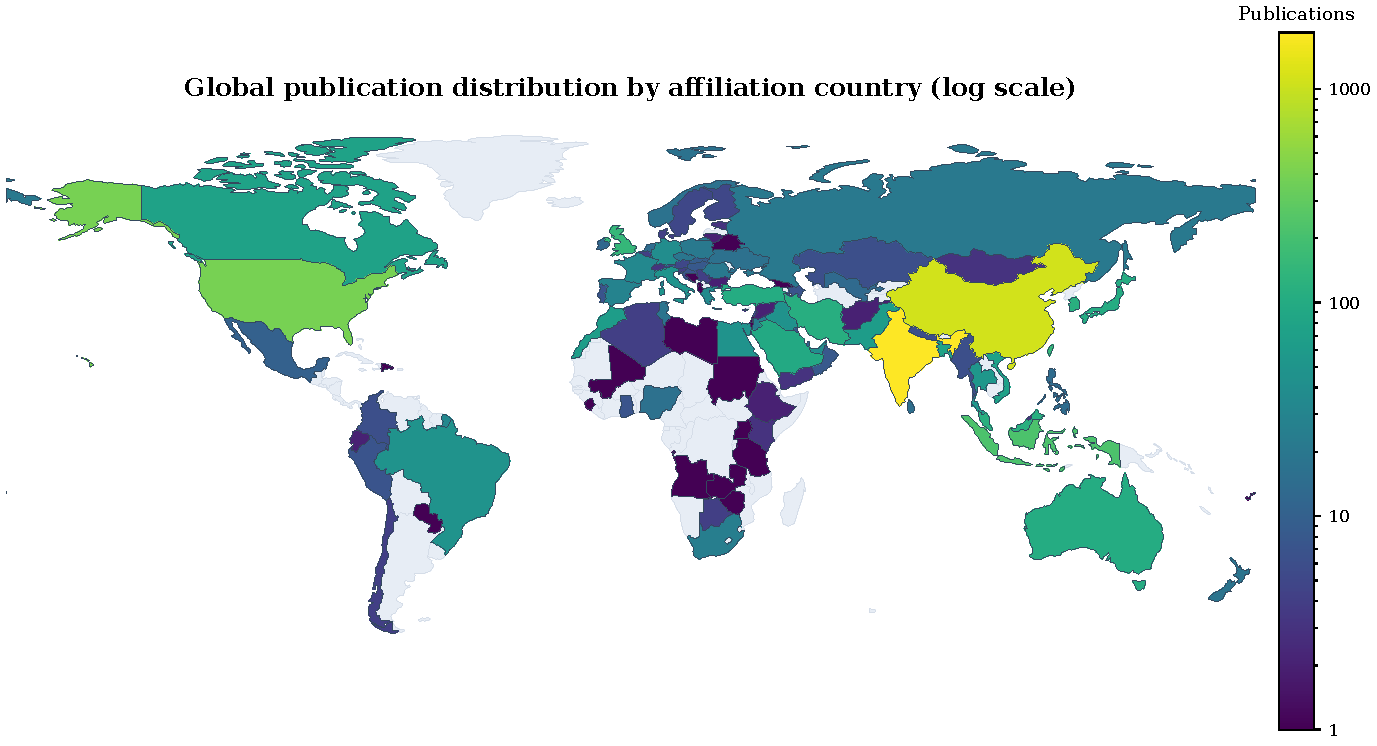
\includegraphics[width=\textwidth]
    {Fig_World_Publication_Map.pdf}
    \caption{Global distribution of computational stock-market forecasting
    publications by affiliation country. The map is based on \(4{,}971\)
    publications with geographically identifiable affiliation metadata from
    the cleaned \(4{,}974\)-publication bibliometric corpus. Country output
    was calculated using document-level full counting; therefore,
    internationally co-authored publications were assigned once to each
    participating country. Colour intensity is displayed on a logarithmic
    scale, while countries without identified contributions are shown in
    light grey. Three publications without usable affiliation information
    were excluded only from the geographical analysis.}
    \label{fig:world-publication-map}
\end{figure*}
\FloatBarrier

Figure~\ref{fig:world-publication-map} shows that publication activity is
geographically concentrated but globally distributed. India and China form
the two largest publication centres, followed by the United States. Strong
contributions are also visible across Southeast Asia, East Asia, Europe,
the Middle East, and Oceania. The geographical pattern demonstrates the
particularly strong role of Asian research communities in computational
stock-market forecasting, while also showing extensive participation from
North American, European, Middle Eastern, African, and Oceanian institutions.

The country counts represent publication participation rather than mutually
exclusive national ownership. A publication involving institutions from
several countries contributes to every participating country. Country
information was derived only from verified affiliation metadata and was not
inferred from author names, the stock market examined, the conference venue,
or the publisher's location.

To examine how the substantive orientation of the literature developed over
time, every publication in the cleaned corpus was assigned to one primary
application area using evidence from its title, abstract, author keywords,
and index keywords. A mutually exclusive primary classification was used so
that each publication contributed exactly once to the year-wise heatmap.
The resulting categories were price and index forecasting; direction, trend,
and regime prediction; return forecasting; volatility, risk, and uncertainty;
sentiment, news, and social-media analysis; trading, portfolio, and decision
support; high-frequency and market-microstructure forecasting; multi-asset
and cross-market forecasting; and general or multi-target applications.

\begin{figure*}[!t]
\centering
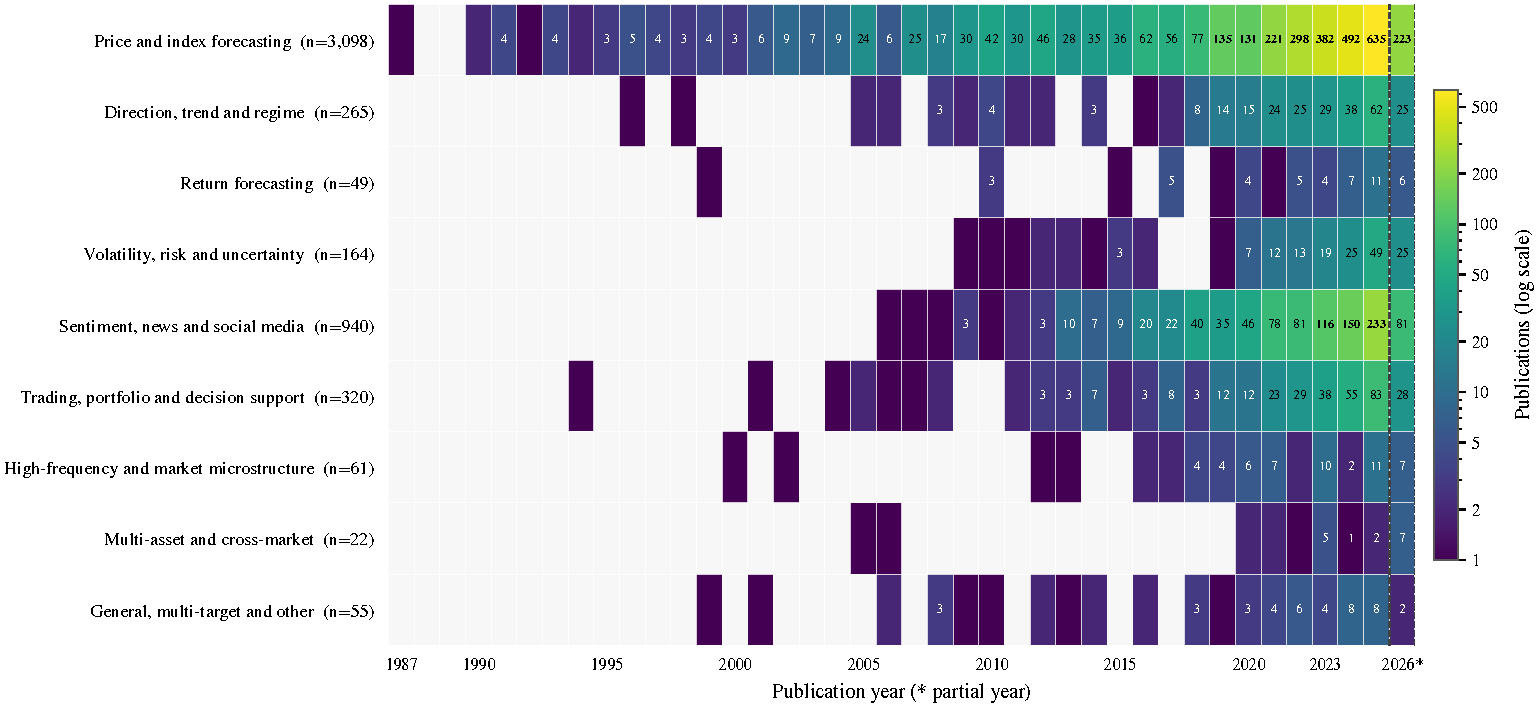
\includegraphics[
    width=\textwidth
]{Fig5_Application_Area_Annual_Heatmap_Q1.pdf}
\caption{Application-area publication trends in computational
stock-market forecasting from 1987 to 2026. Cell shading represents the
annual number of publications using a logarithmic colour scale, while
selected cell annotations report exact publication counts. Row labels
include the total number of publications assigned to each mutually
exclusive primary application area. The heatmap contains all 4,974
publications in the cleaned bibliometric corpus. The 2026 column,
identified by an asterisk and dashed boundaries, represents an
incomplete publication year and should not be interpreted as evidence
of a complete-year decline.}
\label{fig:application-area-trends}
\end{figure*}
\FloatBarrier

Figure~\ref{fig:application-area-trends} demonstrates that price and
index forecasting constituted the dominant application area throughout the
observed period. Its publication volume increased sharply after 2018 and
reached its highest complete-year level in 2025. This dominance indicates
that the principal orientation of the literature remained the prediction of
future stock or index values, even as the computational methods used for
that purpose became increasingly sophisticated.

Sentiment-, news-, and social-media-oriented forecasting formed the
second-largest application stream and expanded particularly rapidly after
2020. This growth reflects the increasing use of financial news, social
media, investor opinion, natural-language processing, pretrained language
models, and multimodal information in stock-market prediction.

Direction-, trend-, and regime-oriented studies also increased in recent
years, although their publication volume remained substantially lower than
that of price-level forecasting. Trading, portfolio, and decision-support
applications showed a visible but comparatively smaller expansion,
indicating growing interest in translating predictive outputs into
investment decisions and economic evaluation.

Volatility-, risk-, and uncertainty-oriented studies remained limited
during the earlier periods but became more visible after 2015. Likewise,
high-frequency and market-microstructure forecasting, multi-asset and
cross-market prediction, and explicitly return-oriented forecasting
remained specialized application areas. Their smaller publication counts
should not be interpreted as evidence of limited methodological importance;
rather, they indicate that these tasks constitute narrower and often more
data-intensive research streams.

The strong increase observed during 2021--2025 is consistent with the wider
growth of deep learning, transformer architectures, sentiment-aware models,
hybrid systems, graph-based learning, and multimodal forecasting. The
\(404\) publications indexed for 2026 represent partial-year coverage and
should therefore be interpreted separately from the complete annual counts.

At the institutional level, the most productive organizations are reported
in \supptableref{tab:top-institutions} after normalization of common affiliation-name
variants. Institution-level findings should be interpreted cautiously
because bibliographic databases may represent the same organization at the
university, campus, faculty, school, department, laboratory, or institutional
system level. Institutional names may also vary because of abbreviations,
translations, mergers, or changes in organizational structure. The
institutional results are therefore treated as indicators of research
concentration rather than as definitive organizational rankings.

\subsection{Citation impact of publication sources}

Citation-impact analysis was restricted to the 4,789
Scopus-indexed records retained in the cross-database deduplicated
corpus. This restriction ensured that publication-level citation
counts were derived from a single bibliographic database rather
than by combining database-specific citation measures. Source-title
variants were consolidated before aggregation, and sources were
ranked by total Scopus citations.

Table~\ref{tab:source-citation-impact} presents the ten leading
source titles. Expert Systems with Applications was the dominant
citation source, with 116 publications and 13,648 citations.
Applied Soft Computing ranked second after consolidation of its
source-title variants, with 40 publications and 3,292 citations.
Procedia Computer Science and IEEE Access followed with 3,057 and
2,732 citations, respectively. Neural Computing and Applications,
Neurocomputing, and Knowledge-Based Systems also constituted
important citation hubs within the field.

The ranking by aggregate citations differs from the ranking by
average citation impact. Knowledge-Based Systems recorded the
highest average among the listed sources, with 174.62 citations per
publication, followed by the IJCAI International Joint Conference
on Artificial Intelligence with 167.17 and Decision Support Systems
with 155.75. These high averages were based on comparatively small
numbers of publications and should therefore be interpreted
alongside publication volume.

The source-level citation structure confirms the close association
of computational stock-market forecasting with expert systems,
neural computation, soft computing, machine learning, and
decision-support research. Citation values should nevertheless be
interpreted cautiously because older publications have had more
time to accumulate citations, whereas recent transformer-based,
graph-based, and multimodal studies remain at an earlier stage of
citation development.

\begin{table*}[!t]
\centering
\caption{Top 10 source titles by aggregate Scopus citation count
within the Scopus-indexed component of the deduplicated review
corpus. Citation counts reflect the Scopus metadata snapshot
finalized on 19 June 2026.}
\label{tab:source-citation-impact}

\tiny
\setlength{\tabcolsep}{3.6pt}
\renewcommand{\arraystretch}{1.05}

\begin{tabular}{@{}rlrrr@{}}
\toprule
Rank &
Source title &
Publications &
Total citations &
Average citations \\
\midrule

1 &
Expert Systems with Applications &
116 &
13,648 &
117.66 \\

2 &
Applied Soft Computing &
40 &
3,292 &
82.30 \\

3 &
Procedia Computer Science &
45 &
3,057 &
67.93 \\

4 &
IEEE Access &
66 &
2,732 &
41.39 \\

5 &
Neural Computing and Applications &
38 &
2,647 &
69.66 \\

6 &
Neurocomputing &
19 &
2,601 &
136.89 \\

7 &
Knowledge-Based Systems &
13 &
2,270 &
174.62 \\

8 &
Decision Support Systems &
8 &
1,246 &
155.75 \\

9 &
Information Sciences &
16 &
1,103 &
68.94 \\

10 &
        International Joint Conference on Artificial Intelligence &
6 &
1,003 &
167.17 \\

\bottomrule
\end{tabular}

\vspace{3pt}
\begin{minipage}{0.97\textwidth}
\footnotesize
\textit{Note:} The ranking was calculated from the 4,789
Scopus-indexed records retained in the cross-database deduplicated
corpus. Source-title variants were consolidated before aggregation.
Web of Science and IEEE Xplore citation values were not combined
with Scopus citation counts. Average citations were calculated as
total Scopus citations divided by the number of retained
Scopus-indexed publications for each normalized source title.
\end{minipage}
\end{table*}
\FloatBarrier   



\subsection{Highly cited documents and intellectual foundations}

The highly cited documents reveal the intellectual foundations of stock price prediction research. Early influential studies were dominated by support vector machines, hybrid statistical--machine-learning models, and artificial neural networks. These works established the feasibility of applying computational intelligence to noisy, nonlinear, and non-stationary financial time series.

Later highly cited studies introduced event-driven prediction, deep learning architectures, financial-news-based textual analysis, CNN--RNN--LSTM variants, and attention-based models. This citation trajectory indicates a clear methodological progression. The field initially relied on classical machine learning and hybrid statistical models, then moved toward neural networks and deep learning, and more recently expanded into news-driven, sentiment-aware, attention-based, and hybrid architectures.

Therefore, the highly cited documents do not merely represent individual influential papers. They also mark the major methodological transitions that shaped stock price prediction research over the last four decades. This citation-based evidence provides the foundation for the later thematic and systematic technical review sections, where each method family is examined in greater detail.


\section{Science Mapping and Thematic Structure}
\label{sec:science-mapping}

The analyses in this section use different evidence bases according
to their metadata requirements. Author co-authorship, country
collaboration, and keyword co-occurrence analyses were conducted using
the deduplicated bibliometric corpus of 5,022 records.
Cited-reference co-citation and document-level bibliographic-coupling
analyses were conducted using an independently deduplicated,
reference-preserving Scopus dataset of 4,792 records.

The thematic map and thematic-evolution analyses used the
4,610-record complete-year corpus covering 1987--2025, of which
4,528 records contained at least one usable normalized keyword.
The 485-study high-priority subset was reserved for the systematic
technical synthesis and methodological audit reported from
Section~\ref{sec:problem-formulation} onward. The evidence base and
denominator used for each analysis are stated in the corresponding
table and figure caption.

Table~\ref{tab:mapping-settings} summarizes the evidence
bases, counting methods, selection thresholds, and analytical
settings used for the science-mapping and thematic analyses.
\begin{table*}[!t]
\centering
\caption{Science-mapping and thematic-analysis settings.}
\label{tab:mapping-settings}

\scriptsize
\setlength{\tabcolsep}{3pt}
\renewcommand{\arraystretch}{1.15}

\begin{tabular}{@{}p{2.8cm}p{2.8cm}p{9.0cm}@{}}
\toprule
Analysis
& Evidence base
& Final settings \\
\midrule

Author co-authorship
& 5,022-record bibliometric corpus
& Fractional counting; bibliographic author-name entities as the
unit of analysis; minimum of 5 documents and 49 citations per
entity; maximum of 25 authors per document; 275 retained
author-name entities; 19 clusters; 1,164 links; total link strength
of 866.00. \\

Country collaboration
& 5,022-record bibliometric corpus
& Fractional counting; countries as the unit of analysis; minimum
of 10 documents per country; 48 retained countries; 6 clusters;
322 collaboration links; total link strength of 731.00. \\

Cited-reference co-citation
& 4,792 independently deduplicated Scopus records
& Cited references as the unit of analysis; fractional counting;
minimum of 20 citations per cited reference; 38 verified thesaurus
replacement mappings; 150 retained cited references; one connected
component; 5 clusters; 5,230 links; total link strength of
2,907.19. \\

Document bibliographic coupling
& 4,792 independently deduplicated Scopus records
& Documents as the unit of analysis; fractional counting; minimum
of 10 citations per document; 1,319 threshold-eligible documents;
the 300 documents with the greatest total link strength were
retained; one connected component; 10 clusters; 19,828 links;
total link strength of 4,863.43. \\

Keyword co-occurrence
& 5,022-record bibliometric corpus
& Author keywords; full counting; thesaurus-assisted normalization
using 200 direct rules (114 replacements and 86 exclusions);
minimum occurrence threshold of 9; 175 threshold-eligible keywords
retained; 11 clusters; 3,257 links; total link strength of 12,325. \\

Thematic map
& 4,610 complete-year records covering 1987--2025
& Of the 4,610 records, 4,528 retained at least one usable normalized
keyword; 250 normalized source keywords; minimum frequency of 5;
Louvain clustering; random seed 1234; stemming disabled; five
thematic communities. \\

Thematic evolution
& 4,610 complete-year records covering 1987--2025
& Six publication periods: 1987--2005, 2006--2015, 2016--2020,
2021--2022, 2023--2024, and 2025; 27 thematic nodes and
69 inter-period links. \\

\bottomrule
\end{tabular}

\vspace{2pt}
\begin{minipage}{\textwidth}
\footnotesize
\textit{Note:} VOSviewer version 1.6.21 was used for the network
analyses. For keyword co-occurrence, a minimum occurrence threshold
of nine yielded 175 retained author keywords after application of
200 direct thesaurus rules, comprising 114 replacement rules and
86 exclusion rules.
\end{minipage}
\end{table*}
\FloatBarrier


\subsection{Co-authorship network} 
Author-level collaboration was examined using a co-authorship network generated from the deduplicated bibliometric corpus. Fractional counting was applied to reduce the disproportionate influence of publications involving large author teams. Bibliographic author-name entities were required to have at least five publications and 49 citations to be retained, while documents containing more than 25 authors were excluded from the analysis. The selected thresholds retained the principal collaboration groups while preserving the readability of the network.

The final network contained 275 bibliographic author-name entities distributed across 19 collaboration clusters. It included 1,164 co-authorship links and had a total link strength of 866.00. All 275 retained entities belonged to a single connected component, and no isolated entities were present. The complete network-construction settings are reported in \supptableref{tab:author-coauthorship-settings}. \suppfigref{fig:author-coauthorship-network} shows that the collaboration structure is globally connected
but highly modular. Node size represents publication output, link thickness denotes fractional co-authorship strength, and colours identify collaboration clusters generated by VOSviewer.


A dense group of interconnected clusters is visible around author-name entities such as Wang Y., Li Y., Chen Y., Zhang Y., Wang J., Li X., and Liu Y. Another visually distinct collaboration region contains entities such as Singh S., Kumar S., Singh A., Sharma A., Gupta A., Patel M., Nayak S.C., and Das S. Several smaller compact groups also occur near the periphery of the network.

Although some collaboration groups appear spatially separated in the visualization, the connected-component analysis confirms that they remain linked through direct or indirect co-authorship paths. The large visual distances therefore indicate comparatively weak bridging relationships rather than completely disconnected research communities. The presence of 19 clusters within one connected component suggests that stock price prediction research contains several specialized collaboration communities embedded within a broader author network.

These findings should be interpreted cautiously because abbreviated author names and common surnames may merge publications belonging to different researchers or separate records associated with the same individual. Accordingly, the mapped nodes are treated as bibliographic author-name entities rather than fully disambiguated individual researchers. Geographical or institutional identities should not be inferred solely from author names without verifying affiliation metadata.


\subsection{Country collaboration network}

Country-level scientific collaboration was examined using a co-authorship network constructed from the affiliation metadata of the deduplicated bibliometric corpus. Fractional counting was used so that publications involving several participating countries did not exert a disproportionate influence on the collaboration structure. Countries were required to have at least 10 associated documents to be retained in the final network.

The resulting network contained 48 countries organized into 6 collaboration clusters, with 322 links and a total link strength of 731.00. In the network visualization, node size represents the number of publications associated with a country, whereas link thickness represents fractional bilateral collaboration strength. Countries positioned closer together generally exhibit stronger or more frequent collaboration relationships.

Figure~\ref{fig:country-collaboration-network} presents the resulting country-level collaboration network. India and China form the two largest publication hubs. India show extensive collaboration with countries from Asia, the Middle East, Europe, and Africa, including Saudi Arabia, Iraq, Malaysia, the United Kingdom, and South Africa. China is connected with the United States, Bangladesh, Japan, Indonesia, Hong Kong, Macao, Australia, and several European research communities.

The United States and the United Kingdom occupy comparatively central positions in the visual topology of the network and connect several regional collaboration groups. Australia, Malaysia, South Korea, Iran, Canada, Singapore, Saudi Arabia, Indonesia, Germany, and France also function as visible secondary hubs. Overall, the network indicates that stock price prediction research is concentrated strongly in Asia but is supported by extensive cross-regional collaboration involving North American, European, Middle Eastern, African, and Oceanian institutions.

The six collaboration clusters should not be interpreted as completely independent national research communities. Considerable overlap exists among the clusters, indicating that the field has developed through multiple interconnected regional and international partnerships rather than through isolated country-level research systems.

\begin{figure*}[htbp]
    \centering
    \includegraphics[
        width=\textwidth,
        trim=10 10 10 10,
        clip
    ]{Fig_Country_Collaboration_Network_Final.pdf}
    \caption{Country-level co-authorship network in stock price prediction research. The network contains 48 countries distributed across 6 collaboration clusters, with 322 links and a total link strength of 731.00. Node size represents country-level publication output, link thickness denotes fractional collaboration strength, and colours identify collaboration clusters generated by VOSviewer. The network highlights the major contributions of India and China, the comparatively central positions of the United States and the United Kingdom, and extensive cross-regional collaboration among Asian, European, North American, Middle Eastern, African, and Oceanian research communities.}
    \label{fig:country-collaboration-network}
\end{figure*}
\FloatBarrier



\suppfigref{fig:country-collaboration-overlay}, presents the temporal
overlay visualization of the country-level collaboration network. Node colour represents the average publication year of the records associated with each country. Although the database searches covered 1985--2026, the retrieved
bibliometric corpus contained publications from 1987--2026. The
displayed average-publication-year scale ranges from 2019 to 2023
because the average years of the retained country nodes are
concentrated within this interval. The overlay should therefore be interpreted comparatively: countries closer to the earlier end of the scale have relatively earlier average research activity, whereas countries closer to the later end show comparatively more recent publication activity.

\subsection{Cited-reference co-citation analysis}
\label{subsec:cocitation_analysis}

Cited-reference co-citation analysis was conducted to identify the
intellectual foundations that have jointly shaped computational stock-price
prediction research. Unlike direct-citation analysis, which traces explicit
citation flows between publications, co-citation analysis measures how
frequently two references are cited together by later documents. References
that are repeatedly co-cited are therefore interpreted as belonging to a
shared intellectual or methodological knowledge base.

The analysis was performed using the native Scopus export because the
available IEEE Xplore records contained reference counts rather than complete
cited-reference lists, while the Web of Science export did not provide
sufficiently populated cited-reference metadata for an equivalent network.
The original Scopus export contained 4,832 records, of which 4,802 contained
non-empty cited-reference information before deduplication. Independent
within-source deduplication based on DOI and normalized title information
retained 4,792 records. Among these, 4,762 records contained cited references,
corresponding to a reference-coverage rate of 99.37\%.

The independently deduplicated Scopus co-citation dataset contained three
more records than the 4,789 Scopus records retained in the principal
cross-database deduplication workflow. This difference resulted from the use
of a separate reference-preserving, within-source duplicate-resolution
procedure and does not modify the PRISMA record counts reported for the main
bibliometric corpus.

The network was constructed in VOSviewer version 1.6.21 using cited
references as the unit of analysis and fractional counting as the counting
method. Fractional counting was selected to reduce the disproportionate
influence of citing documents containing exceptionally long reference lists.
A minimum threshold of 20 citations per cited reference was applied.
Bibliographic variants caused by abbreviated journal names, incomplete author
attribution, punctuation differences, omitted issue information, and
alternative source-title formats were manually adjudicated. A final
cited-reference thesaurus containing 38 verified replacement mappings was
then applied before regeneration of the definitive network.

After normalization and thresholding, 150 cited references were retained.
All references belonged to a single connected component, and no isolated
references remained. The network comprised five clusters, 5,230
co-citation links, and an aggregate link strength of 2,907.19. The complete
connectivity of the network indicates that the major methodological and
theoretical foundations of stock-price prediction are not isolated research
traditions but form an interconnected intellectual structure.

The most prominent intellectual foundations include the original
long short-term memory formulation, general deep-learning foundations,
tree-boosting methods, adaptive gradient-based optimization, attention and
transformer architectures, bidirectional language representation learning,
sentiment-based market prediction, and applied LSTM-based financial-market
forecasting. Their simultaneous presence in the network demonstrates that
the field has developed through the convergence of neural sequence modelling,
classical and ensemble machine learning, optimization techniques,
natural-language processing, and domain-specific financial forecasting.
The five detected clusters therefore represent related but distinguishable
knowledge bases rather than completely independent methodological schools.

Figure~\ref{fig:cited_reference_cocitation} presents the final
cited-reference co-citation network. Node size represents the citation weight
of each reference, link thickness represents the strength of co-citation
relationships, and node colour denotes cluster membership. The spatial
proximity of references reflects their relatedness based on normalized
co-citation strength.

\begin{figure*}[!htbp]
    \centering
    \includegraphics[
        width=0.98\textwidth
    ]{Fig_Cited_Reference_Cocitation_Network_Final.pdf}
    \caption{
        Cited-reference co-citation network of computational
        stock-price prediction research. The network was generated using
        fractional counting and a minimum threshold of 20 citations per
        cited reference. Node size represents citation weight, link thickness
        represents co-citation strength, and node colour indicates membership
        in one of the five detected intellectual clusters. The final network
        contains 150 cited references, 5,230 links, and a total link strength
        of 2,907.19.
    }
    \label{fig:cited_reference_cocitation}
\end{figure*}
\FloatBarrier

Table~\ref{tab:cocitation_network_summary} summarizes the final
settings and structural characteristics of the cited-reference
co-citation network. The network comprised 150 cited references
organized into five clusters within a single connected component,
with 5,230 links and a total link strength of 2,907.19.

\begin{table}[!htbp]
\centering
\caption{
    Final settings and structural characteristics of the
    cited-reference co-citation network.
}
\label{tab:cocitation_network_summary}
\begin{tabular}{lr}
\hline
\textbf{Network characteristic} & \textbf{Value} \\
\hline
Raw Scopus records & 4,832 \\
Independently deduplicated Scopus records & 4,792 \\
Records containing cited references & 4,762 \\
Cited-reference coverage & 99.37\% \\
Minimum citations per cited reference & 20 \\
Thesaurus replacement mappings & 38 \\
Selected cited references & 150 \\
Connected components & 1 \\
Largest connected component & 150 \\
Isolated references & 0 \\
Clusters & 5 \\
Links & 5,230 \\
Total link strength & 2,907.19 \\
Counting method & Fractional \\
VOSviewer version & 1.6.21 \\
\hline
\end{tabular}
\end{table}
\FloatBarrier
% \subsection{Bibliographic coupling analysis}
% \subsection{Document-level bibliographic coupling}
\label{subsec:bibliographic_coupling}
\subsection{Document-level bibliographic-coupling analysis}
\label{subsec:document-bibliographic-coupling}
Document-level bibliographic coupling was used to identify the active
research fronts within computational stock-price prediction. Two documents
are bibliographically coupled when they cite one or more references in
common. Whereas cited-reference co-citation analysis reveals the historical
and intellectual foundations of a field, bibliographic coupling emphasizes
the relationships among the citing documents themselves and is therefore
particularly suitable for identifying contemporary methodological
communities.

The analysis was conducted using the independently deduplicated native
Scopus dataset containing 4,792 records. A minimum threshold of 10 citations
per document was applied, which was satisfied by 1,319 publications. To
retain the most structurally relevant publications while preserving visual
interpretability, the 300 documents with the greatest total bibliographic
coupling link strength were selected. These documents represented 22.74\%
of the threshold-eligible publications. Selection was performed
algorithmically using total link strength; documents were not manually
included or excluded on the basis of their titles, authors, journals, or
reported findings.

The network was generated in VOSviewer version 1.6.21 using documents as
the unit of analysis and fractional counting as the counting method.
Fractional counting was used to reduce the disproportionate contribution of
documents containing unusually extensive reference lists. The resulting
network contained 300 documents, all of which belonged to a single connected
component. No isolated documents were present. The network comprised 10
clusters, 19,828 bibliographic-coupling links, and a total link strength of
4,863.

Table~\ref{tab:bibliographic_coupling_clusters} summarizes the ten
bibliographic-coupling clusters, including their document counts,
relative shares, mean publication years, and principal research
themes.

\begin{table*}[!htbp]
\centering
\caption{Document-level bibliographic-coupling clusters and their
principal research themes.}
\label{tab:bibliographic_coupling_clusters}
\begin{tabular}{c r r r p{6.0cm}}
\hline
\textbf{Cluster} &
\textbf{Documents} &
\textbf{Share (\%)} &
\textbf{Mean year} &
\textbf{Interpretive theme} \\
\hline
1 & 91 & 30.33 & 2023.03 &
Recent deep-learning, hybrid-model, and optimization reviews \\
2 & 78 & 26.00 & 2015.26 &
Foundational artificial intelligence, artificial neural networks,
and computational-intelligence research \\
3 & 64 & 21.33 & 2021.08 &
Sentiment, news, text mining, and intelligent trading systems \\
4 & 48 & 16.00 & 2020.56 &
Machine-learning techniques, data design, and market-efficiency
assessment \\
5 & 7 & 2.33 & 2010.86 &
Morphological neural and evolutionary forecasting \\
6 & 4 & 1.33 & 2020.50 &
Mode-decomposition and extreme-learning-machine hybrids \\
7 & 2 & 0.67 & 2021.50 &
Machine-learning-assisted portfolio optimization \\
8 & 2 & 0.67 & 2008.00 &
Factor-model versus neural-network forecasting \\
9 & 2 & 0.67 & 2003.50 &
Genetic--neural mixture and hybrid architectures \\
10 & 2 & 0.67 & 2023.00 &
Functional-link neural networks with heuristic optimization \\
\hline
\end{tabular}
\end{table*}
\FloatBarrier

The cluster-size distribution was strongly asymmetric. The four largest
clusters contained 281 documents, representing 93.67\% of the selected
network, whereas the remaining six clusters contained only 19 documents.
Accordingly, the first four clusters were interpreted as the dominant
research fronts, while the smaller clusters were treated as specialized
methodological niches rather than research streams of equivalent scope.

Cluster~1 was the largest community, containing 91 documents
(30.33\%), and represented recent reviews and applications of deep
learning, hybrid neural architectures, genetic algorithms, and related
optimization methods. Its mean publication year of 2023.03 indicates that
this cluster captures the recent consolidation of deep-learning-based stock
forecasting.

Cluster~2 contained 78 documents (26.00\%) and represented the broader
artificial-intelligence and computational-intelligence foundation of the
field. Its leading studies included surveys of artificial neural networks,
soft computing, computational intelligence, and critical assessments of
artificial intelligence in financial-market forecasting.

Cluster~3 contained 64 documents (21.33\%) and was centred on
information-rich forecasting using investor sentiment, financial news,
text mining, social-media information, fundamental analysis, technical
analysis, and intelligent trading systems. This cluster reflects the
transition from exclusively numerical price histories towards heterogeneous
and unstructured information sources.

Cluster~4 contained 48 documents (16.00\%) and focused on practical
machine-learning forecasting, data and feature design, scientometric
assessment, directional prediction, and the relationship between predictive
modelling and market efficiency. The cluster therefore connects algorithmic
performance with broader questions concerning data quality, empirical
validation, and the economic interpretation of predictive results.

The remaining clusters represented specialized methodological niches.
Cluster~5 captured morphological neural and evolutionary forecasting;
Cluster~6 combined mode-decomposition procedures with extreme learning
machines; Cluster~7 connected machine-learning prediction with portfolio
optimization; Cluster~8 compared conventional financial factor models with
artificial neural networks; Cluster~9 represented early genetic--neural
mixture and hybrid architectures; and Cluster~10 focused on functional-link
artificial neural networks optimized through Rao and set-algebra-based
heuristics.

Overall, the bibliographic-coupling structure show that contemporary
stock-price prediction research is dominated by four interconnected
directions: deep and hybrid learning, general artificial and computational
intelligence, sentiment- and text-enhanced forecasting, and practical
machine-learning design and evaluation. The smaller clusters preserve
specialized algorithmic traditions but occupy peripheral positions relative
to these dominant research fronts.


\subsection{Keyword co-occurrence analysis}

Keyword co-occurrence analysis was conducted to identify the conceptual structure of stock price prediction research. The analysis was performed using VOSviewer on the deduplicated bibliometric corpus. Keywords were mapped using full counting, and node size was interpreted as keyword occurrence frequency, while link strength represented the intensity of co-occurrence between keyword pairs.

Figure~\ref{fig:keyword-cooccurrence-network} presents the keyword co-occurrence network. The map show that the field is organized around several major conceptual centres. The most prominent terms include \textit{financial markets}, \textit{forecasting}, \textit{stock price prediction}, \textit{stock market prediction}, \textit{long short-term memory}, \textit{deep learning}, \textit{machine learning}, \textit{LSTM}, \textit{sentiment analysis}, \textit{time series}, \textit{prediction models}, and \textit{neural networks}. These keywords indicate that stock price prediction research has evolved into a computational-intelligence-driven forecasting domain, combining financial time-series modelling, machine learning, deep learning, natural language processing, and optimization-based approaches.



The VOSviewer clusters reveal distinct but interconnected research themes. One cluster is centred on classical forecasting and neural-network-based time-series prediction, including terms such as \textit{forecasting}, \textit{time series}, \textit{neural networks}, \textit{stock price forecasting}, and \textit{artificial intelligence}. A second cluster is associated with financial-market prediction, deep learning, sentiment analysis, data mining, and decision-making. A third cluster emphasizes sequence-modelling approaches, including \textit{LSTM}, \textit{prediction models}, \textit{short term memory}, \textit{ARIMA}, and \textit{CNN}. Another important cluster contains \textit{stock price prediction}, \textit{long short-term memory}, \textit{convolutional neural networks}, and \textit{deep neural networks}, reflecting the dominance of deep learning architectures in recent stock forecasting studies.

Keyword co-occurrence analysis was conducted using author keywords
from the 5,022-record deduplicated bibliometric corpus. Full counting
was applied in VOSviewer version 1.6.21. A validated thesaurus
containing 200 direct normalization rules was used, comprising
114 replacement rules for spelling variants, abbreviations,
singular--plural forms, and synonymous expressions, and 86 exclusion
rules for generic, corpus-defining, malformed, or non-discriminating
terms. A minimum occurrence threshold of nine was applied. All
175 keywords meeting the threshold were retained, producing a network
of 11 clusters, 3,257 links, and a total link strength of 12,325.

The keyword network also highlights specialized subfields such as attention mechanisms, optimization, fuzzy systems, support vector regression, random forests, decision trees, reinforcement learning, technical indicators, and sentiment-driven forecasting. Overall, the keyword co-occurrence structure confirms that stock price prediction has moved beyond single-model time-series forecasting and now involves hybrid computational intelligence, deep neural architectures, textual sentiment signals, and optimization-based modelling.
\begin{figure*}[htbp]
    \centering
    \includegraphics[width=\textwidth]{Fig_Keyword_Cooccurrence_Network.pdf}
    \caption{Normalized author-keyword co-occurrence network of
computational stock-market forecasting research based on the
5,022-record deduplicated bibliometric corpus. The network contains
175 threshold-eligible keywords organized into 11 clusters, with
3,257 links and a total link strength of 12,325. Keyword variants,
abbreviations, spelling differences, and synonymous expressions were
consolidated using a validated thesaurus containing 114 replacement
rules, while 86 generic or non-discriminating terms were excluded.
Node size represents keyword occurrence frequency, link thickness
denotes co-occurrence strength, and node colour indicates cluster
membership.}
    \label{fig:keyword-cooccurrence-network}
\end{figure*}
\FloatBarrier

\subsection{Thematic map of the conceptual structure}
\label{subsec:thematic_map}

A thematic map was constructed to examine the conceptual structure of
computational stock-price prediction research. The initial merged corpus
contained 5,022 records, of which 5,014 had valid publication-year
information. Because 2026 represented an incomplete publication year at the
time of analysis, 404 records published in 2026 were excluded from the
primary thematic analysis. The resulting complete-year corpus contained
4,610 records covering the period from 1987 to 2025.

The keyword-field audit revealed that the author-keyword and index-keyword
columns in the prepared merged dataset were exact duplicates. The two fields
were therefore not concatenated or analysed as independent sources.
Instead, one copy was retained and transformed into a normalized
source-keyword field. Spelling variants, abbreviations, plural forms, and
methodological synonyms were mapped to canonical terms, while
corpus-defining and non-discriminating expressions were removed.
After normalization, 4,528 publications retained at least one usable
keyword.

The thematic map was generated using 250 normalized source keywords with a
minimum frequency of five. Louvain community detection was employed with a
fixed random seed of 1234, and stemming was disabled to preserve the
interpretability of technical expressions. The horizontal axis represents
the relevance degree or centrality of a theme, while the vertical axis
represents its development degree or density. Bubble size reflects the
frequency of the terms belonging to each thematic cluster.

Five thematic communities were identified, as summarized in
Table~\ref{tab:thematic_map_clusters}. Artificial neural networks and
artificial intelligence occupied the motor-theme quadrant. This cluster
combined high centrality with the highest density and therefore represented
a well-developed research stream that was also strongly integrated with the
wider conceptual structure of the field.

The long short-term memory and deep-learning cluster was located close to
the boundary between the basic- and motor-theme quadrants. It exhibited the
highest centrality in the map, indicating strong relationships with other
research streams. Its position close to the median density boundary suggests
that it functions as a broad foundational theme while simultaneously moving
towards the status of a highly developed motor theme.

Machine learning and support vector machines were positioned near the
centrality boundary in the basic-theme region. This cluster represented a
fundamental and widely connected methodological foundation, although its
internal development degree was lower than that of the motor and niche
themes.

Sentiment analysis and data mining occupied the niche-theme quadrant. The
cluster was internally developed but less strongly connected to the central
methodological structure. It represented a specialized information-driven
stream involving social media, natural-language processing, financial news,
and related textual information.

Risk management and trading strategies appeared in the
emerging-or-declining quadrant. Evidence from the thematic-evolution
analysis showed that this stream became particularly visible in the most
recent period. It was therefore interpreted as an emerging theme rather
than as a declining research direction.


\begin{table*}[!htbp]
\centering
\caption{Final thematic-map clusters and their conceptual positions.}
\label{tab:thematic_map_clusters}
\begin{tabular}{c r r r p{5.2cm} p{3.3cm}}
\hline
\textbf{Cluster} &
\textbf{Terms} &
\textbf{Centrality} &
\textbf{Density} &
\textbf{Principal theme} &
\textbf{Interpretation} \\
\hline
1 & 74 & 1.3145 & 3.7039 &
Long short-term memory and deep learning &
Basic--motor boundary \\
2 & 47 & 0.9794 & 3.5546 &
Machine learning and support vector machines &
Basic-theme boundary \\
3 & 77 & 1.0891 & 4.2361 &
Artificial neural networks and artificial intelligence &
Motor theme \\
4 & 36 & 0.7005 & 3.7304 &
Sentiment analysis and data mining &
Niche theme \\
5 & 16 & 0.4082 & 3.3469 &
Risk management and trading strategies &
Emerging theme \\
\hline
\end{tabular}
\end{table*}
\FloatBarrier

Figure~\ref{fig:thematic-map} presents the final thematic map. The absence of
themes located unambiguously deep within every quadrant should not be
interpreted as a methodological deficiency. Instead, the positions reflect
the empirical centrality and density structure of the normalized keyword
network.
\begin{figure*}[t]
\centering
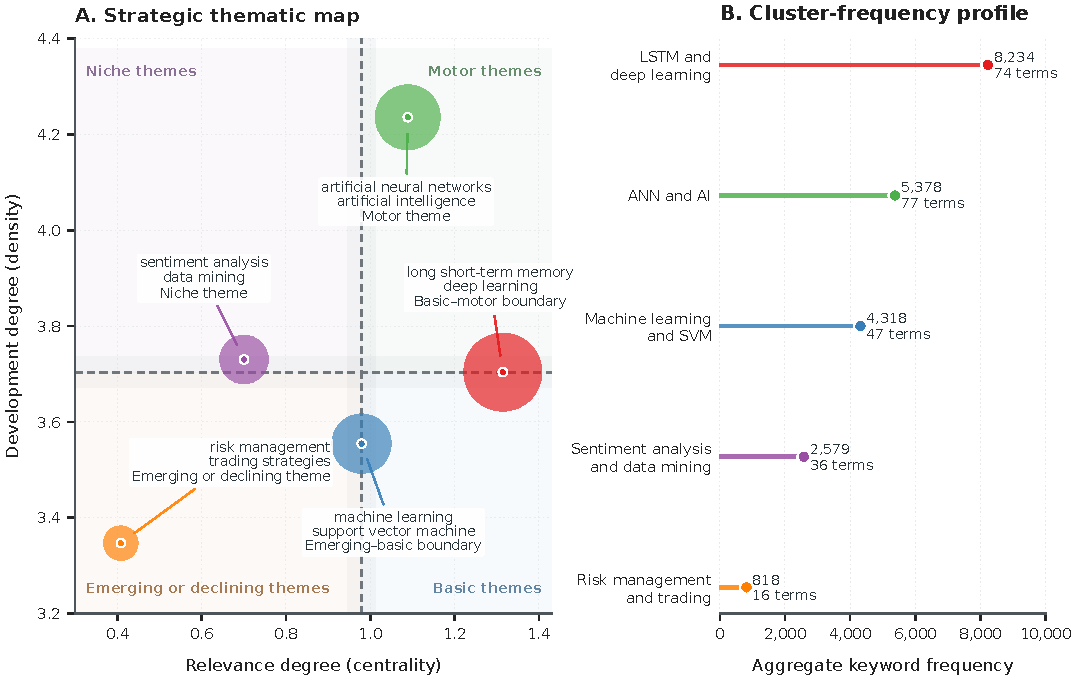
\includegraphics[
  width=\textwidth
]{Figure9_Thematic_Map_SCIE_Q1_Final.pdf}
\caption{Strategic thematic structure of normalized source-keyword
clusters in computational stock price prediction research. Panel~A
positions the five thematic communities according to normalized
centrality and density, while bubble area is proportional to aggregate
cluster keyword frequency. Dashed lines indicate the median centrality
(\(C_{\mathrm{median}}=0.9794\)) and density
(\(D_{\mathrm{median}}=3.7039\)) thresholds, and the lightly shaded
bands identify clusters located close to those thresholds. Panel~B
reports aggregate keyword frequency and the number of retained
normalized terms in each cluster. Artificial neural networks and
artificial intelligence constitute a motor theme, whereas sentiment
analysis and data mining form a niche theme. Risk management and
trading strategies occupy the emerging-or-declining quadrant. Long
short-term memory and deep learning lie on the basic--motor boundary,
while machine learning and support vector machines lie on the
emerging--basic boundary.}
\label{fig:thematic-map}
\end{figure*}
\FloatBarrier
\subsection{Thematic evolution}
\label{subsec:thematic_evolution}

Thematic-evolution analysis was conducted to examine how the principal
conceptual streams changed across successive stages of the field's
development. Six periods were used to preserve the historical progression
of computational stock-price prediction while accounting for the rapid
increase in publication activity after 2020. The periods were
1987--2005, 2006--2015, 2016--2020, 2021--2022, 2023--2024, and 2025. Their corresponding publication counts are reported in the \supptableref{tab:thematic_evolution_periods}.

The first period, 1987--2005, contained 107 publications and was
characterized by artificial neural networks, backpropagation, time-series
analysis, genetic algorithms, and data mining. These themes represent the
early computational foundations of the field.

During 2006--2015, artificial neural networks remained prominent, while
genetic algorithms, support vector machines, fuzzy logic, and data mining
developed into distinguishable methodological streams. This period marked
the expansion of conventional machine learning and computational
intelligence beyond the earlier neural-network-centred structure.

The 2016--2020 period represented a major transition. Machine learning and
long short-term memory emerged as central themes, while artificial neural
networks continued to provide an established conceptual foundation.
Technical indicators also appeared as a distinct input-oriented stream.
The period therefore reflects the movement from traditional computational
intelligence towards deep sequence learning and broader machine-learning
frameworks.

During 2021--2022, machine learning and long short-term memory became the
dominant persistent themes. Artificial neural networks continued to connect
with these newer architectures, while sentiment analysis developed into a
recognizable information-driven research stream.

In 2023--2024, long short-term memory and machine learning retained their
structural importance. Sentiment analysis became more consolidated, while
autoregressive integrated moving average modelling, decentralized finance,
and technical indicators formed additional specialized paths. These
developments show that contemporary research combines deep learning with
statistical modelling, alternative financial environments, and
information-rich predictors.

The 2025 period retained machine learning, long short-term memory, and
sentiment analysis as major themes. Risk management became a prominent
emerging stream, reflecting growing attention to decision consequences,
portfolio exposure, trading strategies, and financially meaningful
evaluation rather than predictive accuracy alone.

Three particularly persistent trajectories were observed. Artificial neural
networks extended from the earliest period through the development of modern
machine-learning and deep-learning research. Long short-term memory formed a
continuous trajectory from 2016--2020 through 2025. Machine learning
similarly remained continuous from 2016 onward, while sentiment analysis
showed sustained continuity from 2021--2022 to 2025.

The final thematic-evolution network contained 27 thematic nodes and 69
inter-period links. The connecting flows represent shared keyword content
and conceptual continuity between themes in adjacent periods. They should
not be interpreted as causal relationships, exact dates of methodological
invention, or proof that a method first appeared during a particular period.

Figure~\ref{fig:thematic-evolution-sankey} presents the final thematic-evolution
diagram.


\begin{figure*}[t]
\centering
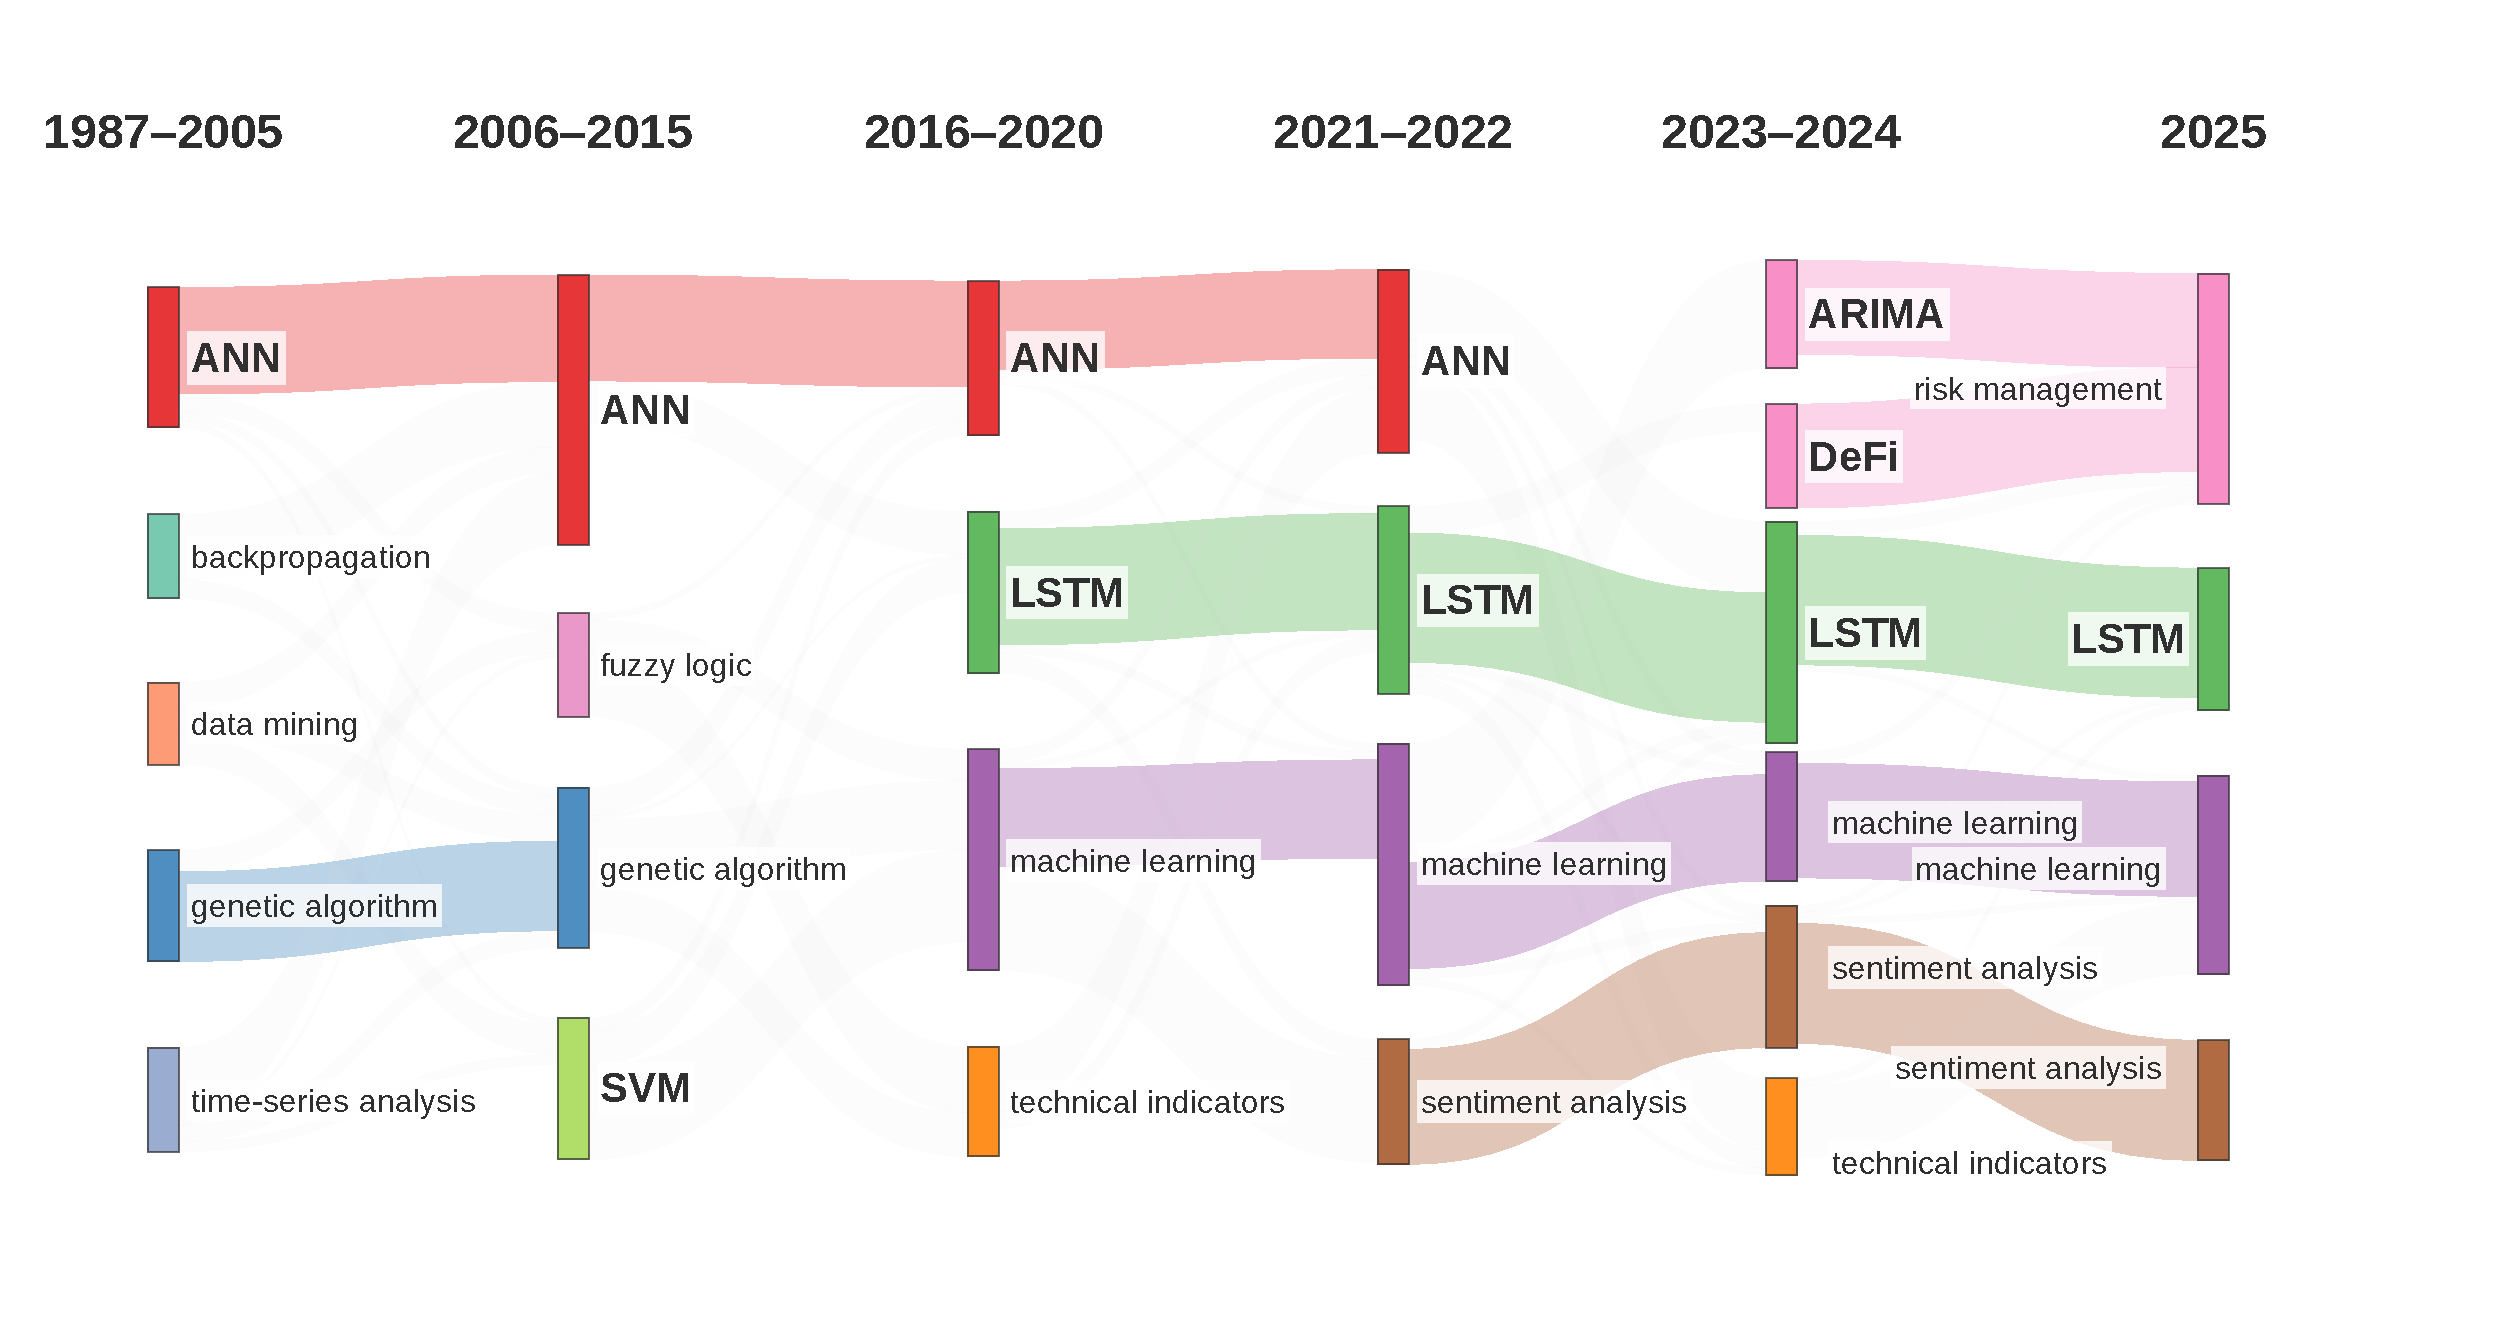
\includegraphics[
  width=\textwidth,
  trim=0 0 0 0,
  clip
]{Thematic_Evolution_Sankey_SCIE_Q1_Final.pdf}
\caption{Thematic evolution of computational stock-market forecasting
across six publication periods. Nodes represent leading normalized
keywords within each period, while ribbon width is proportional to the
audited thematic-lineage strength between successive periods.
Coloured ribbons identify dominant persistent thematic lineages,
whereas low-opacity grey ribbons represent weaker cross-theme
relationships. ANN denotes artificial neural networks; LSTM, long
short-term memory; SVM, support vector machine; ARIMA, autoregressive
integrated moving average; and DeFi, decentralized finance.}
\label{fig:thematic-evolution-sankey}
\end{figure*}

\FloatBarrier




\section{Problem Formulation and Methodological Reliability in Computational Stock-Market Forecasting}
\label{sec:problem-formulation}

Computational stock-market forecasting encompasses distinct targets, forecasting
leads, learning formulations, asset scopes, and evaluation designs. These
choices determine the appropriate objective, baseline, validation strategy,
and financial interpretation. Four primary problem-formulation dimensions
were coded for all $485$ frozen technical-synthesis studies. A separate audit
recorded market-instability context, validation design, preprocessing timing,
leakage signals, economic evaluation, statistical testing, and reproducibility.
The study-level denominator excludes the seven author-approved ineligible
records removed from the earlier canonical 492-study register.

The purposively prioritized cohort was concentrated in recent publications:
260 studies appeared in 2025 and 115 in the incomplete 2026 publication
year. Together, these 375 studies represented 77.3\% of the selected
technical evidence base. These distributions therefore characterize a
recently concentrated study-level audit rather than the entire four-decade
bibliometric population.

A historical stratified target audit of 40 studies confirmed 37 coding
decisions and corrected three; additional manual adjudication and the
final versioned field corrections were subsequently applied.
Publication frequency, input look-back, and vague phrases such as
``short term'' were not substituted for an identifiable forecast lead.
The categories labelled \emph{Not reported} denote insufficient
recoverable evidence, not confirmed absence of forecasting activity.

\subsection{Forecasting targets: price, return, direction, volatility, and regime}
\label{subsec:forecasting-targets}

Let \(P_{i,t}\) denote the price of asset \(i\) at time \(t\), and let \(h\)
represent the forecast lead. The principal target families can be represented as

\begin{align}
y^{(P)}_{i,t+h}
    &= P_{i,t+h},
    \label{eq:price-target}\\
y^{(R)}_{i,t+h}
    &= \log\left(\frac{P_{i,t+h}}{P_{i,t}}\right),
    \label{eq:return-target}\\
y^{(D)}_{i,t+h}
    &= \mathbb{I}\left(P_{i,t+h}>P_{i,t}\right),
    \label{eq:direction-target}\\
y^{(V)}_{i,t+h}
    &= \sigma_{i,t+h},
    \label{eq:volatility-target}\\
y^{(G)}_{i,t+h}
    &\in
    \left\{
    \text{bullish},
    \text{bearish},
    \text{sideways},
    \ldots
    \right\}.
    \label{eq:regime-target}
\end{align}

Here, \(\mathbb{I}(\cdot)\) is an indicator function and
\(\sigma_{i,t+h}\) denotes a future volatility measure. These expressions
are taxonomic rather than restrictive because the reviewed studies used
different price definitions, return intervals, directional thresholds,
volatility estimators, and regime-labelling rules.

A study was classified as multi-target only when it explicitly predicted and
evaluated more than one distinct outcome. Reporting directional accuracy for a
price-regression model was not, by itself, treated as an additional directional
target.


Price-level forecasting dominated the technical synthesis, accounting for
378 studies (77.9\%). Direction prediction involved 47 (9.7\%),
followed by 32 multi-target designs (6.6\%), 17 return studies
(3.5\%), eight trend/regime studies (1.6\%), one volatility study
(0.2\%), and two studies (0.4\%) whose primary forecasting target
was not recoverable. The frozen distribution is presented in
\supptableref{tab:supp-target-distribution}.

The dominance of price-level forecasting \cite{P00022,P00030,P00035,P00037,P00040,P00042,P00056, P00057} has important methodological
consequences. Adjacent price levels are strongly persistent; therefore, a small
mean absolute error or root mean squared error does not necessarily establish
incremental predictive ability over a naive persistence benchmark. Numerical
proximity to a future price also does not guarantee correct directional decisions,
positive net returns, or robustness across market regimes.


Return \cite{P00019,P00050,P00070,P00078,P00144,P00510} and directional \cite{P00120,P00267,P00291,P00362,P00434,P00471} targets are more closely related to financial decisions,
but they generally contain lower signal-to-noise ratios and are sensitive to class
imbalance, directional thresholds, neutral zones, and label definitions.
Reproducible directional studies should therefore report the forecast lead,
decision threshold, class distribution, and class-sensitive evaluation measures.



\subsection{Forecast horizons: intraday, daily, weekly, and longer-term designs}
\label{subsec:forecast-horizons}

The forecast horizon is the distance between the forecasting origin and the
predicted outcome. It is distinct from sampling frequency, input-window length,
and evaluation-period length. For an information set
\(\mathbf{X}_{i,t-L+1:t}\) containing \(L\) historical observations, a general
forecasting model can be represented as

\begin{equation}
\widehat{y}_{i,t+h}
=
f_{\boldsymbol{\theta}}
\left(
\mathbf{X}_{i,t-L+1:t}
\right),
\label{eq:general-forecast}
\end{equation}

where \(h\) represents the prediction lead. A model may therefore use 60 daily
observations while predicting only the next trading day. The 60-day input
window must not be interpreted as a 60-day forecast horizon.



The forecast horizon was identifiable for 168 studies (34.6\%)
and not recoverable for 317 (65.4\%). Of the reported-horizon subset,
79 (47.0\%) had one-day leads, 44 (26.2\%) had multiple horizons,
and 17 (10.1\%) were intraday. The remaining categories comprised
11 weekly, nine longer-than-monthly, four 2--5-day, and four monthly
horizons. Among price-target studies, the exact horizon was
not recoverable in 262 of 378; for directional targets,
26 of 47 were not recoverable. These study-level counts are
reproduced in \supptableref{tab:supp-horizon-distribution}.

In many studies, daily data, recurrent sequence lengths, sliding windows, or
sample-division ratios were reported without identifying whether the target was
contemporaneous, next-day, or multi-step. Inferring \(h\) from these design
elements would conflate data frequency, input construction, and forecast lead.

This reporting weakness materially limits synthesis because forecast difficulty,
target overlap, trading frequency, attainable performance, and transaction-cost
exposure all depend on \(h\). Direct multi-output forecasting, recursive
multi-step forecasting, and separately estimated horizon-specific models also
produce different error structures. Future studies should report the forecasting
origin \(t\), target time \(t+h\), input window, sampling frequency, and
trading or rebalancing interval as separate experimental elements.



\subsection{Regression, classification, probabilistic, and multi-task formulations}
\label{subsec:learning-formulations}

The learning formulation is determined by the output and objective rather than
by the name of the architecture. An artificial neural network, recurrent model,
transformer, graph model, or ensemble can be configured for continuous
regression, class prediction, probabilistic forecasting, or multi-task learning.
Representative formulations are

\begin{align}
\widehat{y}_{i,t+h}
&=
f_{\boldsymbol{\theta}}
\left(
\mathbf{X}_{i,t-L+1:t}
\right),
\qquad
\widehat{y}_{i,t+h}\in\mathbb{R},
\label{eq:regression-formulation}\\
\widehat{\mathbf{p}}_{i,t+h}
&=
f_{\boldsymbol{\theta}}
\left(
\mathbf{X}_{i,t-L+1:t}
\right),
\qquad
\sum_{c=1}^{C}
\widehat{p}_{i,t+h,c}=1,
\label{eq:classification-formulation}\\
\mathcal{L}_{\mathrm{total}}
&=
\sum_{k=1}^{K}
\lambda_k\mathcal{L}_{k}.
\label{eq:multitask-formulation}
\end{align}

As summarized in Table~\ref{tab:learning-formulation}, regression
dominated the technical-synthesis subset, accounting for 397 studies
(80.7\%), whereas binary and multiclass classification together
accounted for 52 studies (10.6\%). Multi-task learning appeared in
28 studies (5.7\%), hybrid or other formulations in seven studies
(1.4\%), and probabilistic forecasting in five studies (1.0\%).
The learning formulation was not reported in three studies (0.6\%).

\begin{table}[!htbp]
\centering
\caption{Distribution of learning formulations in the frozen $n=485$ technical-synthesis subset.}
\label{tab:learning-formulation}
\small
\setlength{\tabcolsep}{4pt}
\renewcommand{\arraystretch}{1.12}
\begin{tabular}{lrr}
\toprule
Learning formulation & Studies & Share (\%) \\
\midrule
Regression & 393 & 81.0 \\
Binary classification & 43 & 8.9 \\
Multiclass classification & 6 & 1.2 \\
Probabilistic forecasting & 5 & 1.0 \\
Multi-task learning & 28 & 5.8 \\
Hybrid or other & 7 & 1.4 \\
Not reported & 3 & 0.6 \\
\textbf{Total} & \textbf{485} & \textbf{100.0} \\
\bottomrule
\end{tabular}

\vspace{1mm}
\begin{minipage}{0.97\linewidth}
\footnotesize
\textit{Note.} Formulation reflects the implemented output/task, not the architecture label.
\end{minipage}
\end{table}

\FloatBarrier



Figure~\ref{fig:target_formulation_heatmap} shows the dependence of
learning formulation on the financial forecasting target in the frozen
485-study cross-tabulation. Of the 378 price-level
studies, 372
used regression. Directional studies frequently used binary classification,
while multi-target tasks were concentrated in multi-task approaches.
Exact within-target proportions are shown in the regenerated figure;
cells with small denominators should be interpreted with their counts.

\begin{figure}[t]
\centering
\includegraphics[width=0.96\linewidth]
{Figures_485/Target_Formulation_485.pdf}
\caption{Cross-tabulation of primary forecasting targets and learning
formulations across the \(n=485\) frozen technical-synthesis subset.
Cell colour represents the percentage distribution of learning formulations
within each forecasting-target category, while annotations report the
corresponding study count and within-target percentage. Marginal totals are
reported in the row and column labels. Because target-category sizes differ
substantially, including one study in the volatility category, cell
percentages should be interpreted together with the corresponding study
counts.}
\label{fig:target_formulation_heatmap}
\end{figure}
\FloatBarrier
The dominance of deterministic regression means that measures such as MAE,
MSE, RMSE, MAPE, and \(R^2\) are central to the literature. These measures,
however, do not establish directional skill, probability calibration, or economic
utility. Conversely, classification accuracy can be misleading under class
imbalance or asymmetric decision costs.

Directional studies should therefore report class distribution and include
balanced accuracy, precision, recall, F1-score, Matthews correlation coefficient,
ROC--AUC, and confusion matrices where appropriate. The very small
probabilistic category \cite{P00107,P00346,P00506,P00896,P01112} reveals a major methodological gap: most studies generated
point forecasts or deterministic labels \cite{P00019,P00050,P00070,P00078,P00144,P00510} rather than predictive distributions,
prediction intervals, or calibrated probabilities.


\subsection{Single-stock, multi-stock, index-based, and portfolio-level prediction}
\label{subsec:asset-scope}

Asset scope determines whether a forecasting model learns temporal dependence
within a single series or additionally exploits cross-sectional, sectoral,
index-level, or cross-market information
\cite{P00019,P00063,P00089,P00107,P00120,P00191,P00296,P00339}.
A pooled multi-asset forecasting model can be represented as

\begin{equation}
\hat{y}_{i,t+h}
=
f_{\boldsymbol{\theta}}
\left(
\mathbf{X}_{i,t-L+1:t},
\mathbf{e}_{i},
\mathbf{M}_{t}
\right),
\label{eq:multiasset-model}
\end{equation}

where \(\mathbf{X}_{i,t-L+1:t}\) denotes the historical input sequence for
asset \(i\), \(\mathbf{e}_{i}\) represents an asset-specific embedding or
representation, \(\mathbf{M}_{t}\) denotes contemporaneous market-wide
information, and \(h\) is the forecast horizon. Such a pooled formulation
differs substantively from fitting an independent model for each security,
even when both experimental designs evaluate the same number of assets.

Asset scope was identifiable for 350 of the 485 retained
studies (72.2\%). Among identifiable cases, multiple-stock
designs accounted for 153 (43.7\%),
single-stock forecasting for 103 (29.4\%),
and single-index prediction for 62
(17.7\%). Multiple indices (19),
cross-market settings (12), and portfolio settings
(1) were less frequent. Asset scope was not
recoverable for 135 studies (27.8\%).

Single-stock experiments provide a controlled setting and permit the use of
firm-specific technical, fundamental, and textual information, but their
external validity can be limited. Multiple-stock studies can offer stronger
evidence of cross-sectional generalization; however, the number of securities
alone is insufficient to demonstrate generalizability unless evaluation also
considers variation across assets, markets, time periods, and market regimes.
The comparatively small representation of cross-market and portfolio-level
designs further indicates that evidence for generalization beyond individual
equities or collections of stocks remains limited.

\begin{figure*}[t]
\centering
\includegraphics[
    width=\textwidth
]{Figures_485/Taxonomic_Profile_485.pdf}
\caption{Taxonomic profile of the \(n=485\) study technical-synthesis
subset: (A) primary forecasting targets, (B) standardized forecast
horizons, (C) learning formulations, and (D) asset scope. Markers denote
study counts, with percentages calculated relative to the complete
technical-synthesis subset (\(n=485\)). Categories labelled
\emph{Not reported} indicate that the corresponding information could
not be recovered from the available evidence.}
\label{fig:taxonomic-profile}
\end{figure*}

\FloatBarrier




\subsection{Methodological reliability and experimental validity}
\label{subsec:methodological-reliability}

The preceding analyses establish what the selected literature predicts and
which computational approaches are used. A separate methodological audit was
therefore conducted to determine whether the reported experimental designs
provide sufficient recoverable evidence to support the corresponding empirical
claims. The audit considered temporal validation, preprocessing boundaries,
data leakage, non-stationarity, regime and shock evaluation, economic
assessment, statistical inference, and reproducibility.

The final methodological audit covered all \(n=485\) studies in the frozen
technical-synthesis subset. The evidence base comprised 375 full-text records
(77.3\%), 85 abstract-only records (17.5\%), and 25 metadata-only records
(5.1\%). A methodological criterion was coded affirmatively only when an
explicit passage, table, appendix, experimental description, or repository
statement provided sufficient supporting evidence. A negative classification
was assigned only when explicit negative evidence was recoverable; otherwise,
the corresponding field was coded as \emph{Unclear}. Accordingly, the
percentages reported in this section quantify the availability of recoverable
methodological evidence rather than the confirmed absence of a practice.
An \emph{Unclear} classification therefore denotes insufficient evidence for
a defensible judgement and should not be interpreted as evidence that the
corresponding practice was absent.

Study-level citations accompanying selected methodological statements are
illustrative examples rather than exhaustive enumerations of all studies
contributing to the corresponding aggregate count. The complete study-level
coding underlying the reported frequencies is provided in \suppsecref{sec:supp-denominators}.

% =========================================================
\subsubsection{Validation design and preprocessing boundary}
\label{subsubsec:validation-preprocessing}

Table~\ref{tab:validation-designs} compares the evidence-supported
validation designs across all 485 audited studies and the
375-study full-text sensitivity subset. In both groups, most
validation designs were classified as unclear, indicating
insufficient recoverable evidence rather than confirmed absence
of an appropriate validation procedure.

Validation design remained insufficiently recoverable in the majority
of the frozen technical synthesis: 398 of 485 studies
(82.1\%) were coded Unclear. The recoverable designs
comprised 61 chronological holdouts,
11 walk-forward studies, 6
rolling-window designs, 2 expanding-window
designs, 1 blocked temporal cross-validation designs,
and 6 random or shuffled designs.
Table~\ref{tab:validation-designs} reports both full-corpus and
full-text-only categories.

\begin{table}[!htbp]
\centering
\caption{Evidence-supported validation designs in the complete $n=485$ audit and the full-text $n=375$ sensitivity subset.}
\label{tab:validation-designs}
\small
\setlength{\tabcolsep}{4pt}
\renewcommand{\arraystretch}{1.12}
\begin{tabular}{lrrrr}
\toprule
Validation design & All n & All (\%) & Full text n & Full text (\%) \\
\midrule
Chronological holdout & 61 & 12.6 & 61 & 16.3 \\
Walk-forward & 11 & 2.3 & 10 & 2.7 \\
Rolling window & 6 & 1.2 & 5 & 1.3 \\
Expanding window & 2 & 0.4 & 2 & 0.5 \\
Blocked temporal cross-validation & 1 & 0.2 & 1 & 0.3 \\
Random or shuffled & 6 & 1.2 & 6 & 1.6 \\
Unclear & 398 & 82.1 & 290 & 77.3 \\
\textbf{Total} & \textbf{485} & \textbf{100.0} & \textbf{375} & \textbf{100.0} \\
\bottomrule
\end{tabular}

\vspace{1mm}
\begin{minipage}{0.97\linewidth}
\footnotesize
\textit{Note.} Unclear means insufficient recoverable information, not evidence of invalid validation.
\end{minipage}
\end{table}

\FloatBarrier

Aggregating the explicitly temporally ordered designs yielded 81 of
485 studies (16.7\%). Six studies (1.2\%) reported a random or shuffled
design, whereas 398 (82.1\%) remained unclear. The separate
chronological-split indicator was affirmative for 110 studies (22.7\%),
negative for five (1.0\%), and unclear for 370 (76.3\%). The
chronological-split indicator and the more specific validation taxonomy
measure different aspects of temporal evidence and should not coincide.

Training-only preprocessing was explicitly established in 21 studies
(4.3\%). Full-dataset fitting of a data-dependent preprocessing procedure
was identified in 17 (3.5\%), while the preprocessing boundary remained
unclear in 447 studies (92.2\%). Nine studies (1.9\%) combined an
established temporally ordered validation design with a documented
training-only preprocessing boundary. Among the 375 full-text studies,
validation design remained unclear for 290 (77.3\%); chronological
holdout was reported in 61 and walk-forward evaluation in ten.

Insufficient documentation of temporal splitting, scaling, decomposition,
feature selection, imputation and model selection prevents independent
reconstruction of the information boundary. Future studies should report
exact training, validation and test periods, fitted preprocessing scopes,
forecast origins, and hyperparameter-search protocols.

\subsubsection{Non-stationarity, regimes, and market shocks}
\label{subsubsec:regime-shock-audit}

Non-stationarity was explicitly acknowledged in 75 studies (15.5\%).
Regime-specific evaluation was established in eight studies (1.6\%).
Market shocks were explicitly discussed in 58 studies (12.0\%), whereas
only 15 studies (3.1\%) conducted a distinct shock-period evaluation.

These findings distinguish contextual recognition of market instability from
empirical stress testing \cite{P00050,P00178,P00367,P00553,P00642,P00826,P00890,P01187}.
Mentioning a financial crisis, pandemic, structural break, or high-volatility
episode does not establish that a forecasting model was evaluated separately
under those conditions. Robust regime-related claims require explicit regime
construction, regime-specific samples, prespecified event windows, or
comparative evaluation across market states
\cite{P00037,P00367,P00451,P00569,P00744,P00890,P01276,P02095}.

The gap between contextual acknowledgement and empirical stress testing is
methodologically important. Non-stationarity is frequently invoked to justify
adaptive, hybrid, or increasingly complex forecasting architectures, yet the
corresponding evaluation rarely establishes whether the proposed method
retains its performance across changing market conditions. Consequently,
average performance over a single evaluation period may conceal substantial
variation across bull and bear markets, crisis periods, volatility states,
liquidity conditions, or structural transitions.

Future evaluations should therefore define market regimes independently of
the final model outcome and report performance separately across relevant
states. Regime definitions should be based on prespecified economic events,
volatility thresholds, structural-break procedures, or training-period
criteria rather than selected retrospectively to emphasize favourable
results.

% =========================================================
\subsubsection{Preprocessing boundaries and data leakage}
\label{subsubsec:leakage-audit}

The preprocessing boundary
\cite{P00035,P00037,P00050,P00059,P00088,P00114,P00140,P00213}
was explicitly training-only in 21 studies (4.3\%) and explicitly based on
the full dataset in 17 studies (3.5\%). It remained unclear in 447 studies
(92.2\%).

For decomposition or feature-selection timing, three studies used training
data only, three recomputed the transformation within each validation fold,
seven processed the full series before splitting, two reported mixed
boundaries, 193 were coded as not applicable, and 284 remained unclear.

Overlap control was explicitly non-overlapping in eight studies. It was not
controlled in one study, was not applicable in four studies, and remained
unclear in 479 studies.

The overall leakage-risk assessment
\cite{P00019,P00022,P00061,P00157,P00162,P00176,P00178}
classified 32 studies (6.5\%) as high risk, seven (1.4\%) as low risk, and
446 (92.0\%) as unclear. All 32 high-risk studies contained at least one
passage-supported leakage mechanism. Mechanism-level assignments were not re-tabulated from the frozen 51-column dataset, which stores the study-level leakage status rather than a structured mechanism inventory.

The seven low-risk studies contained no explicit leakage signal and provided
sufficient methodological evidence to support a low-risk judgement. For the
remaining 446 studies, reporting was insufficient to classify either a
specific leakage mechanism or the overall leakage risk definitively.
The predominance of the \emph{Unclear} category should therefore not be
interpreted as evidence that most studies were leakage-free. Rather, it
indicates that the available reporting was frequently insufficient to
reconstruct the information boundary governing preprocessing, feature
construction, model selection, or test evaluation.

The distinction between specific leakage signals and overall leakage risk is
also important. A specific mechanism was assigned only when passage-level
evidence supported that classification, whereas overall risk incorporated
the recoverability and implications of the complete experimental procedure.
The reproducible study-level leakage signal classifications are reported in \supptableref{tab:supp-leakage-signal-risk-crosswalk}.

From a forecasting perspective, leakage can arise at several stages of the
computational pipeline. Global scaling may incorporate future distributional
information; decomposition or dimensionality reduction performed before
temporal splitting may expose training observations to future structure;
full-dataset feature selection may exploit test-period associations; and
test-set tuning may convert the nominal evaluation set into part of the
model-development process. Reliable future studies should therefore treat
every data-dependent transformation as part of model fitting and estimate it
within each training partition before applying the fitted transformation
unchanged to validation or test observations.

% =========================================================
\subsubsection{Economic evaluation, statistical inference, and reproducibility}
\label{subsubsec:economic-reproducibility}

Beyond temporal validity and leakage control, the methodological audit
examined whether predictive claims were accompanied by evidence of economic
utility, inferential robustness, and computational reproducibility.
These dimensions are important because an improvement in a statistical
forecasting metric does not necessarily imply that the improvement is
statistically distinguishable, economically valuable, or independently
reproducible.

\begin{table*}[!htbp]
\centering
\caption{Evidence-supported methodological practices in the frozen $n=485$ technical synthesis.}
\label{tab:methodological-practices}
\small
\setlength{\tabcolsep}{4pt}
\renewcommand{\arraystretch}{1.12}
\begin{tabular}{lccc}
\toprule
Methodological dimension & Yes, n (\%) & No, n (\%) & Unclear, n (\%) \\
\midrule
Non-stationarity acknowledged & 75 (15.5\%) & 0 (0.0\%) & 410 (84.5\%) \\
Regime-specific evaluation & 8 (1.6\%) & 0 (0.0\%) & 477 (98.4\%) \\
Shock context mentioned & 58 (12.0\%) & 0 (0.0\%) & 427 (88.0\%) \\
Shock-period evaluation & 15 (3.1\%) & 0 (0.0\%) & 470 (96.9\%) \\
Chronological split & 110 (22.7\%) & 5 (1.0\%) & 370 (76.3\%) \\
Economic evaluation & 37 (7.6\%) & 0 (0.0\%) & 448 (92.4\%) \\
Transaction costs & 14 (2.9\%) & 0 (0.0\%) & 471 (97.1\%) \\
Formal statistical testing & 48 (9.9\%) & 0 (0.0\%) & 437 (90.1\%) \\
Code availability & 7 (1.4\%) & 0 (0.0\%) & 478 (98.6\%) \\
Data availability & 4 (0.8\%) & 2 (0.4\%) & 479 (98.8\%) \\
\bottomrule
\end{tabular}

\vspace{1mm}
\begin{minipage}{0.97\linewidth}
\footnotesize
\textit{Note.} Regime-aware model is absent from the frozen 51-field schema and has not been reconstructed from narrative evidence. Indicators are not mutually exclusive; unclear denotes insufficient evidence.
\end{minipage}
\end{table*}

\FloatBarrier

Table~\ref{tab:methodological-practices} demonstrates that explicit
documentation of several important methodological safeguards remained
limited. Chronological splitting was established in 109 studies (22.2\%),
non-stationarity was acknowledged in 74 (15.0\%), and a shock context was
explicitly discussed in 58 (11.8\%). Regime-specific and shock-period
evaluations were established in only nine (1.8\%) and 15 (3.0\%) studies,
respectively.

Evidence supporting economic and inferential validity was still more limited.
Economic evaluation
\cite{P00050,P00056,P00098,P00107,P00117,P00144,P00157,P00160}
was confirmed in 37 studies (7.6\%), while transaction costs
\cite{P00037,P00050,P00056,P00120,P00293,P00435,P00471,P00571}
were explicitly modelled in only 14 studies (2.9\%). Formal statistical
testing
\cite{P00030,P00037,P00050,P00071,P00083,P00089,P00149,P00154}
was established in 48 studies (9.9\%). Explicit code availability
\cite{P00037,P00089,P00176,P00451,P00834,P01193,P03277}
was identified in seven studies (1.4\%), while public data availability
was confirmed in four studies (0.8\%).

The imbalance between predictive-performance reporting and evidence of
economic, inferential, and computational validity indicates that model
improvement is frequently evaluated at only one layer of the forecasting
pipeline. A reduction in RMSE, MAE, MAPE, classification error, or another
predictive measure cannot by itself establish that the observed improvement
is statistically distinguishable from competing methods, economically useful
after trading frictions, or independently reproducible.

Economic evaluation requires an explicit mapping from forecast to decision.
A predicted price, return, class, or probability must first be translated
into a prespecified trading or allocation rule. Performance should then be
evaluated after transaction costs, bid--ask effects, slippage, turnover,
borrowing constraints, and other relevant implementation assumptions.
Without this decision layer, statistical forecasting improvement should not
be interpreted automatically as evidence of deployable financial value.

Similarly, statistical comparison should account for repeated estimation,
random initialization, serial dependence, overlapping forecast horizons,
multiple assets, and repeated model selection where applicable.
Confidence intervals, repeated runs, dependence-aware tests, blocked
resampling, and correction for multiple comparisons can provide a stronger
basis for distinguishing robust improvements from sample- or
initialization-specific variation.

Reproducibility remained particularly weak. Public implementation code was
recoverable for only seven studies and public data availability for five.
Where legal or licensing restrictions prevent complete redistribution of
financial data, reproducibility can still be strengthened by reporting data
sources, retrieval dates, preprocessing specifications, package versions,
random seeds, split dates, model configurations, hyperparameter-search
spaces, and executable code for reconstructing the experimental pipeline.

Figure~\ref{fig:methodological-reliability} summarizes the frozen
$n=485$ methodological reliability indicators. Validation design was
unclear for 398 studies (82.1\%), and chronological splitting was
established for 110 (22.7\%). Seventy-five studies (15.5\%) explicitly
acknowledged non-stationarity; 48 (9.9\%) reported formal statistical
testing. Thirty-two studies were classified as high leakage risk, seven
as low risk, and 446 were unclear. The frozen data identify the number of
high-risk studies but do not independently reproduce the old detailed
mechanism-specific assignment totals.

\begin{figure*}[t]
\centering
\includegraphics[
  width=\textwidth
]{Figures_485/Methodological_Reliability_485.pdf}
\caption{Methodological reliability profile of the frozen
$n=485$ study technical-synthesis subset, including validation-design
recoverability, supported methodological safeguards, and study-level
leakage-risk categories. The 51-field release does not contain an
independently regenerable leakage-mechanism inventory.}
\label{fig:methodological-reliability}
\end{figure*}
\FloatBarrier

Taken together, the methodological audit indicates that the principal
weakness of the literature is not simply the choice of forecasting
architecture, but incomplete specification and control of the experimental
information boundary. Validation design was frequently unrecoverable,
preprocessing was rarely demonstrated to be training-only, and
passage-supported leakage mechanisms were identified across several stages
of the forecasting pipeline. Non-stationarity and market shocks were
frequently invoked as motivations, yet regime-specific and shock-period
evaluation remained uncommon.

The findings therefore suggest that future progress should be assessed at
the level of the complete experimental system rather than the forecasting
architecture alone. A credible benchmark should combine a clearly defined
forecasting origin and horizon, temporally ordered out-of-sample evaluation,
training-only preprocessing, leakage-controlled feature construction,
appropriately tuned and task-aligned baselines, dependence-aware statistical
inference, uncertainty quantification, regime and shock testing, net-of-cost
economic evaluation, and reproducibility artefacts. Under this framework,
architectural novelty constitutes one component of trustworthy forecasting
rather than a substitute for experimental validity.
\section{Data Sources, Feature Representations, and Input Modalities}
\label{sec:input-modalities}

The predictive information supplied to a forecasting model is as
important as the computational architecture used to process it.
Stock-market forecasting studies employ heterogeneous numerical,
textual, economic, relational, and transformed information sources.
These inputs differ in sampling frequency, publication latency,
revision policy, temporal availability, and susceptibility to data
leakage.

The frozen technical register comprises $n=485$ studies. All retained
studies are eligible for input-modality prevalence analysis; the previously
not-applicable P00814 record was removed through the author-approved
technical-eligibility adjudication. Modalities were assigned as
non-mutually-exclusive indicators when supported by source descriptions.
The binary codes are evidence-recording indicators and ``No'' should not
be read as proof that a source explicitly excluded a modality.

At least one input modality was recoverable in 451 studies (93.0\%);
34 studies (7.0\%) lacked a recoverable modality. Figure~\ref{fig:input-modality-prevalence}
and Table~\ref{tab:input-modalities} present the frozen results.

\begin{figure*}[t]
\centering
\includegraphics[
  width=0.92\textwidth
]{Figures_485/Input_Modality_Prevalence_485.pdf}
\caption{Explicitly documented, non-mutually-exclusive input modalities
in all $n=485$ retained technical-synthesis studies. The ``not recoverable''
bar denotes evidence insufficiency rather than a forecasting input.}
\label{fig:input-modality-prevalence}
\end{figure*}
\FloatBarrier


\begin{table*}[!t]
\centering
\caption{Explicitly documented input modalities in the frozen $n=485$ technical subset.}
\label{tab:input-modalities}
\footnotesize
\setlength{\tabcolsep}{3.5pt}
\renewcommand{\arraystretch}{1.12}
\begin{tabularx}{\textwidth}{@{}>{\RaggedRight\arraybackslash}p{4cm}rr>{\RaggedRight\arraybackslash}X@{}}
\toprule
Input or representation modality & Studies & Share (\%) & Interpretation \\
\midrule
Historical market data & 291 & 60.0 & Prices, returns, OHLCV, and market-series inputs \\
Technical indicators & 118 & 24.3 & Trend, momentum and related derived indicators \\
Financial news and textual information & 91 & 18.8 & News, announcements, NLP and document features \\
Decomposition/transformed inputs & 62 & 12.8 & Decomposition and engineered representations \\
Social media/public opinion & 37 & 7.6 & Social-media and investor discussion features \\
Relational/cross-market context & 27 & 5.6 & Indices, linked assets, sector and international market variables \\
Macroeconomic/systemic variables & 21 & 4.3 & Macroeconomic, policy and systemic inputs \\
Fundamental/accounting information & 19 & 3.9 & Earnings, valuation and accounting covariates \\
Alternative/attention-related information & 5 & 1.0 & Search activity, ESG or other alternative data \\
Input modality not recoverable & 34 & 7.0 & Evidence insufficient for any input modality \\
\bottomrule
\end{tabularx}
\vspace{1mm}
\begin{minipage}{0.97\textwidth}\footnotesize
\textit{Note.} These are non-mutually exclusive indicators. All 485 retained
studies are modality-applicable after the approved exclusion of P00814.
A negative binary indicator is an absence of supported positive coding,
not necessarily an explicit negative assertion in the underlying paper.
\end{minipage}
\end{table*}

\FloatBarrier

\subsection{Temporal evolution of input modalities}
\label{subsec:input-modality-evolution}

All 485 retained technical-synthesis studies were modality applicable,
with 375 supported by full text, 85 by abstracts, and 25 by metadata.
At least one modality was recoverable for 355 of 375 full-text studies
(94.7\%), 71 of 85 abstract-only studies (83.5\%), and all 25
metadata-only records. Non-recoverability affected 20 full-text and
14 abstract-only studies. Metadata recoverability reflects extractable
coding signals, not necessarily complete reporting of raw input features.
The cross-tabulation is reported in Table~\ref{tab:modality-recoverability}.

\begin{table}[!htbp]
\centering
\caption{Input-modality recoverability by evidence scope in the frozen $n=485$ technical subset.}
\label{tab:modality-recoverability}
\small
\setlength{\tabcolsep}{4pt}
\renewcommand{\arraystretch}{1.12}
\begin{tabular}{lrrrrr}
\toprule
Evidence scope & Studies & Recovered & Recovered (\%) & Not recovered & Not recovered (\%) \\
\midrule
Full text & 375 & 355 & 94.7 & 20 & 5.3 \\
Abstract only & 85 & 71 & 83.5 & 14 & 16.5 \\
Metadata only & 25 & 25 & 100.0 & 0 & 0.0 \\
\textbf{Total} & 485 & 451 & 93.0 & 34 & 7.0 \\
\bottomrule
\end{tabular}

\vspace{1mm}
\begin{minipage}{0.97\linewidth}
\footnotesize
\textit{Note.} At least one modality was recoverable for 451/485 studies. Source-scope groups are mutually exclusive.
\end{minipage}
\end{table}


\FloatBarrier


Across publication periods, historical market information remained the
dominant recoverable input modality, while technical indicators and textual
information were consistently represented. More recent studies exhibited
greater diversification through sentiment, transformed representations,
relational context, macroeconomic variables, and alternative information
sources. Because the earlier period-specific denominators are comparatively
small and the technical subset was purposively prioritized, these patterns
are interpreted descriptively rather than as population-level temporal
trends (Figure ~\ref{fig:input-modality-evolution}).

% Figure~\ref{fig:input-modality-evolution} summarizes the temporal
% distribution of the explicitly documented input modalities. Historical
% market data remained the dominant documented modality throughout all
% four publication periods, appearing in 55.6\% of applicable studies
% during 2016--2020, 61.1\% during 2021--2022, 61.7\% during
% 2023--2024, and 59.8\% during 2025--2026.

% Within the 2025--2026 modality-applicable subset (\(n=381\)),
% historical market data appeared in 228 studies (59.8\%), followed by
% technical indicators in 91 (23.9\%), financial news or textual
% information in 75 (19.7\%), and decomposition or transformed
% representations in 50 (13.1\%). Social-media or public-opinion
% information appeared in 32 studies (8.4\%), index, sectoral,
% relational, or cross-market context in 21 (5.5\%), macroeconomic or
% systemic variables in 17 (4.5\%), fundamental or accounting
% information in 16 (4.2\%), and alternative or attention-related
% information in five (1.3\%).

% Input modality was recoverable for every applicable study in the two
% earliest periods. Non-recoverability was identified in three of the
% 47 applicable studies published during 2023--2024 (6.4\%) and in
% 31 of the 381 applicable studies published during 2025--2026 (8.1\%).
% These values characterize limitations in recoverable reporting and
% should not be interpreted as confirmation that the corresponding
% studies used no forecasting inputs.

% The complete technical-synthesis subset contained 382 studies published
% during 2025--2026, whereas the corresponding input-modality analysis
% contained 381 applicable studies because the single modality-not-applicable
% record belonged to this publication period.
\begin{figure*}[t]
\centering
\includegraphics[
  width=0.88\textwidth
]{Figures_485/Input_Modality_Period_485.pdf}
\caption{Temporal evolution of explicitly documented input-data and
feature-representation modalities in the \(n=485\)
input-modality-applicable subset. Period-specific denominators were
\(n=27\) for 2016--2020, \(n=36\) for 2021--2022, \(n=47\) for
2023--2024, and \(n=375\) for 2025--2026. Cell values represent the
percentage of modality-applicable studies within the corresponding
publication period. Input-modality categories are non-mutually
exclusive and therefore should not be summed. The dashed line
separates the input-modality categories from the final evidence-status
row. \emph{Input modality not recoverable} denotes insufficient
evidence to identify the input modality and does not represent an
input category.}
\label{fig:input-modality-evolution}
\end{figure*}

% The temporal distributions are descriptive rather than inferential.
% Historical-market inputs remained consistently prominent, while
% technical indicators were documented in 29.6\%, 19.4\%, 25.5\%, and
% 23.9\% of applicable studies across the four successive periods.
% Financial news and textual information accounted for 11.1\%, 19.4\%,
% 14.9\%, and 19.7\%, respectively, while social-media or public-opinion
% information accounted for 3.7\%, 11.1\%, 8.5\%, and 8.4\%.

% Decomposition or transformed representations accounted for 18.5\%,
% 11.1\%, 6.4\%, and 13.1\% across the four periods. Index, sectoral,
% relational, or cross-market context accounted for 3.7\%, 8.3\%,
% 4.3\%, and 5.5\%, while macroeconomic or systemic variables accounted
% for 3.7\%, 5.6\%, 4.3\%, and 4.5\%. Fundamental or accounting
% information accounted for 3.7\%, 2.8\%, 2.1\%, and 4.2\%,
% respectively. Alternative or attention-related information remained
% uncommon throughout.

% These patterns suggest increasing diversification of documented input
% sources beyond historical price and volume data, particularly through
% textual, sentiment, relational, macroeconomic, and transformed
% representations. However, the small denominators in the earlier periods
% and the purposive prioritization of recent technically recoverable
% studies do not support inferential claims of population-level temporal
% change.

\subsection{Market-derived information and technical representations}
\label{subsec:market-derived-inputs}

Historical market information was the dominant explicitly documented
input modality, appearing in 291 of the 485 retained studies
(60.0\%). This category
included prices, returns, opening--high--low--close--volume variables,
trading volume, adjusted prices, lagged market values, market time
series, and related transaction-level information \cite{P00154,P00183,P00278,P00400,P00435}.

Technical indicators were documented in 118 studies (24.3\%).
Frequently reported indicator families represented trend, momentum,
volatility, liquidity, volume, and trading pressure. Typical examples
included moving averages, relative-strength measures,
moving-average-convergence--divergence indicators, volatility bands,
stochastic oscillators, average true range, on-balance volume, and
related price- or volume-derived features \cite{P00154,P00183,P00278,P00400,P00435}.

Technical indicators should not automatically be interpreted as an
independent source of predictive information. Most are deterministic
transformations of the same price and volume histories used to
construct the forecasting target. Their inclusion may therefore
increase representation diversity without increasing information
diversity. Claims of improvement should be evaluated against
corresponding raw-market baselines and supported through feature-group
or modality-specific ablation studies.

Decomposition or transformed \cite{P00059,P00434,P00544,P00625} representations appeared in 62 studies
(12.8\%). These included wavelet transformations, empirical-mode and
variational-mode decomposition, principal-component representations,
denoising procedures, textual vector representations, and comparable
feature-transformation methods. This category groups data-dependent procedures that transform an
observed input into an alternative representation; it does not imply
that signal decomposition, dimensionality reduction, denoising, and
text vectorization are methodologically equivalent. Their shared
classification reflects their role as derived representations rather
than original information sources.

Such representations may improve signal separation or reduce
dimensionality, but they create an important leakage risk when fitted
to the complete time series before chronological partitioning.
Data-dependent decomposition, denoising, feature extraction, and
dimensionality-reduction procedures should be estimated using training
observations only or recomputed within each validation fold.

\subsection{Textual, sentiment, and public-attention signals}
\label{subsec:textual-inputs}

Financial news and textual information constituted the largest
non-market-derived category, appearing in 91 studies (18.8\%).
Representative sources included financial news, headlines, corporate
announcements, company disclosures, analyst text, earnings-related
documents, and natural-language-processing-derived representations \cite{P00108,P00144,P00178,P00213,P00296,P00647}.

Social-media or public-opinion information appeared in 37 studies
(7.6\%). Alternative or attention-related information remained much
less common, appearing in five studies (1.0\%). This category
included explicitly reported search activity, investor-attention
measures, environmental, social, and governance information, and
other nonstandard data sources \cite{P00070,P00146,P00293,P00411,P00601}.

Formal financial news and corporate disclosures generally possess
more identifiable institutional provenance and publication times than
social-media content. Social platforms may contain bots, spam,
duplicate material, coordinated behaviour, sarcasm, and
non-representative user populations. These differences affect both
measurement validity and reproducibility.

For all textual inputs, the information timestamp must precede the
forecasting origin. News released after market close should not be
assigned retrospectively to price movements that occurred earlier on
the same trading day. Similarly, sentiment labels constructed using
future price movements create direct target leakage.

Text-based studies should therefore report the information source,
retrieval query, publication timestamp, time zone, market-session
mapping, duplicate-removal procedure, entity-linking method, language
model, sentiment-construction procedure, and temporal aggregation
interval. Without these details, apparent predictive improvements
cannot be separated reliably from timing or alignment errors.

\subsection{Fundamental, macroeconomic, and relational context}
\label{subsec:contextual-inputs}

Index, sectoral, relational, or cross-market information was
explicitly documented in 27 studies (5.6\%). These inputs included
broad-market indices, sector indices, peer assets, inter-stock
relationships, currencies, commodities, international markets, and
graph-based relational information \cite{P00260,P00390,P00544,P00625}.

Macroeconomic or systemic variables appeared in 21 studies (4.3\%).
Reported variables included interest rates, inflation, exchange rates,
commodity prices, volatility indices, economic-policy variables, and
other economy-wide indicators.

Fundamental or accounting information was identified in 19 studies
(3.9\%). This category included earnings, revenues, financial
statements, profitability measures, leverage, valuation ratios,
dividends, cash flows, and related firm-level information \cite{P00260,P00390,P00544,P00625}.

Within the prioritized technical subset, explicit use of firm-level
fundamentals, macroeconomic variables, and relational or cross-market
context was documented substantially less often than use of historical
market information and its derived representations \cite{P00186,P00248,P00727,P01732}. This comparison
describes recoverable input reporting and should not be interpreted as
a mutually exclusive allocation of studies across information types.

Fundamental and macroeconomic inputs require point-in-time alignment.
Let \(\tau_{j,k}\) denote the reference time of observation \(k\) for
variable \(x_j\), let \(\ell_{j,k}\geq 0\) denote the delay until its
first public availability, and define

\begin{equation}
a_{j,k}=\tau_{j,k}+\ell_{j,k}.
\label{eq:point-in-time-availability}
\end{equation}

Observation \(x_{j,k}\) is admissible at forecasting origin \(t\) only
when

\begin{equation}
a_{j,k}\leq t,
\label{eq:point-in-time-admissibility}
\end{equation}

and the value used corresponds to the latest data vintage actually
available by \(t\). Consequently, a fiscal-period ending date cannot be
used as the availability date of an accounting variable, and a revised
macroeconomic observation cannot replace the vintage available at the
forecasting origin.









\subsection{Critical synthesis}
\label{subsec:input-critical-synthesis}

The input-modality evidence reveals a literature primarily grounded in
historical market information and representations derived from the
same underlying price and volume processes. Historical observations,
technical indicators, and decomposition-based representations were
substantially more common than fundamental, macroeconomic, relational,
or alternative information sources. A larger or more complex feature
space should therefore not automatically be interpreted as a more
informative feature space.

This concentration has consequences for model comparison. Improvements
obtained after adding technical indicators, decomposed components, or
other transformations may reflect more elaborate processing of
endogenous market history rather than the introduction of independent
predictive information. Studies should consequently compare against
raw-market baselines and report feature-group, component-wise, or
leave-one-modality-out ablations.

Textual, social, fundamental, macroeconomic, and cross-market inputs
offer greater informational diversity but impose additional validity
requirements. Their release times, revision histories, source
reliability, market-session alignment, entity mapping, and
preprocessing boundaries must be documented explicitly. A
chronological train--test split does not prevent leakage when an input
was unavailable at the stated forecasting origin or when a
data-dependent transformation was fitted using future observations.

Future multimodal studies should therefore report the exact final input
set, source and retrieval procedure, sampling frequency, timestamp and
time-zone convention, point-in-time joining rule, feature-construction
boundary, and experimental role of each modality. They should estimate
all preprocessing operations using training observations only, adopt
temporally ordered out-of-sample evaluation, and test whether each
additional modality contributes incremental predictive or economic
value beyond a historical-market baseline.
% ============================================================
% SECTION 7
% ============================================================

\section{Computational-intelligence method families}
\label{sec:method-families}

The technical synthesis identified ten mutually exclusive principal
method families. Deep-learning models formed the largest category,
followed by hybrid deep-learning, sentiment/NLP-driven,
transformer/attention-based, and metaheuristic-optimized approaches.
Graph-based and multimodal-fusion models were smaller but strongly
concentrated in the most recent publication period.

Across families, architectural sophistication did not consistently
correspond to stronger experimental evidence. Temporally ordered
validation, training-only preprocessing, economic evaluation,
statistical testing, and public code remained uncommon. 
% Figure~\ref{fig:period-method-target} summarizes the evolution of
% the principal method families and forecasting targets, while
% Figure~\ref{fig:method-validation-preprocessing} connects method
% families with validation-design and preprocessing-boundary evidence.

The complete family-by-family architectural synthesis and representative
study examples are provided in \suppsecref{sec:supp-extended-technical},
while the corresponding family-level methodological-reliability profile is
reported in \supptableref{tab:family-reliability}.

\subsection{Taxonomy and temporal distribution}
\label{subsec:model-taxonomy}

The frozen $n=485$ technical subset was classified into 11 mutually
exclusive principal computational families, including the newly explicit
statistical/econometric category. The most prevalent families were deep
learning ($n=114$; 23.5\%), hybrid deep learning ($n=109$; 22.5\%),
sentiment/NLP-driven models ($n=77$; 15.9\%), transformer/attention
models ($n=68$; 14.0\%), and metaheuristic-optimized models
($n=51$; 10.5\%). Other categories include ensemble/tree-based learning
($n=32$), graph-based models ($n=16$), multimodal-fusion models
($n=12$), other/unclear ($n=3$), ANN/neuro-fuzzy models ($n=2$), and
statistical/econometric models ($n=1$). Each study contributes to exactly
one principal-family category; its classification should not be interpreted
as excluding secondary methods used in the same study.

\begin{figure*}[!t]
\centering
\includegraphics[width=0.93\textwidth]{Figures_485/Method_Family_Distribution_485.pdf}
\caption{Frozen $n=485$ distribution across 11 mutually exclusive
principal method families. Counts and percentages are calculated from
the final 51-field technical register.}
\label{fig:method-family-distribution}
\end{figure*}
\FloatBarrier

The four technical-synthesis publication periods contain 27 studies
in 2016--2020, 36 in 2021--2022, 47 in 2023--2024, and 375 in
2025--2026. The recent concentration reflects purposive selection for
detailed coding, not field-wide historical method prevalence. The
period-specific family counts are reported in
\suppsecref{sec:supp-family-period}.

\begin{figure*}[t]
\centering
\includegraphics[width=\textwidth]{Figures_485/Period_Method_Target_485.pdf}
\caption{Frozen period--method-family--forecast-target flows for
$n=485$ retained studies. Every study contributes once at each of the
three stages. Ribbon widths are proportional to study counts.}
\label{fig:period-method-target}
\end{figure*}
\FloatBarrier

The corresponding primary forecasting-target distribution contains
378 price, 47 direction, 32 multi-target, 17 return, eight trend/regime,
one volatility, and two not-reported cases. Numerical assignments are
reconciled in \supptableref{tab:supp-target-distribution}.

\subsection{Cross-family synthesis and methodological implications}
\label{sec:cross-family-synthesis}

The 485-study technical subset was distributed across eleven mutually exclusive
principal computational-method families. Deep-learning and hybrid
deep-learning approaches formed the two largest categories, followed by
sentiment/NLP-driven, transformer/attention-based, metaheuristic-optimized,
ensemble/tree-based, graph-based, and multimodal approaches. The period-wise
distribution indicates increasing representation of hybrid, attention-based,
textual, graph, and multimodal architectures in the recent prioritized
evidence base.

More importantly, architectural growth was not accompanied by uniformly
stronger experimental evidence. Temporally ordered validation, training-only
preprocessing, economic evaluation, formal statistical inference, and public
code availability remained limited across multiple method families. The
complete family-by-family architectural synthesis and representative study
examples are provided in \suppsecref{sec:supp-extended-technical}.

% The \NTech{}-study technical-synthesis subset was distributed across
% deep-learning models (\(n=117\)), hybrid deep-learning models
% (\(n=110\)), sentiment/NLP-driven models (\(n=80\)),
% transformer/attention-based models (\(n=68\)),
% metaheuristic-optimized models (\(n=51\)), ensemble or tree-based
% machine-learning models (\(n=33\)), graph-based models
% (\(n=16\)), multimodal-fusion models (\(n=13\)), other or unclear
% approaches (\(n=3\)), and ANN or neuro-fuzzy models (\(n=1\)).
% The complete period-wise distribution is reported in
% Supplementary Information, Table S17.

% The recent technical evidence was dominated by deep, hybrid,
% text-enhanced, attention-based, graph-based, and multimodal
% approaches. Nevertheless, increasing architectural complexity was not
% consistently accompanied by stronger experimental safeguards.
% Temporally ordered validation, training-only preprocessing, economic
% evaluation, formal statistical testing, and public code remained
% uncommon across the principal method families. The complete family-level reliability profile is reported in
% Table~\ref{tab:family-reliability}.

% Across families, reported performance depends jointly on the
% forecasting target, horizon, input modality, asset scope,
% preprocessing boundary, validation procedure, hyperparameter-search
% process, baseline strength, and evaluation criterion. A sophisticated
% architecture evaluated with an unclear split cannot be considered
% stronger evidence than a simpler model assessed through a
% well-specified chronological design.

% The principal validity risks differed across model families but
% shared a common consequence: reported improvements could not always
% be separated from temporal misalignment, preprocessing leakage,
% test-set reuse, weak or unequally tuned baselines, incomplete
% component ablation, or insufficient economic evaluation.

% Across method families, the strongest future comparisons should use
% the same information set, forecasting origin, target definition,
% forecast horizon, training period, validation protocol,
% baseline-tuning budget, and final test period. All preprocessing,
% feature-construction, and model-selection operations should be
% estimated using training observations only.

% The extended family-by-family synthesis, including representative
% architectures, equations, modelling capabilities, methodological
% limitations, and study-level citations, is provided in Supplementary Information Section~S11.

\section{Evaluation, Explainability, Uncertainty, Reproducibility,
and Trustworthy Forecasting}
\label{sec:trustworthy-forecasting}

The methodological sophistication of a forecasting model does not, by
itself, establish the reliability of its predictions. Trustworthy
stock-market forecasting requires alignment among the prediction
target, forecast horizon, information set, temporal validation design,
preprocessing boundary, evaluation measures, uncertainty representation,
economic decision rule, and reproducibility artefacts. Consequently,
model performance should be interpreted as the outcome of an entire
experimental system rather than as an isolated property of the selected
architecture.

The audit reported in Section~\ref{subsec:methodological-reliability} demonstrates that this evidential
chain was frequently incomplete. Validation design was unrecoverable
for \(82.1\%\) of the technical subset, while the preprocessing
boundary was unclear for \(92.2\%\).

% \subsection{From predictive accuracy to trustworthy evidence}
% \label{subsec:accuracy-to-trustworthy-evidence}

% Predictive accuracy is a necessary component of forecasting research, but it is
% not sufficient evidence of a trustworthy forecasting system. A reported error,
% classification score, or trading return can be interpreted credibly only when the
% prediction target, forecasting origin, horizon, information set, preprocessing
% boundary, model-selection procedure, and evaluation period are specified. The
% reliability of a result therefore depends on the complete experimental chain rather
% than on the selected architecture or its final performance value alone.

% This distinction is particularly important in stock-market forecasting because
% different task formulations can produce superficially similar but substantively
% incomparable results. Price-level regression, return prediction, directional
% classification, volatility estimation, regime identification, and multi-target
% forecasting require different targets, benchmarks, and evaluation measures. The
% dominance of price-level regression in the technical subset also creates a risk that
% high persistence in adjacent prices is interpreted as genuine forecasting skill.
% Accordingly, a low price error should first be compared with persistence,
% drift-based, statistical, and conventional machine-learning baselines before it is
% used to support claims of methodological superiority.

% Trustworthy evidence can be understood as a sequence of increasingly demanding
% claims. The first claim is that the model provides incremental predictive skill
% under a temporally valid out-of-sample design. The second is that the result is
% stable across repeated runs, validation windows, assets, and relevant market
% conditions. The third is that the forecast is sufficiently calibrated,
% interpretable, and uncertainty-aware for its intended use. The fourth is that the
% prediction can be translated into a decision whose benefits remain after costs,
% turnover, risk, and realistic operational constraints. The final claim is that the
% experiment can be reconstructed from the disclosed data provenance, split dates,
% code, configuration, and computational environment.

% Failure at an earlier stage cannot be repaired by evidence reported at a later
% stage. Economic performance cannot validate a pipeline containing look-ahead
% bias, an explanation cannot legitimize a model selected on the test set, and
% public code cannot compensate for an undefined target or unrecoverable forecast
% horizon. Conversely, a comparatively simple model evaluated through transparent,
% leakage-controlled, and reproducible procedures may provide stronger scientific
% evidence than a more complex architecture assessed through an unclear
% experimental design.

% The methodological audit supports this broader interpretation. The forecast
% horizon was not recoverably reported for \(322\) of the \(492\) studies
% (\(65.4\%\)); the validation design remained unclear for \(405\) studies
% (\(82.1\%\)); and the preprocessing boundary remained unclear for \(454\)
% (\(92.2\%\)). These values do not prove that the corresponding practices were
% absent in every study. They demonstrate that the available evidence was
% frequently insufficient to determine whether the reported accuracy resulted from
% a temporally valid and independently assessable forecasting experiment. The
% subsequent subsections therefore evaluate forecasting evidence through task
% alignment, temporal validity, statistical inference, explainability, uncertainty,
% economic relevance, and reproducibility.
\subsection{Validity of forecasting evidence}

Predictive performance should be interpreted within the complete
experimental information boundary. The forecasting target, horizon,
forecasting origin, input availability, temporal split, preprocessing
boundary, model-selection procedure, and final evaluation period must be
specified sufficiently to determine whether the reported result represents
a valid out-of-sample experiment. Metric selection should also reflect the
forecasting task: regression, directional classification, probabilistic
forecasting, volatility estimation, and decision-oriented evaluation require
different performance criteria.

Temporal validity requires that all data-dependent transformations,
feature construction, hyperparameter selection, and model fitting respect
the information available at each forecasting origin. Chronological,
rolling, expanding, or walk-forward designs therefore provide stronger
evidence than randomly shuffled evaluation for time-dependent financial
forecasting. These requirements are especially important because the
methodological audit identified substantial uncertainty in validation design
and preprocessing boundaries across the reviewed studies.
% \subsection{Alignment of forecasting targets and evaluation measures}
% \label{subsec:target-metric-alignment}

% Evaluation measures should be selected according to the forecasting
% formulation. Price- and return-level regression tasks are commonly
% assessed using MAE, RMSE, MSE, MAPE, or \(R^{2}\), whereas directional
% classification requires measures such as balanced accuracy, precision,
% recall, \(F_{1}\)-score, MCC, and the area under the ROC curve.
% Volatility forecasting requires risk-sensitive loss functions and
% comparison with established econometric benchmarks. Multi-target
% systems require separate reporting for each output rather than a single
% aggregate performance value.

% Metric selection also affects interpretation. RMSE penalizes large
% errors more strongly than MAE, whereas percentage-based measures may
% become unstable when the target approaches zero. Accuracy can be
% misleading when directional classes are imbalanced. A reduction in
% price-level error does not necessarily imply improved directional
% forecasting, profitable trading, or reduced portfolio risk. Studies
% should therefore report complementary measures aligned with the stated
% decision objective.
\subsection{Statistical, economic, interpretive, and reproducibility evidence}

Forecast improvements should be supported, where appropriate, by repeated
runs, uncertainty estimates, confidence intervals, and dependence-aware
statistical comparisons. Claims of financial utility additionally require a
prespecified decision rule, realistic transaction costs, turnover and risk
assessment, and comparison with suitable passive or rule-based benchmarks.

Explainability should be interpreted as evidence about model behaviour
rather than automatically as causal financial explanation, while uncertainty
quantification should communicate when forecasts are unreliable.
Reproducibility requires transparent reporting of data provenance, split
dates, preprocessing rules, model configurations, random seeds, software
environments, and executable artefacts where licensing permits.

Table~\ref{tab:trustworthy_framework} consolidates these dimensions into a
minimum reporting and evaluation framework for computational stock-market
forecasting.

\begin{table*}[!t]
\centering
\caption{Minimum requirements for trustworthy computational
stock-market forecasting.}
\label{tab:trustworthy_framework}
\small
\begin{tabular}{p{2.6cm}p{4.0cm}p{4.2cm}p{3.0cm}}
\toprule
Dimension & Required disclosure & Principal validity risk
& Recommended practice \\
\midrule
Forecast formulation
& Target, horizon, forecasting origin, asset universe
& Target ambiguity and incomparable results
& Predefine target and horizon before model development \\

Temporal validation
& Exact training, validation, and test periods
& Look-ahead and regime-specific overfitting
& Chronological, rolling, or expanding evaluation \\

Preprocessing
& Fit boundary for scaling, decomposition, and feature selection
& Information leakage from the evaluation period
& Estimate transformations using training observations only \\

Model selection
& Search space, validation criterion, and tuning budget
& Test-set tuning and unequal comparison
& Use a separate temporal validation period \\

Statistical evaluation
& Repetitions, variability, confidence intervals, tests
& Chance improvements and dependence violations
& Use repeated and dependence-aware comparison \\

Economic evaluation
& Trading rule, costs, turnover, risk, and benchmark
& Gross-return inflation and weak practical relevance
& Report net and risk-adjusted outcomes \\

Explainability
& Method, background sample, stability, and scope
& Unstable or misleading feature attribution
& Evaluate explanations across periods and seeds \\

Uncertainty
& Interval or probabilistic method and calibration
& Overconfident point forecasts
& Report coverage, calibration, and decision use \\

Reproducibility
& Code, data, environment, random seeds, and configuration
& Inability to verify reported performance
& Release executable artefacts where licensing permits \\
\bottomrule
\end{tabular}
\end{table*}

\subsection{Temporal validation, preprocessing boundaries, and leakage control}
\label{subsec:temporal-validity}

A forecasting experiment is temporally valid only when every input,
transformation, model-selection decision, and evaluation step respects
the information available at the corresponding forecasting origin.
Chronological holdout provides a basic out-of-sample design, whereas
rolling- and expanding-window evaluation more closely represent repeated
model deployment under evolving market conditions.

Preprocessing must be incorporated within the validation design.
Normalization, decomposition, dimensionality reduction, feature
selection, sentiment aggregation, graph construction, and
hyperparameter optimization should be estimated using training
observations only. Applying these operations to the complete series
before splitting transfers information from the evaluation period into
the fitted representation, even when the final model is subsequently
trained using a chronological partition.

Figure~\ref{fig:method-validation-preprocessing} shows that limited
evaluation transparency was distributed across all major computational
approaches. Across the complete \(n=485\) technical-synthesis subset,
81 studies (16.7\%) established a temporally ordered validation design,
six (1.2\%) used a random or shuffled design, and 398 (82.1\%) did not
provide sufficient recoverable evidence to determine the validation
procedure.



\begin{figure*}[!t]
\centering
\includegraphics[
    width=\textwidth
]{Figures_485/Family_Validation_Preprocessing_485.pdf}

\caption{Method-family, validation-design, and preprocessing-boundary
evidence in the frozen \(n=485\) technical-synthesis subset. Validation
design remained unclear for 398 studies (82.1\%), while 81 established a temporally
ordered design and six used a random or shuffled design. The preprocessing
boundary remained unclear for 447 studies (92.2\%), was explicitly based on the
full dataset in 17 studies, and was training-only in 21. Nine studies
combined temporally ordered validation with an explicitly training-only
preprocessing boundary. Flow widths are derived from study-level frozen
methodological codes, not independent full-text verification of every study.}

\label{fig:method-validation-preprocessing}
\end{figure*}

\FloatBarrier

Preprocessing evidence was still more limited. Training-only
preprocessing was established in 21 studies (4.3\%), while 17 (3.5\%)
explicitly fitted at least one preprocessing operation using the complete
dataset. The preprocessing boundary remained unclear in 447 studies
(92.2\%).

Only nine studies (1.9\%) combined temporally ordered validation with
an explicitly established training-only preprocessing boundary.
Accordingly, the presence of a chronological validation design should
not by itself be interpreted as evidence that preprocessing leakage was
controlled.


The confirmed leakage mechanisms included global scaling,
full-dataset feature selection, random or shuffled splitting,
test-set tuning, overlapping windows, label look-ahead,
text-timing problems, future-aware imputation, and
test-set-fitted transformations. These mechanisms differ
operationally but share the same consequence: information unavailable
at the forecasting origin influenced model construction or evaluation.

Taken together, the evidence suggests that architectural sophistication
and experimental reliability have developed at different rates in
computational stock-market forecasting. Advanced representation
learning may improve the capacity to model nonlinear, temporal, textual,
or relational information; however, such capacity cannot compensate for
an evaluation pipeline whose temporal and preprocessing boundaries
cannot be reconstructed. Reported performance improvements should
therefore be interpreted cautiously unless both the validation design
and every data-dependent transformation are explicitly documented.

% \subsection{Statistical and economic validity}
% \label{subsec:statistical-economic-validity}

% Observed differences between forecasting models may arise from sampling
% variation, random initialization, hyperparameter search, or dependence
% among overlapping observations. Point estimates should therefore be
% accompanied by repeated runs, dispersion measures, confidence intervals,
% and dependence-aware statistical comparisons. Tests applied to
% time-series forecasts should account for serial correlation and the
% repeated use of overlapping prediction windows.

% Financial usefulness requires an additional evaluation layer. A model
% that improves RMSE may not generate economically meaningful decisions.
% When practical or trading implications are claimed, studies should
% specify the signal-construction rule, position-sizing procedure,
% transaction costs, slippage, turnover, rebalancing frequency, and risk
% constraints. Returns should be compared with suitable passive and
% rule-based benchmarks using net return, volatility, Sharpe ratio,
% Sortino ratio, maximum drawdown, and related risk-adjusted measures.

% \subsection{Explainability and interpretability}
% \label{subsec:explainability}

% Explainability in stock-market forecasting serves at least three
% different purposes: identifying influential variables, examining model
% behaviour, and supporting human financial decisions. Feature-attribution
% methods such as SHAP \cite{P00056,P00278,P00439} and permutation importance can quantify local or
% global variable contributions, while LIME \cite{P00513,P00858,P03742} and counterfactual
% explanations can examine individual predictions. Attention weights are
% also frequently visualized; however, attention should not automatically
% be interpreted as a causal or stable explanation.

% Explanations should be tested across random seeds, forecasting periods,
% assets, regimes, and alternative explanation methods. A feature that
% appears influential in one period may become irrelevant or reverse its
% effect after a structural change. Explainability should therefore be
% evaluated for temporal stability, financial plausibility, and sensitivity
% to correlated inputs rather than reported only as a single visualization.

% \subsection{Uncertainty quantification and risk-aware forecasting}
% \label{subsec:uncertainty-risk}

% Point forecasts conceal the uncertainty arising from market noise,
% parameter estimation, model specification, and regime change.
% Probabilistic forecasts, prediction intervals, quantile regression,
% Bayesian models, deep ensembles, Monte Carlo dropout, and conformal
% prediction provide alternative mechanisms for representing predictive
% uncertainty.

% Uncertainty estimates should be assessed using interval coverage,
% interval width, calibration, proper scoring rules, and performance under
% distribution shift. In decision-oriented applications, uncertainty
% should influence position sizing, abstention, portfolio allocation, or
% risk limits. A model that recognizes uncertain conditions may be more
% useful than one that reports marginally lower average error without
% indicating when its predictions are unreliable \cite{P00107,P00346,P00506,P00553,P00752,P00896}.

% Table~\ref{tab:trustworthy-requirements} translates the empirical
% weaknesses identified in the methodological audit into a minimum
% reporting and evaluation framework. The framework is author-derived
% from the evidence synthesized in Sections~5--8 and is intended as a
% prospective checklist rather than as a retrospective scoring instrument.

% \begin{table*}[!t]
% \centering
% \caption{Minimum requirements for trustworthy computational
% stock-market forecasting.}
% \label{tab:trustworthy-requirements}
% \small
% \begin{tabular}{p{2.6cm}p{4.0cm}p{4.2cm}p{3.0cm}}
% \toprule
% Dimension & Required disclosure & Principal validity risk
% & Recommended practice \\
% \midrule
% Forecast formulation
% & Target, horizon, forecasting origin, asset universe
% & Target ambiguity and incomparable results
% & Predefine target and horizon before model development \\

% Temporal validation
% & Exact training, validation, and test periods
% & Look-ahead and regime-specific overfitting
% & Chronological, rolling, or expanding evaluation \\

% Preprocessing
% & Fit boundary for scaling, decomposition, and feature selection
% & Information leakage from the evaluation period
% & Estimate transformations using training observations only \\

% Model selection
% & Search space, validation criterion, and tuning budget
% & Test-set tuning and unequal comparison
% & Use a separate temporal validation period \\

% Statistical evaluation
% & Repetitions, variability, confidence intervals, tests
% & Chance improvements and dependence violations
% & Use repeated and dependence-aware comparison \\

% Economic evaluation
% & Trading rule, costs, turnover, risk, and benchmark
% & Gross-return inflation and weak practical relevance
% & Report net and risk-adjusted outcomes \\

% Explainability
% & Method, background sample, stability, and scope
% & Unstable or misleading feature attribution
% & Evaluate explanations across periods and seeds \\

% Uncertainty
% & Interval or probabilistic method and calibration
% & Overconfident point forecasts
% & Report coverage, calibration, and decision use \\

% Reproducibility
% & Code, data, environment, random seeds, and configuration
% & Inability to verify reported performance
% & Release executable artefacts where licensing permits \\
% \bottomrule
% \end{tabular}
% \end{table*}

% \subsection{Reproducibility and benchmark availability}
% \label{subsec:reproducibility-benchmark-availability}

% Reproducibility in stock-market forecasting has at least three related
% dimensions. Methodological reproducibility requires sufficient information to
% reconstruct the target, horizon, asset universe, data period, split boundaries,
% preprocessing sequence, model-selection procedure, and evaluation measures.
% Computational reproducibility requires executable code, package and hardware
% information, random seeds, configurations, and trained-model or checkpoint
% details where appropriate. Evidential reproducibility requires a sufficiently
% clear account of data provenance and point-in-time availability to determine
% whether the experiment respected the information that would have been available
% at each forecasting origin \cite{P00037,P00089,P00176,P00233,P00346,P00451,P00834,P01168,P01193,P03277}.

% The audit indicates that these requirements were rarely established together.
% Public code availability was confirmed for only \(7\) studies (\(1.4\%\)), while
% data availability was established for \(4\) (\(0.8\%\)). Restrictions on
% commercial market feeds, licensed news archives, social-media access, or
% proprietary fundamental data may prevent redistribution of raw observations.
% Such restrictions, however, do not prevent authors from releasing data-source
% identifiers, acquisition dates, ticker lists, inclusion rules, split dates,
% corporate-action treatment, feature definitions, timestamp conventions,
% preprocessing code, and scripts that reproduce the analysis when the licensed
% inputs are supplied.

% Benchmark availability is equally important. A useful benchmark should define
% the forecasting target, sampling frequency, horizon, asset universe,
% point-in-time data version, training and test periods, allowable information,
% baseline models, evaluation measures, and transaction-cost assumptions. Financial
% benchmarks should also document delistings, constituent changes, missing
% observations, market holidays, time-zone alignment, and corporate actions.
% Without these specifications, nominally identical datasets may produce materially
% different experiments and cannot support cumulative comparison.

% Static train--test benchmarks are useful for initial comparison but are
% insufficient for a non-stationary domain. A stronger benchmark design should
% include multiple chronological origins, rolling or expanding evaluation,
% predefined shock periods, and held-out assets or markets. It should also preserve
% a final untouched test period and separate the model-development budget from the
% final evaluation. Benchmark leaderboards should report uncertainty, repeated-run
% variation, computational cost, and net economic performance rather than rank
% models using a single average error.

% Table~\ref{tab:family-reliability} show that methodological reliability
% was unevenly distributed across computational method families.
% Transformer/attention-based studies exhibited the largest number of
% temporally ordered evaluations among the individual families
% (\(18/68\), 26.5\%), followed proportionally by graph-based models
% (\(4/16\), 25.0\%) and ensemble/tree-based machine-learning models
% (\(8/33\), 24.2\%). Sentiment/NLP-driven models established temporally
% ordered validation in 15 of 80 studies (18.8\%).

% \begin{landscape}
% \begin{table}[!p]
% \centering
% \caption{Method-family profile of evidence-supported methodological reliability
% practices in the \(n=492\) study technical-synthesis subset. Values are
% reported as \(n\) (row percentage) for individual method families. Percentages
% in the total row are calculated relative to the complete technical-synthesis
% subset (\(n=492\)).}
% \label{tab:family-reliability}

% \footnotesize
% \setlength{\tabcolsep}{3.2pt}
% \renewcommand{\arraystretch}{1.18}

% \begin{tabularx}{\linewidth}{
% @{}
% >{\RaggedRight\arraybackslash}p{3.5cm}
% >{\centering\arraybackslash}p{0.9cm}
% *{6}{>{\centering\arraybackslash}X}
% @{}
% }
% \toprule

% \textbf{Method family}
% &
% \textbf{Studies}
% &
% \textbf{Temporally ordered}
% &
% \textbf{Training-only preprocessing}
% &
% \textbf{Explicit high leakage risk}
% &
% \textbf{Economic evaluation}
% &
% \textbf{Formal statistical testing}
% &
% \textbf{Code available}
% \\

% \midrule

% Deep-learning models
% & 117
% & 12 (10.3\%)
% & 3 (2.6\%)
% & 6 (5.1\%)
% & 5 (4.3\%)
% & 7 (6.0\%)
% & 1 (0.9\%)
% \\

% Hybrid deep-learning models
% & 110
% & 14 (12.7\%)
% & 3 (2.7\%)
% & 9 (8.2\%)
% & 9 (8.2\%)
% & 12 (10.9\%)
% & 2 (1.8\%)
% \\

% Sentiment/NLP-driven models
% & 80
% & 15 (18.8\%)
% & 6 (7.5\%)
% & 5 (6.2\%)
% & 7 (8.8\%)
% & 7 (8.8\%)
% & 0
% \\

% Transformer/attention-based models
% & 68
% & 18 (26.5\%)
% & 5 (7.4\%)
% & 5 (7.4\%)
% & 8 (11.8\%)
% & 7 (10.3\%)
% & 3 (4.4\%)
% \\

% Metaheuristic-optimized models
% & 51
% & 8 (15.7\%)
% & 2 (3.9\%)
% & 2 (3.9\%)
% & 2 (3.9\%)
% & 5 (9.8\%)
% & 0
% \\

% Ensemble/tree-based machine learning
% & 33
% & 8 (24.2\%)
% & 0
% & 3 (9.1\%)
% & 2 (6.1\%)
% & 5 (15.2\%)
% & 1 (3.0\%)
% \\

% Graph-based models
% & 16
% & 4 (25.0\%)
% & 2 (12.5\%)
% & 1 (6.2\%)
% & 2 (12.5\%)
% & 3 (18.8\%)
% & 0
% \\

% Multimodal-fusion models
% & 13
% & 0
% & 0
% & 1 (7.7\%)
% & 2 (15.4\%)
% & 1 (7.7\%)
% & 0
% \\

% Other/unclear
% & 3
% & 1 (33.3\%)
% & 0
% & 0
% & 0
% & 1 (33.3\%)
% & 0
% \\

% ANN/neuro-fuzzy models
% & 1
% & 1 (100.0\%)
% & 0
% & 0
% & 0
% & 0
% & 0
% \\

% \midrule

% \textbf{Total}
% & \textbf{492}
% & \textbf{81 (16.7\%)}
% & \textbf{21 (4.3\%)}
% & \textbf{32 (6.6\%)}
% & \textbf{37 (7.6\%)}
% & \textbf{48 (9.9\%)}
% & \textbf{7 (1.4\%)}
% \\

% \bottomrule
% \end{tabularx}

% \vspace{1.5mm}

% \begin{minipage}{\linewidth}
% \footnotesize
% \textit{Notes.}
% ``Temporally ordered'' includes chronological-holdout, walk-forward,
% rolling-window, expanding-window, and blocked temporal cross-validation
% designs. ``Training-only preprocessing'' denotes studies for which the
% preprocessing boundary was explicitly established as being fitted using
% training data only. ``Explicit high leakage risk'' denotes studies for which
% at least one passage-supported leakage mechanism resulted in a High
% study-level leakage-risk classification. Economic evaluation, formal
% statistical testing, and public code availability were counted only when
% explicit evidence was recoverable from the reviewed source material.
% For individual method families, percentages are calculated using the number
% of studies within that family as the denominator. Percentages in the
% \textbf{Total} row use the complete \(n=492\) technical-synthesis subset.
% An \emph{Unclear} methodological status is not equivalent to confirmed
% absence of the corresponding practice.
% \end{minipage}

% \end{table}
% \end{landscape}

% \FloatBarrier



% Training-only preprocessing remained uncommon across all method
% families, with only 21 of 492 studies (4.3\%) providing sufficient
% evidence to establish this boundary. Explicit high leakage risk was
% identified in 32 studies (6.5\%). Hybrid deep-learning models contained
% nine high-risk studies (\(9/110\), 8.2\%), deep-learning models six
% (\(6/117\), 5.1\%), transformer/attention-based models five
% (\(5/68\), 7.4\%), and ensemble/tree-based models three
% (\(3/33\), 9.1\%).

% Economic evaluation and formal statistical testing also remained
% limited overall, appearing in 37 (7.6\%) and 48 (9.9\%) studies,
% respectively. Public implementation code was recoverably available for
% only seven studies (1.4\%). Among the smaller method families,
% multimodal-fusion models showed the largest row percentage of economic
% evaluation (\(2/13\), 15.4\%), while graph-based models showed the
% largest row percentage of formal statistical testing (\(3/16\),
% 18.8\%). These percentages should be interpreted alongside the small
% absolute family sizes.

% Deep and hybrid deep-learning models together accounted for 227 studies
% (46.1\% of the technical subset). Of these, 26 studies (11.5\%)
% established temporally ordered validation and six (2.6\%) established
% training-only preprocessing. Fifteen studies (6.6\%) received an
% explicit high-leakage-risk classification, 14 (6.2\%) established
% economic evaluation, 19 (8.4\%) established formal statistical testing,
% and only three (1.3\%) provided recoverable evidence of publicly
% available code.

% Thus, the numerical dominance and architectural sophistication of deep
% and hybrid approaches were not accompanied by proportionately stronger
% evidence of temporal validation, preprocessing isolation, statistical
% inference, economic testing, or reproducibility. These findings suggest
% that increasing model complexity should be evaluated together with the
% quality and transparency of the complete experimental protocol rather
% than predictive accuracy alone. Table~\ref{tab:family-reliability} extends the method-family validation
% and preprocessing analysis by jointly considering temporally ordered
% validation, training-only preprocessing, explicit high leakage risk,
% economic evaluation, formal statistical testing, and public code
% availability. Percentages for individual method families are calculated
% relative to the corresponding family size, whereas percentages in the
% total row use the complete \(n=492\) technical-synthesis subset.

% Across the complete technical subset, 81 studies (16.7\%) established
% temporally ordered validation, 21 (4.3\%) established training-only
% preprocessing, 32 (6.6\%) received an explicit high-leakage-risk
% classification, 37 (7.6\%) established economic evaluation, 48
% (9.8\%) established formal statistical testing, and seven (1.4\%)
% provided recoverable evidence of publicly available code.

% Methodological reliability varied substantially across computational
% families. Transformer/attention-based studies exhibited the largest
% number of temporally ordered evaluations among the major families
% (\(18/68\), 26.5\%), followed proportionally by graph-based models
% (\(4/16\), 25.0\%) and ensemble/tree-based machine-learning models
% (\(8/33\), 24.2\%). Sentiment/NLP-driven models established temporally
% ordered validation in 15 of 80 studies (18.8\%).

% Training-only preprocessing remained uncommon across all method
% families, with only 21 of 492 studies (4.3\%) providing sufficient
% evidence to establish this boundary. Explicit high leakage risk was
% identified in 32 studies (6.5\%). Hybrid deep-learning models contained
% nine high-risk studies (\(9/110\), 8.2\%), deep-learning models six
% (\(6/117\), 5.1\%), transformer/attention-based models five
% (\(5/68\), 7.4\%), and ensemble/tree-based models three
% (\(3/33\), 9.1\%).

% Economic evaluation and formal statistical testing also remained
% limited overall, appearing in 37 (7.6\%) and 48 (9.9\%) studies,
% respectively. Public implementation code was recoverably available for
% only seven studies (1.4\%). Among the smaller method families,
% multimodal-fusion models showed the largest row percentage of economic
% evaluation (\(2/13\), 15.4\%), while graph-based models showed the
% largest row percentage of formal statistical testing
% (\(3/16\), 18.8\%). These percentages should be interpreted alongside
% the corresponding absolute family sizes.

% Deep-learning and hybrid deep-learning models together accounted for
% 227 studies (46.1\% of the technical subset). Of these, 26 studies
% (11.5\%) established temporally ordered validation and six (2.6\%)
% established training-only preprocessing. Fifteen studies (6.6\%)
% received an explicit high-leakage-risk classification, 14 (6.2\%)
% established economic evaluation, 19 (8.4\%) established formal
% statistical testing, and only three (1.3\%) provided recoverable
% evidence of publicly available code.

% Thus, the numerical dominance and architectural sophistication of deep
% and hybrid approaches were not accompanied by proportionately stronger
% evidence of temporal validation, preprocessing isolation, statistical
% inference, economic testing, or reproducibility. These findings indicate
% that increasing model complexity should be evaluated together with the
% quality and transparency of the complete experimental protocol rather
% than predictive accuracy alone.

% The smaller and more recent method families displayed mixed profiles.
% Multimodal-fusion models \cite{P00056,P00278,P00439,P00513,P00858,P03742} recorded the highest row percentage of economic
% evaluation (15.4\%), but none of the \(13\) studies established a
% temporally ordered validation design or training-only preprocessing
% boundary. Ensemble/tree-based models showed comparatively frequent formal statistical
% testing (5/33, 15.2\%), but no study established training-only preprocessing,
% and three studies (3/33, 9.1\%) received an explicit high-leakage-risk
% classification. Sentiment/NLP-driven models showed
% stronger evidence of temporally ordered validation and training-only
% preprocessing than the two dominant deep-learning families, but no
% publicly available code was established in the available evidence.

% These differences are descriptive and should not be interpreted as a
% formal ranking of methodological quality across model families. The
% family sizes vary substantially, the technical subset was purposively
% prioritized, and a large proportion of audit fields remained unclear.
% Consequently, a larger percentage may reflect better reporting within a
% small group rather than a systematically more reliable computational
% paradigm. The principal cross-family conclusion is that limited
% validation transparency, uncertain preprocessing boundaries, weak
% economic assessment, infrequent statistical inference, and restricted
% reproducibility were distributed across the methodological landscape
% rather than confined to a single model family.
\subsection{An integrated framework for trustworthy stock-market forecasting}
\label{subsec:integrated-trustworthy-framework}

The evidence synthesized in this review suggests that trustworthy stock-market
forecasting should be designed as an auditable sequence of decisions. The first
stage defines the forecasting problem: the target, horizon, forecasting origin,
decision interval, asset universe, and information available at the origin. The
second stage constructs a point-in-time dataset whose timestamps, release delays,
revisions, corporate actions, constituent changes, and missingness rules are
explicit. The third stage embeds every data-dependent transformation and
model-selection operation within the training partition.

The fourth stage evaluates predictive performance through chronological,
rolling, expanding, or walk-forward designs using strong and horizon-aligned
baselines. Model families should receive comparable tuning budgets, and complex
hybrids should be supported by component-level ablations, parameter counts,
training costs, and repeated-run variability. Statistical comparison should
account for dependence across time, assets, horizons, and repeated model
selection. The final test period should remain untouched until all modelling
choices have been frozen.

The fifth stage evaluates the quality and limitations of the forecast itself.
Point predictions should be accompanied by calibrated uncertainty where the
decision context warrants it. Explanations should be assessed for stability
across periods, assets, seeds, and regimes rather than displayed only as a single
feature-attribution figure. Attention weights, feature importance, and local
explanations should be interpreted as model-behaviour diagnostics, not
automatically as causal financial mechanisms.

The sixth stage translates predictions into decision evidence. The mapping from
forecast to position, allocation, or abstention must be defined before the final
test. Economic evaluation should include turnover, fees, bid--ask effects,
slippage, risk, drawdown, capacity assumptions, and appropriate passive,
statistical, or rule-based benchmarks. Results should be reported separately
across market regimes and shock periods so that favourable average performance
does not conceal failure during the conditions in which reliable forecasting is
most valuable.

Table~\ref{tab:trustworthy_framework} summarizes these
requirements as a minimum reporting and evaluation framework. Its dimensions should be interpreted as jointly necessary rather than
independent checklist items. A failure in target definition, temporal validation,
or preprocessing control invalidates downstream claims even when later-stage
economic or interpretability results appear favourable. Similarly, an
economically useful result cannot be generalized beyond its tested market,
horizon, period, and execution assumptions without additional transfer and
robustness evidence.

Under this framework, the appropriate unit of comparison is not merely the
forecasting model but the complete forecasting system. Architectural novelty
remains valuable when it provides demonstrable incremental information,
representation, adaptation, or computational efficiency. It should not,
however, substitute for transparent task definition, leakage control, strong
baselines, uncertainty-aware interpretation, realistic economic evaluation, and
reproducible experimentation. This integrated view provides the basis for the
critical discussion and future research agenda developed in Section~9.

\section{Critical Discussion, Limitations, and Future Research Agenda}
\label{sec:critical-discussion}


The technical-synthesis subset was purposively prioritized for analytical
recoverability and was strongly concentrated in recent publications:
375 of 485 studies (77.3\%) were published during 2025--2026.
Consequently, the study-level percentages reported in Sections~5--8
characterize the selected recent technical evidence base rather than
probability-based field-wide prevalence.

Evidence recoverability also differed across 375 full-text, 85 abstract-only,
and 25 metadata-only records. An \emph{Unclear} classification therefore
denotes insufficient recoverable evidence and should not be interpreted as
confirmation that the corresponding methodological practice was absent.

The review did not generate two complete independently coded study-level
datasets. Consequently, Cohen's \(\kappa\) was not calculated. The reported
37/40 verification result represents a targeted raw confirmation rate rather
than a formal chance-corrected inter-rater reliability coefficient.

Finally, database coverage was index-specific, the 2026 publication year was
incomplete, and citation counts were subject to publication-age effects.
Accordingly, the bibliometric corpus supports field-level interpretation of
publication and thematic evolution, whereas the technical subset supports a
focused examination of recent methodological practice and reporting quality.

% \subsection{From architectural progress to trustworthy forecasting}
% \label{subsec:architectural-progress-trustworthy-forecasting}

% The four-decade evidence portrays computational stock-market forecasting as a
% progressive expansion in representation, optimization, and information
% integration. Early research emphasized statistical structures, artificial neural
% networks, fuzzy systems, genetic algorithms, and support vector machines.
% Subsequent work introduced tree ensembles, recurrent and convolutional networks,
% deep sequence learning, hybrid architectures, sentiment analysis, attention,
% transformers, graph models, multimodal fusion, and optimization-assisted model
% design. The bibliometric and thematic results therefore demonstrate genuine
% growth in both the scale and methodological diversity of the field.

% This evolution should not be interpreted as a sequence in which each new
% architecture renders its predecessors obsolete. Statistical, conventional
% machine-learning, deep-learning, textual, graph-based, and optimization-based
% approaches address different assumptions and forecasting contexts. A simpler
% model may remain preferable when the available sample is limited, the signal is
% weak, interpretability is required, or computational and operational costs are
% material. Conversely, a more expressive architecture is justified when its
% additional capacity is supported by sufficient data, appropriate regularization,
% controlled comparison, and evidence of incremental out-of-sample value.

% The review also reveals a divergence between architectural progress and
% evidential progress. Publication growth accelerated sharply after 2020, and the
% technical subset is strongly concentrated in recent work, with \(382\) of the
% \(492\) studies published during 2025--2026. This recent concentration captures
% emerging architectures effectively, but it also means that many methods have
% been evaluated over short publication histories, heterogeneous datasets, and
% incompletely documented experimental pipelines. Novelty and recency should
% therefore not be equated with mature evidence.

% A trustworthy interpretation requires separation of four forms of contribution.
% Bibliometric visibility describes where and by whom research is produced.
% Intellectual and thematic influence describes how ideas, methods, and topics are
% connected. Methodological novelty describes the computational mechanism proposed
% by a study. Empirical reliability describes whether the resulting claims survive
% temporally valid evaluation, leakage control, strong baselines, statistical
% uncertainty, economic assessment, and independent reconstruction. The principal
% contribution of the present review is to connect these levels rather than treating
% publication growth or model novelty as direct evidence of forecasting quality.

% The next stage of the field should therefore be defined less by the number of
% components added to a model and more by the strength of the evidence connecting
% the model to a clearly specified forecasting and decision problem. Progress
% should be credited when an approach improves performance under a common
% information set, survives repeated temporal tests, remains stable across regimes
% and assets, provides calibrated uncertainty, and produces reproducible net
% decision value. Under this standard, trustworthy forecasting becomes an
% evidential property of the complete research design rather than an assumed
% property of a particular algorithm.

% \subsection{Generalizability across assets and markets}
% \label{subsec:generalizability-assets-markets}

% Generalizability in stock-market forecasting has several distinct meanings that
% should not be conflated. Temporal generalization asks whether a model remains
% effective at future forecasting origins. Cross-sectional generalization asks
% whether it transfers across securities, sectors, or indices. Geographical
% generalization concerns transfer across exchanges, countries, currencies, and
% regulatory environments. Regime generalization asks whether the relationship
% persists across volatility states, liquidity conditions, structural breaks, and
% market shocks. A study may satisfy one form of generalization while providing no
% evidence for the others.

% Single-stock studies can support detailed firm-specific modelling but provide
% limited evidence of transferability. Multiple-stock studies offer broader
% coverage, yet the number of securities alone does not establish cross-sectional
% generalization. Independently fitting and testing a separate model for every
% stock differs from training a pooled model and evaluating it on securities that
% were not used during development. Likewise, randomly distributing observations
% from the same securities across training and test sets does not demonstrate
% held-out-asset performance and may create pseudo-replication through
% cross-sectional and date-level dependence \cite{P00019,P00063,P00089,P00107,P00117,P00120,P00191,P00296,P00339,P00466,
% P00571,P00608,P00727}.

% Index-based forecasting evaluates aggregate market behaviour but cannot be
% assumed to support constituent-level selection or portfolio construction.
% Cross-market analysis provides a stronger challenge because trading calendars,
% currencies, information-release times, market microstructure, liquidity,
% regulation, and investor composition differ across exchanges. Only \(14\)
% cross-market or portfolio studies were identified in the technical subset
% (\(2.8\%\)), indicating that explicit evidence of geographic or portfolio-level
% transferability remains limited.

% Future generalization studies should separate development markets from
% held-out markets and report both within-market and cross-market performance.
% Models should be evaluated across different time periods, volatility states,
% asset classes within the equity universe, sectors, capitalization groups, and
% liquidity levels. Constituent histories and delisted securities should be
% handled point-in-time to reduce survivorship bias. For pooled models, the
% evaluation should clarify whether asset identifiers, embeddings, or market
% features allow direct memorization of the development universe.

% Generalization claims should also be conditional on the forecast horizon and
% decision rule. A representation that transfers for next-day index direction may
% not transfer to intraday stock returns or monthly portfolio allocation. The
% appropriate claim is therefore not that a model ``generalizes'' in the abstract,
% but that it retains predictive, calibration, or economic value across specified
% unseen periods, assets, markets, and regimes under a fixed information and
% decision protocol. Section~9.3 examines how the asset scope, horizon definition,
% and decision evidence interact within the reviewed studies.

\subsection{From architectural progress to trustworthy forecasting}

The reviewed literature demonstrates substantial growth in computational
representation, optimization, and information integration. However, the
central finding of the methodological audit is that architectural complexity
alone does not establish trustworthy forecasting performance. Reliable
comparison requires clearly defined targets and horizons, temporally ordered
out-of-sample validation, training-only preprocessing, leakage-controlled
feature construction, strong baselines, statistical inference, robustness
testing, economic evaluation where practical utility is claimed, and
reproducible experimental specifications.

The evidence further indicates that average predictive accuracy can conceal
important variation across assets, markets, forecasting horizons, regimes,
and shock periods. Accordingly, future computational advances should be
evaluated as complete forecasting systems rather than as isolated model
architectures.

\subsection{Asset scope, forecast-horizon alignment, and
decision relevance}
\label{subsec:asset-horizon-decision}

Asset coverage alone does not establish generalizability unless the
forecast horizon, decision context, and robustness conditions are also
made explicit. A model evaluated across several stocks or indices may
still provide limited transferable evidence when its prediction horizon
is unspecified or when performance is assessed only through statistical
error measures. Figure~\ref{fig:asset-horizon-evidence-sankey} links asset scope with forecast-horizon
reporting and the availability of economic and robustness evidence across
the \(n=485\) technical-synthesis subset. Multiple-stock studies formed
the largest asset-scope category (\(n=155\), 31.5\%), followed by
137 studies (27.8\%) for which asset scope was not recoverable,
105 single-stock studies (21.3\%), 81 index-based studies (16.5\%),
and 14 cross-market or portfolio studies (2.8\%).

Forecast horizon remained unrecoverable in 317 studies (65.4\%).
A single stated horizon was recoverable in 125 studies (25.4\%),
while 45 studies (9.1\%) explicitly evaluated multiple horizons.
The flow structure therefore indicates that incomplete horizon reporting
occurred across different forms of asset coverage rather than being
confined to a particular experimental setting.




\begin{figure*}[t]
\centering
\includegraphics[
  width=\textwidth
]{Figures_485/Asset_Horizon_Evidence_485.pdf}
\caption{Evidence-chain flow among asset scope, forecast-horizon
reporting, and study-level economic/robustness evidence in the frozen
$n=485$ technical-synthesis subset. The horizon stage contains 317
not-reported, 124 single-horizon, and 44 multiple-horizon records.
The evidence stage contains 429 neither-established, 36
economic-only, 19 robustness-only, and 1 both-established
studies. Robustness evidence denotes either regime-specific or
shock-period evaluation recorded as Yes. Every study contributes
one unit at each stage.}
\label{fig:asset-horizon-evidence-sankey}
\end{figure*}
\FloatBarrier
At the decision-evidence stage, 429 of 485 studies (88.5\%)
had neither economic evaluation nor regime/shock robustness explicitly
established. Economic evaluation alone was documented for 36
(7.4\%), robustness alone for 19 (3.9\%), and
both for 1 (0.2\%). Unclear does not mean that an
experiment definitively omitted the practice; it means the required
evidence was not recoverable.

These results indicate that broader asset coverage or more explicit
forecast-horizon reporting did not necessarily translate into stronger
evidence of economic utility or robustness under changing market
conditions.

% \subsection{Economic validity and robustness under changing market conditions}
% \label{subsec:economic-validity-robustness}

% Forecasting accuracy and financial usefulness are related but non-equivalent
% objectives. A statistically smaller price error may leave the predicted direction
% unchanged, while a higher directional score may fail to generate positive returns
% after turnover and trading costs. The practical interpretation of a forecast
% therefore requires an explicit decision layer that maps the predicted quantity
% or probability into a position, allocation, hedge, or abstention rule.

% A complete decision-oriented evaluation should distinguish the forecast, signal,
% position, execution, and realized outcome. The forecasting model produces a
% price, return, class, probability, or distribution. A decision rule converts that
% output into exposure. The execution model determines when and at what assumed
% price the exposure is obtained. The resulting return must then be evaluated after
% fees, bid--ask effects, slippage, turnover, borrowing or short-selling constraints,
% liquidity, and capacity assumptions. Without this sequence, a reported economic
% gain may be impossible to reproduce or may depend on execution information that
% was unavailable at the forecasting origin.

% Economic evaluation was established in only 37 studies (7.5\%), and
% transaction costs were explicitly modelled in 14 (2.8\%). These counts
% indicate that most of the technical literature remained centred on statistical
% forecasting measures. Future studies should report gross and net returns,
% turnover, drawdown, volatility, risk-adjusted performance, exposure, hit rate,
% and comparison with passive, naive, statistical, and rule-based alternatives.
% The same model-selection and test-set protections applied to predictive measures
% must also apply to trading rules and economic parameters.

% Robustness under changing market conditions is a separate requirement. Average
% performance over a long sample can conceal substantial losses during crisis
% periods, structural breaks, high-volatility states, liquidity contractions, or
% policy changes. Regime-specific evaluation was established in only nine studies (1.8\%),
% while shock-period evaluation was established in 15 (3.0\%).
% Figure~\ref{fig:asset-horizon-evidence-sankey} further show that only one
% study combined established economic evidence with established regime- or
% shock-oriented robustness evidence.

% Regime analysis should be defined independently of the final model outcome.
% Volatility states, trend regimes, crisis windows, or structural breaks should be
% specified through external events, prespecified rules, or training-period
% procedures rather than selected retrospectively to emphasize favourable results.
% Performance should be reported for each regime together with transition periods,
% because a model that performs well within stable states may fail when the state
% changes. Sensitivity to retraining frequency, estimation-window length, and
% delayed regime recognition should also be examined.

% Economic comparison requires statistical discipline. Trading returns and
% forecast errors are serially and cross-sectionally dependent, and repeated
% experimentation across models, assets, horizons, and rules increases the risk of
% selection bias. Confidence intervals, blocked resampling, repeated temporal
% origins, and dependence-aware tests should therefore accompany both predictive
% and economic comparisons. The final evaluation should preserve a fully untouched
% period or market that was not used to choose the architecture, threshold,
% portfolio rule, or cost assumption.

% These requirements do not imply that every forecasting study must implement a
% live trading system. They require the strength of the conclusion to match the
% evidence provided. A study reporting only statistical error should make a
% predictive-performance claim. A study claiming investment or decision value
% should additionally demonstrate a prespecified decision rule, realistic costs,
% risk assessment, and robustness across relevant conditions. This distinction
% provides a clearer boundary between computational forecasting research and
% unsupported claims of deployable financial utility.
% \label{subsec:economic-robustness}

% Detailed economic evaluation discussion
% Regime-specific evaluation
% Shock-period evaluation
% Transaction costs and trading constraints
\subsection{Limitations and interpretive boundaries of the review}
\label{subsec:review-limitations}
The review has several limitations. The \(485\)-study technical
subset was purposively prioritized and strongly concentrated in
2025--2026; it is not a probability sample of the complete
\(5{,}022\)-record corpus. Evidence recoverability also varied across
375 full-text, 85 abstract-only, and 25 metadata-only records.
Database coverage was index specific, 2026 was incomplete, and
citation counts were affected by publication age. The complete limitations, consequences, and interpretive boundaries are reported in \suppsecref{sec:supp-limitations-and-sensitivity-analyses} and in \supptableref{tab:review-limitations}.

Across the complete technical subset, 81 studies (16.7\%) established
temporally ordered validation, 21 (4.3\%) established training-only
preprocessing, 32 (6.6\%) received a high-leakage-risk classification,
37 (7.6\%) established economic evaluation, 48 (9.9\%) reported formal
statistical testing, and seven (1.4\%) provided public code. In particular,
the bibliometric corpus supports field-level interpretation of
four-decade publication and thematic evolution, whereas the
\(485\)-study subset supports a more focused examination of recent
technical practices and reporting quality. The two evidence layers
should therefore be interpreted as complementary rather than
interchangeable.

The database expressions were not syntactically or conceptually
identical because the source interfaces, field structures, and
contemporaneous search records differed. The Scopus computational
block did not enumerate every later-emerging method family explicitly,
whereas IEEE Xplore used complementary
method-specific searches. Conversely, the recovered Web of Science
expression used a broader disjunctive structure. These differences may
have produced database-specific variation in recall and precision,
although all retrieved records were subjected to eligibility screening
and cross-database deduplication.
\subsection{Evidence-to-action future research roadmap}
\label{subsec:future-roadmap}
The preceding analysis identifies recurring gaps in forecast-task
definition, temporal validation, preprocessing control, economic
evaluation, robustness assessment, statistical inference, and
reproducibility. Table~\ref{tab:evidence-action-roadmap} translates
these weaknesses into minimum methodological protocols.
\FloatBarrier


\begin{landscape}

\centering
\begin{minipage}{0.98\linewidth}

\captionof{table}{%
Evidence-to-action roadmap for future trustworthy stock-market
forecasting research.%
}
\label{tab:evidence-action-roadmap}

\footnotesize
\setlength{\tabcolsep}{4pt}
\renewcommand{\arraystretch}{1.13}

\begin{tabularx}{\linewidth}{
@{}
>{\hsize=0.78\hsize\RaggedRight\arraybackslash}X
>{\hsize=0.82\hsize\RaggedRight\arraybackslash}X
>{\hsize=1.05\hsize\RaggedRight\arraybackslash}X
>{\hsize=1.35\hsize\RaggedRight\arraybackslash}X
@{}
}
\toprule

\textbf{Evidence-derived gap}
&
\textbf{Present evidence}
&
\textbf{Consequence}
&
\textbf{Required future protocol}
\\
\midrule

Forecast horizon insufficiently reported
&
Not recoverably reported in \(317/485\) studies (\(65.4\%\)).
&
Cross-study comparisons may conflate different prediction leads,
forecasting origins, and decision intervals.
&
State the exact prediction target, forecasting origin, forecast horizon,
sampling interval, and associated decision interval.
\\
\addlinespace[2.5pt]

Validation design insufficiently recoverable
&
Validation design remained unclear in \(398/485\) studies
(\(82.1\%\)).
&
Out-of-sample generalization and protection against look-ahead bias
cannot be assessed reliably.
&
Use and document chronological holdout, rolling-window,
expanding-window, blocked temporal, or walk-forward evaluation.
\\
\addlinespace[2.5pt]

Preprocessing boundary insufficiently recoverable
&
The preprocessing boundary remained unclear in \(447/485\) studies
(\(92.2\%\)).
&
Leakage through scaling, decomposition, feature selection,
dimensionality reduction, or sentiment aggregation cannot be excluded.
&
Fit every data-dependent transformation within each training
partition and apply the fitted transformation unchanged to validation
and test observations.
\\
\addlinespace[2.5pt]

Regime and shock robustness rarely established
&
Regime-specific evaluation was established in \(9\) studies
(\(1.8\%\)); shock-period evaluation was established in \(15\) studies
(\(3.0\%\)).
&
Average performance may conceal model failure during structural breaks,
market stress, or changes in volatility and liquidity.
&
Report performance separately across market regimes, crisis periods,
volatility states, structural breaks, and relevant event windows.
\\
\addlinespace[2.5pt]

Economic utility weakly established
&
Economic evaluation was established in \(37\) studies (\(7.5\%\));
transaction costs were modelled in \(14\) studies (\(2.8\%\)).
&
Statistical improvements may not translate into deployable,
risk-adjusted, or cost-adjusted value.
&
Report net returns, transaction costs, slippage, turnover, drawdown,
risk-adjusted performance, capacity assumptions, and passive or
rule-based benchmarks.
\\
\addlinespace[2.5pt]

Statistical inference uncommon
&
Formal statistical testing was established in \(48\) studies
(\(9.8\%\)).
&
Small reported differences may reflect random initialization,
sample dependence, model-selection variance, or repeated testing.
&
Use repeated runs, confidence intervals, dependence-aware comparison
tests, blocked resampling, and correction for multiple comparisons
where applicable.
\\
\addlinespace[2.5pt]

Reproducibility extremely limited
&
Code availability was established in \(7\) studies (\(1.4\%\)), and
data availability was established in \(5\) studies (\(1.0\%\)).
&
Reported results cannot be reconstructed, audited, or independently
extended with confidence.
&
Release executable code, package versions, configurations, random
seeds, data-processing specifications, split dates, and legally
shareable processed-data artefacts.
\\
\addlinespace[2.5pt]

Cross-market evidence limited
&
Only \(14\) cross-market or portfolio studies were identified
(\(2.8\%\)).
&
Asset-specific or market-specific fitting can be presented as general
forecasting capability.
&
Evaluate models across assets, exchanges, countries, market regimes,
time periods, and regulatory environments, including held-out-market
tests where feasible.
\\

\bottomrule
\end{tabularx}

\vspace{2mm}

\par
\scriptsize
\textit{Notes.}
The evidence counts refer to practices established from the recoverable
study-level evidence in the \NTech{}-study technical-synthesis subset.
The indicators are not mutually exclusive; for example, a study may
report both regime-specific and shock-period evaluation, or both
economic evaluation and transaction-cost modelling. Insufficiently
recoverable evidence should not automatically be interpreted as
evidence that the corresponding practice was absent.

\end{minipage}

\end{landscape}

\FloatBarrier

Table~\ref{tab:evidence-action-roadmap} indicates that future progress
depends less on adding architectural complexity in isolation and more on
establishing auditable links between the forecasting task, evaluation
design, preprocessing pipeline, economic objective, robustness
conditions, and reproducibility package. These requirements apply across
deep-learning, hybrid, transformer-based, graph-based, sentiment-aware,
ensemble, and optimization-assisted approaches.

The roadmap also establishes an appropriate order of methodological
priority. Researchers should first define the target and horizon,
construct leakage-controlled temporal evaluation, and fit all
transformations within the training partition. Statistical comparison,
economic evaluation, regime and shock testing, and reproducibility
materials should then be added before claims of practical superiority or
cross-market generalizability are advanced. Under this protocol,
architectural novelty becomes one component of trustworthy forecasting
rather than a substitute for experimental validity.

\section{Conclusion}
\label{sec:conclusion}

This review integrated bibliometric analysis, science mapping, thematic
evolution, technical synthesis, and a study-level methodological audit to
examine four decades of computational stock-market forecasting. The
deduplicated bibliometric corpus comprised 5,022 publications spanning
1987--2026, while the frozen technical-synthesis dataset comprised
\(n=485\) studies published during 2016--2026.

The field has progressed from statistical models, artificial neural
networks, support vector machines, and evolutionary methods toward deep and
hybrid learning, sentiment-aware forecasting, transformers, graph models,
and multimodal systems. However, architectural development has not been
matched by comparable improvement in experimental transparency. The forecast
horizon was not recoverable in 317 studies (65.4\%), validation design
remained unclear in 398 (82.1\%), and the preprocessing boundary remained
unclear in 447 (92.2\%). Only 81 studies (16.7\%) established a temporally
ordered validation design, while 21 (4.3\%) established training-only
preprocessing.

Evidence supporting practical and reproducible validity was also limited.
Formal statistical testing was established in 48 studies (9.9\%), economic
evaluation in 37 (7.6\%), transaction-cost modelling in 14 (2.9\%), and
public code availability in only seven (1.4\%). Thirty-two studies (6.6\%)
received an explicit high-leakage-risk classification, whereas the leakage
risk remained unclear for 446 (92.0\%). These findings demonstrate that
model architecture alone is an insufficient basis for judging forecasting
quality; the entire experimental pipeline---including target definition,
temporal splitting, preprocessing, feature construction, model selection,
baseline comparison, statistical inference, robustness testing, and
economic evaluation---must be assessed.





\section*{Declarations}

\paragraph{Funding}
The authors received no specific funding for this work.

\paragraph{Competing interests}
The authors declare that they have no competing interests.

\paragraph{Ethics approval}
Not applicable. This study analysed published bibliographic records
and did not involve human participants, identifiable personal data,
animals, or clinical interventions.

\paragraph{Consent to participate}
Not applicable.

\paragraph{Consent for publication}
Not applicable.

\paragraph{Data availability}

\suppsecref{sec:supp-denominators} contains the frozen \(n=485\) study-level
technical-synthesis register, coding dictionary, study identifiers,
BibTeX keys, digital object identifiers, principal method-family
assignments, evidence scopes, and methodological-audit classifications.
The deduplicated analytical data, coding rules, reconciliation logs,
and reproducible analysis scripts are archived at
\url{https://github.com/harmangahir-Apple/Four-Decades-of-Stock-Price-Prediction-A-Bibliometric-Thematic-and-SLR.git}.


\paragraph{Author contributions}
Harmanjeet Singh: Conceptualization, Methodology, Investigation,
Data curation, Formal analysis, Visualization, Writing -- original draft,
Writing -- review and editing, and Project administration.
Supreet Singh: Methodology, Validation, Investigation, and
Writing -- review and editing.
Tarun Kumar: Validation, Formal analysis, Investigation, and
Writing -- review and editing.
Amit Kumar: Validation, Investigation, and Writing -- review and editing.
S.P.S. Chauhan: Supervision, Methodology, and Writing -- review and editing.
Abhishek S. Verma: Validation, Visualization, and
Writing -- review and editing.
All authors reviewed and approved the final version of the manuscript.


\paragraph{Supplementary information}
The Supplementary File contains Sections~S1--S11, comprising
the denominator map, executable database-search strategies, extended
bibliometric results, science-mapping settings, technical-synthesis
tables, coding-verification materials, period-wise method-family
distributions, the extended family-by-family computational synthesis,
and detailed review limitations. \suppsecref{sec:supp-denominators} provides the
complete 485-study technical-synthesis register and accompanying data
dictionary.
%%===================================================%%
%% For presentation purpose, we have included        %%
%% \bigskip command. Please ignore this.             %%
%%===================================================%%
\bigskip
% \begin{flushleft}%
% Editorial Policies for:

% \bigskip\noindent
% Springer journals and proceedings: \url{https://www.springer.com/gp/editorial-policies}

% \bigskip\noindent
% Nature Portfolio journals: \url{https://www.nature.com/nature-research/editorial-policies}

% \bigskip\noindent
% \textit{Scientific Reports}: \url{https://www.nature.com/srep/journal-policies/editorial-policies}

% \bigskip\noindent
% BMC journals: \url{https://www.biomedcentral.com/getpublished/editorial-policies}
% \end{flushleft}

% \begin{appendices}

% \section{Section title of first appendix}\label{secA1}

% An appendix contains supplementary information that is not an essential part of the text itself but which may be helpful in providing a more comprehensive understanding of the research problem or it is information that is too cumbersome to be included in the body of the paper.

% %%=============================================%%
% %% For submissions to Nature Portfolio Journals %%
% %% please use the heading ``Extended Data''.   %%
% %%=============================================%%

% %%=============================================================%%
% %% Sample for another appendix section			       %%
% %%=============================================================%%

% %% \section{Example of another appendix section}\label{secA2}%
% %% Appendices may be used for helpful, supporting or essential material that would otherwise 
% %% clutter, break up or be distracting to the text. Appendices can consist of sections, figures, 
% %% tables and equations etc.

% \end{appendices}

%%===========================================================================================%%
%% If you are submitting to one of the Nature Portfolio journals, using the eJP submission   %%
%% system, please include the references within the manuscript file itself. You may do this  %%
%% by copying the reference list from your .bbl file, paste it into the main manuscript .tex %%
%% file, and delete the associated \verb+\bibliography+ commands.                            %%
%%===========================================================================================%%
% \nocite{*}
% \bibliographystyle{sn-basic}
\bibliography{sn-bibliography}
%% if required, the content of .bbl file can be included here once bbl is generated
%\input sn-article.bbl

\end{document}
